% class-notes: begin-mathjax-commands
\newcommand*{\BB}{\mathbb{B}}
\newcommand*{\EE}{\mathbb{E}}
\newcommand*{\FF}{\mathbb{F}}
\newcommand*{\KK}{\mathbb{K}}
\newcommand*{\PP}{\mathbb{P}}
\renewcommand*{\O}{\mathcal{O}}
\newcommand*{\weakO}{\widetilde{\mathcal{O}}}
\newcommand*{\teilt}{\mid}
\newcommand*{\notteilt}{\nmid}
\newcommand*{\ggT}{\operatorname{ggT}}
\newcommand*{\Char}{\operatorname{char}}
\newcommand*{\Rang}{\operatorname{Rang}}
\newcommand*{\ZkZ}{\integer/k\integer}
\newcommand*{\ZmZ}{\integer/m\integer}
\newcommand*{\ZnZ}{\integer/n\integer}
\newcommand*{\ZpZ}{\integer/p\integer}
\newcommand*{\ZqZ}{\integer/q\integer}
\newcommand*{\iu}{\mathrm{i}}
\newcommand*{\xor}{\oplus}
\newcommand*{\bigxor}{\bigoplus}
\newcommand*{\IP}{\operatorname{IP}}
\newcommand*{\PC}{\operatorname{PC}}
\newcommand*{\DES}{\operatorname{DES}}
\newcommand*{\smallbullet}{{\scriptstyle\bullet}}
\newcommand*{\ord}{\operatorname{ord}}
\newcommand*{\erzeugnis}[1]{\langle#1\rangle}
\newcommand*{\true}{\texttt{true}}
\newcommand*{\false}{\texttt{false}}
\renewcommand*{\div}{\operatorname{div}}
\newcommand*{\Pic}{\operatorname{Pic}}

\newcommand*{\code}[1]{\texttt{#1}}
% class-notes: end-mathjax-commands

\section{%
    Einführung in dynamische Systeme%
}

\subsection{%
    Was ist Kontrolltheorie?%
}

\textbf{Rückführung (feedback)}:
Bei dynamischen Systemen ändern sich die Variablen im Lauf der Zeit, oft durch externe Einflüsse.
Bei einer sog. \begriff{Rückführung (feedback)} sind mehrere dynamische Systeme miteinander
verbunden und beeinflussen sich gegenseitig.

\textbf{Beispiele}:
\begin{itemize}
    \item
    Knopf zur automatischen Geschwindigkeitsreglung in US-amerikanischen Autos

    \item
    Biologie: z.\,B. die Regulierung des Glukosespiegels im Blut, damit dieser konstant bleibt
    (Leber und Pankreas messen bzw. schütten die Hormone Insulin und Glukagon aus und beeinflussen
    sich somit gegenseitig)

    \item
    \begriff{Steuerproblem}: Flug einer Rakete zum Mond mit möglichst wenig Treibstoffaufwand

    \item
    \begriff{Fliehkraftregler (centrifugal governor)}:
    Dieser hält die Rotationsgeschwindigkeit auf einem konstanten Wert,
    der von der Belastung der Maschine unabhängig ist.
    Obwohl er seit dem 17. Jahrhundert bekannt ist, wird er meist Watt/Boulton
    (1788) zugeschrieben.
    Eine theoretische Stabilitätsanalyse wurde von Maxwell und Hurwitz durchgeführt.
    Man spricht von negativer Rückführung, da das Ventil geschlossen/geöffnet wird,
    wenn sich die Maschine zu schnell/zu langsam bewegt.
    Allerdings muss nicht ein stabiles Gleichgewicht eintreten,
    es wäre z.\,B. auch eine Oszillation möglich
    (wie die Temperatur beim Thermostat).
\end{itemize}

\linie

\textbf{positive Auswirkungen von Rückführung}:
\begin{itemize}
    \item
    Erhöhung der Unempfindlichkeit des Systems auf externe Einflüsse\\
    (mehr Glukose durch Essen, Änderung der Belastung beim Fliehkraftregler)

    \item
    Erhöhung der Robustheit gegen Veränderungen in den Komponenten\\
    (Veränderung der Masse des Rades beim Fliehkraftregler)

    \item
    lineares Verhalten bei nicht-linearen Systemen erzwingen\\
    (Autopilot bei Kampfjets, Leistungselektronik)
\end{itemize}

\textbf{negative Auswirkungen von Rückführung}:
\begin{itemize}
    \item
    Erzeugung von dynamischen Instabilitäten, also Oszillationen oder bestimmte Divergenz\\
    (Reduktion der Reibung durch Optimierung der Maschine kann zu Oszillationen beim
    Fliehkraftregler führen)

    \item
    Erhöhung der Empfindlichkeit auf externe Einflüsse und Veränderungen der Komponenten\\
    (Verstärkung des Rauschens bei einem Sensor)
\end{itemize}

\linie

\textbf{Kontrolltheorie}:
Der Zweck von \begriff{Regelung (control)} ist die Gestaltung von Komponenten eines
technischen Rückführungssystems, um ein gewünschtes Gesamtverhalten zu erzielen.\\
\begriff{Kontrolltheorie (control theory)} stellt die notwendigen mathematischen Grundlagen,
Werkzeuge und Algorithmen sowie das nötige Vokabular bzw. die Technik bereit, um dieses Ziel zu
erreichen.

\pagebreak

\subsection{%
    Mathematische Modelle dynamischer Systeme%
}

\textbf{dynamisches System}:\\
In einem \begriff{dynamischen System} treten die Auswirkungen einer Aktion nicht sofort auf.

Zum Beispiel erhöht die Betätigung des Gaspedals im Auto nicht sofort die Geschwindigkeit,
die Temperatur steigt nicht sofort an, wenn die Heizung angeschaltet wird,
Kopfschmerzen verschwinden erst langsam, nachdem Medizin eingenommen wurde, und
eine Geldanlage führt nur in der Zukunft zu Gewinnen oder Verlusten.

Variablen eines dynamischen Systems verändern sich mit der Zeit.
Die Entwicklung hängt dabei von der äußeren Anregung ab, die sich selbst mit der Zeit ändert.

\linie

\textbf{mathematisches Modell}:
Eine Möglichkeit der Analyse des Verhalten eines dynamischen Systems besteht mittels eines
\begriff{mathematischen Modells}.
Solche Modelle werden oft durch (gewöhnliche oder partielle)
\begriff{Dif"|ferentialgleichungen} beschrieben.

\textbf{Beispiel}:
Beim \begriff{gedämpften Federpendel (mass-spring-damper system)} hängt eine Masse $m$ mittels
einer Feder (Federkonstante $k$) an einer Wand (Abstand $q$, abhängig von der Zeit $t$).
Gleichzeitig ist zwischen Masse und Wand eine Dämpfung $c(\dot{q})$ eingebaut, die von der
Geschwindigkeit der Masse abhängt (auch nicht-linear möglich).
Nach dem zweiten Newtonschen Gesetz und dem Hookeschen Gesetz gilt
$m \ddot{q} + c(\dot{q}) + kq = 0$
(Federkraft wirkt in Richtung der Ruheposition).

\linie

\textbf{Eingangsgrößen}:
Ein dynamisches System ist \begriff{autonom (autonomous)},
falls es nicht externen Einflüssen ausgesetzt ist.
Nicht-autonome Systeme haben externe \begriff{Eingangsgrößen (inputs)}.

\textbf{Beispiel}:
Im obigen Beispiel erhält man mit $u(\cdot)$ der externen Kraft, die auf die Masse wirkt,
$m \ddot{q} + c(\dot{q}) + kq = u$.
Die Kraft $u(\cdot)$ variiert normalerweise mit der Zeit.
Je nach Umständen kann sie auf zwei verschiedene Arten interpretiert werden:
\begin{itemize}
    \item
    \begriff{Steuergröße (control input)}:
    falls $u(\cdot)$ frei verändert werden darf

    \item
    \begriff{Störgröße (disturbance input)}:
    falls $u(\cdot)$ durch die Natur feststeht und nicht verändert werden darf
\end{itemize}

\linie

\textbf{Ausgangsgrößen}:
Meistens interessiert man sich nicht für alle Variablen, die in einem Modell vorkommen.
\begriff{Ausgangsgrößen (outputs)} beschreiben die Größen, für die man sich interessiert.

\textbf{Beispiel}:
Wenn man sich im obigen Beispiel nur für die Auslenkung interessiert, dann ist der
Ausgang $y$ bestimmt durch $m \ddot{q} + c(\dot{q}) + kq = u$, $y = q$.
Für eine bestimmte Steuergröße $u(\cdot)$ ist die Ausgangsgröße $y(\cdot)$ eine Funktion in
Abhängigkeit von der Zeit.
Auch $y$ kann auf zwei Arten interpretiert werden:
\begin{itemize}
    \item
    $y$ ist eine Variable, die gemessen werden kann (mittels Sensoren).

    \item
    $y$ ist eine Variable, die zur Analyse der Eigenschaften des Systems überwacht werden soll
    (in der Simulation).
\end{itemize}

\linie
\pagebreak

\textbf{Interpretation des Modells}:
Seien $u(t)$ eine Eingangsgröße, die für $t \ge 0$ definiert ist, und
$q_0$ und $v_0$ eine Anfangsposition bzw. eine Anfangsgeschwindigkeit.
Falls $u \in \C$ und $c \in \C^1$ gilt,
dann hat das Anfangswertproblem $m \ddot{q}(t) + c(\dot{q}(t)) + k q(t) = u(t)$ mit $q(0) = q_0$,
$\dot{q}(0) = v_0$ eine eindeutige, dif"|ferenzierbare Lösung $q(t)$, die für $t \in [0, t_1)$
mit einem $t_1 > 0$ definiert ist
(die Lösung muss nicht für alle $t \ge 0$ existieren).

\textbf{Zustandsgröße}:
Weil die Werte für $q(0)$ und $\dot{q}(0)$ die Lösung der DGL (für eine feste Eingangsgröße)
eindeutig festlegen,
heißen $x = \smallpmatrix{x_1 \\ x_2} := \smallpmatrix{q \\ \dot{q}}$ und
$x(t) = \smallpmatrix{x_1(t) \\ x_2(t)} := \smallpmatrix{q(t) \\ \dot{q}(t)}$
\begriff{Zustandsvektor (state-vector)} bzw. \begriff{Zustandsgröße (state-response)}.
Der \begriff{Ausgang (response)} des Systems ist bestimmt durch $y(t) = q(t)$.

\textbf{Verhalten}:
Bei einem System wie $m \ddot{q} + c(\dot{q}) + kq = u$, $y = q$
ist man an seinem \begriff{Verhalten (behavior)} interessiert,
also die Menge aller Eingangs-, Zustands- und Ausgangsgrößen $u(\cdot)$,
$(q(\cdot), \dot{q}(\cdot))$ und $y(\cdot)$, die diese Gleichung erfüllen.

\textbf{Trajektorien}:
\begriff{Signale (signals)} oder \begriff{Traktorien (trajectories)}
sind vektorwertige Funktionen der Zeit.
Normalerweise wird stillschweigend angenommen, dass sie abschnittsweise stetig sind.

Die Bedingungen, die erfüllt sein müssen, werden oft durch DGLs beschrieben.
Dabei müssen Annahmen gemacht werden, sodass die Existenz und Eindeutigkeit der Lösung des
Anfangswertproblems sichergestellt ist.

\textbf{Äquivalenz}:
Verschiedene Beschreibungen eines Systems können zum selben Verhalten führen.
In diesem Fall heißen die System(-Beschreibungen) \begriff{äquivalent (equivalent)}.
Im sog. \begriff{verhaltens"-basierten Ansatz} bei dynamischen Systemen wird die nötige Theorie in
einer mathematisch präzisen Weise entwickelt.

\linie

\textbf{beispielhafte Fragen}:
\begin{itemize}
    \item
    Falls es keinen externen Einfluss gibt, wie verhalten sich die Zustands- und Ausgangsgröße?

    \item
    Kann das System von einer Position in eine andere gebracht werden
    (\begriff{Steuerproblem, steering problem})?

    \item
    Ist es möglich, die Eingangs- aus der Ausgangsgröße zu rekonstruieren?

    \item
    Kann das System so modifiziert werden, sodass ein gewünschtes Verhalten erzielt wird?
\end{itemize}
Bei manchen von diesen (groben) Fragen muss das System auf seine Eigenschaften hin untersucht
werden, bei anderen müssen Eingangsgrößen verarbeitet oder die Systembedingungen verändert werden,
um das Verhalten des Systems zu ändern.
Mit der Kontrolltheorie versucht man, solche Fragen systematisch zu beantworten.

\linie
\pagebreak

\textbf{von Modellen zweiter zu Modellen erster Ordnung}:
Die Beschreibung $m \ddot{q} + c(\dot{q}) + kq = u$ beinhaltet die ersten beiden
Ableitungen von $q$.
Für $m \not= 0$ heißt sie \begriff{DGL zweiter Ordnung}.
Mit den \begriff{Zustandsvariablen (state-variables)} $x_1 = q$ und $x_2 = \dot{q}$
gilt $\dot{x}_1 = \dot{q} = x_2$, also\\
$\dot{x}_2 = \ddot{q} = -\frac{k}{m} q - \frac{c(\dot{q})}{m} + \frac{1}{m} u
= -\frac{k}{m} x_1 - \frac{1}{m} c(x_2) + \frac{1}{m} u$.
Das kann geschrieben werden als\\
$\dot{x} := \smallpmatrix{\dot{x}_1 \\ \dot{x}_2}
= \smallpmatrix{x_2 \\ -\frac{k}{m} x_1 - \frac{1}{m} c(x_2) + \frac{1}{m} u}
=: f(x, u)$,
man erhält also eine zweidim. \begriff{DGL erster Ordnung}.

\textbf{Lemma (Umwandlung in System erster Ordnung)}:
Sei $r$ eine reellwertige, nicht-lineare Funktion mit $n + 1$ Argumenten.
Dann ist das System
$q^{(n)} + r(q^{(n-1)}, q^{(n-2)}, \dotsc, \dot{q}, q, u) = 0$
äquivalent zu
$\dot{x} := \smallpmatrix{\dot{x}_1 \\ \dot{x}_2 \\ \vdots \\ \dot{x}_{n-1} \\ \dot{x}_n}
= \smallpmatrix{x_2 \\ x_3 \\ \vdots \\ x_n \\ -r(x_n, x_{n-1}, \dotsc, x_2, x_1, u)}
=: f(x, u)$.

Diese Methode ist jedoch nicht eindeutig:

\textbf{Lemma (Umwandlung in System erster Ordnung 2)}:
Sei $r$ eine reellwertige, nicht-lineare Funktion mit $n + 1$ Argumenten.
Dann ist das System
$q^{(n)} + r(q^{(n-1)}, q^{(n-2)}, \dotsc, \dot{q}, q, u) = 0$
äquivalent zu
$\dot{z} := \smallpmatrix{\dot{z}_1 \\ \dot{z}_2 \\ \vdots \\ \dot{z}_{n-1} \\ \dot{z}_n}
= \smallpmatrix{-r(z_1, z_2, \dotsc, z_{n-1}, z_n, u) \\ z_1 \\ \vdots \\ z_{n-2} \\ z_{n-1}}
=: \widehat{f}(z, u)$.

\vspace{3mm}
\linie

\textbf{Zustandsraum-Darstellung}:
Physikalische Modelle führen oft zu einem System von DGLs höherer Ordnung.
Wie gerade gezeigt, können diese oft (aber nicht immer!) äquivalent geschrieben werden als
eine Vektor-DGL erster Ordnung
$\dot{x} = f(x, u)$ und $y = h(x, u)$ mit
Abbildungen $f\colon X \times U \rightarrow \real^n$ und
$h\colon X \times U \rightarrow \real^k$,
wobei $X \subset \real^n$ und $U \subset \real^m$.\\
Ausführlich geschrieben:
\begin{align*}
    \dot{x}_1 &= f_1(x_1, \dotsc, x_n, u_1, \dotsc, u_m),&
    y_1 &= h_1(x_1, \dotsc, x_n, u_1, \dotsc, u_m),\\
    &\;\;\vdots&&\;\;\vdots\\
    \dot{x}_n &= f_n(x_1, \dotsc, x_n, u_1, \dotsc, u_m),&
    y_k &= h_k(x_1, \dotsc, x_n, u_1, \dotsc, u_m).
\end{align*}
Diese Darstellung nennt man die \begriff{Zustandsraum-Darstellung (state-space description)}.
Die Funktionen können auch explizit von der Zeit abhängen.

Wenn $u(\cdot)\colon I \rightarrow U$ eine Eingangsgröße auf einem of"|fenen Intervall
$I \subset \real$ mit $0 \in I$ und $\xi \in \real^n$ eine Anfangsbedingung für den Zustand ist,
dann erhält man die Zustandsgröße durch Lösung des AWP
$\dot{x}(t) = f(x(t), u(t))$, $x(0) = \xi$.
Die Ausgangsgröße ist dann einfach $y(t) := h(x(t), u(t))$ für $t \in I$.

Die Existenz und Eindeutigkeit der Zustandsgröße $x$ auf einem of"|fenen Teilintervall von $I$
ist garantiert, wenn $f$ stetig in $(x, u)$,
$f$ Lipschitz-stetig in $x$ und $u$ stetig ist.
Das gilt auch für Eingänge $u$, die nur abschnittsweise stetig sind (endlich viele Sprungstellen).
In diesem Fall löst man die DGL abschnittsweise und setzt als Anfangsbedingung für
den zweiten Abschnitt den Wert der Lösung im ersten Abschnitt an der Zeit ein, an der
der Sprung stattfindet.
Dadurch ist die Lösung in jedem Fall stetig, wird jedoch Sprünge in der Ableitung besitzen.

\linie

\textbf{allgemeine Beschreibung eines linearen Systems}:
Wenn $f$ und $h$ linear sind, dann gilt
$f(x, u) = Ax + Bu$ und $h(x, u) = Cx + Du$
mit $A \in \real^{n \times n}$, $B \in \real^{n \times m}$, $C \in \real^{k \times n}$,
$D \in \real^{k \times m}$.\\
Daher wird ein allgemeines lineares, zeit-invariantes System,
genannt \begriff{LTI-System (linear, time-\\invariant system)}, beschrieben durch
$\dot{x} = Ax + Bu$, $y = Cx + Du$.

Dieses System wird im Folgenden hauptsächlich verwendet,
denn viele technische Systeme können oft durch lineare Systeme angenähert werden.
Andererseits benötigen physikalische Modelle oft nicht-lineare dynamische Systeme.

\pagebreak

\subsection{%
    \emph{Wiederholung}: Globale Existenz und Eindeutigkeit von Lösungen von Anfangswertproblemen%
}

Sei das Anfangswertproblem $\dot{x} = g(t, x)$, $x(\tau) = \xi$,
für $g\colon D \rightarrow \real^n$ mit $D \subset \real \times \real^n$ gegeben.

\textbf{Voraussetzungen}:
Seien $D \subset \real \times \real^n$ of"|fen und $g\colon D \rightarrow \real^n$
stetig in $(t, x)$ und\\
\begriff{lokal \name{Lipschitz}-stetig} in $x$, d.\,h.
für alle $(\tau, \xi) \in D$ gibt es eine Umgebung $U \subset D$ von $(\tau, \xi)$
und ein $L > 0$ mit
$\norm{g(t, x) - g(t, y)} \le L \norm{x - y}$ für alle $(t, x), (t, y) \in U$.

Die Voraussetzungen sind erfüllt, wenn $g$ und $\partial_x g$ stetig auf $D$ sind,
also insbesondere, wenn $g \in \C^1(D, \real^n)$.

\linie

\textbf{Satz (globale Existenz und Eindeutigkeit)}:
Unter obigen Voraussetzungen gibt es für jedes $(\tau, \xi) \in D$ ein
maximales Existenzintervall $I_{(\tau, \xi)} = (t_-, t_+)$ mit $\tau \in I_{(\tau, \xi)}$
und eine eindeutige $\C^1$-Lösung
$x(\cdot, \tau, \xi)\colon I_{(\tau, \xi)} \rightarrow \real^n$
des AWP $\dot{x} = g(t, x)$, $x(\tau) = \xi$.\\
Maximalität von $I_{(\tau, \xi)}$ bedeutet, dass für jede $\C^1$-Lösung
$x_J\colon J \rightarrow \real^n$ des AWP auf einem Intervall $J$ mit $\tau \in J$
automatisch $J \subset I_{(\tau, \xi)}$ und $x_J = x|_J$ erfüllt ist.\\
Außerdem gilt für $t_+ < \infty$ genau eine der folgenden beiden Eigenschaften
(analog für $t_- > -\infty$):
\begin{itemize}
    \item
    Die Lösung divergiert bestimmt in der Norm:\\
    $\lim_{t \to t_+-0} \norm{x(t)} = \infty$.

    \item
    Die Lösung nähert sich dem Rand von $D$ an:\\
    Für alle Folgen $(t_\nu)_{\nu \in \natural}$ in $I_{(\tau, \xi)}$ mit
    $t_\nu \to t_+$ und $x(t_\nu) \to x_+$
    gilt $(t_+, x_+) \in \partial D$.
\end{itemize}

\pagebreak

\subsection{%
    Simulation%
}

\textbf{Integraldarstellung von DGLs}:
Die Beschreibung eines Systems mit Dif"|ferential- und Ausgangsgleichung
$\dot{x}(t) = f(x(t), u(t))$, $x(0) = \xi$, und $y(t) = h(x(t), u(t))$
erlaubt die numerische Berechnung des Ausgangs (für einen Eingang und eine Anfangsbedingung)
durch ODE-Löser wie z.\,B. \code{ode45} oder \code{ode15s} in MATLAB.
Durch Integration der DGL über die Zeit erhält man die Integraldarstellung
$x(t) = \xi + \int_0^t f(x(\tau), u(\tau))\d\tau$, $y(t) = h(x(t), u(t))$.

Die Darstellung kann man wie folgt interpretieren:
Definiere zunächst die Abbildung $\Sigma_1$ mit
$\smallpmatrix{x(\cdot) \\ u(\cdot)} \mapsto z(\cdot)$,
wobei $z(t) := f(x(t), u(t))$ (\begriff{statisches System (static system)}).
Definiere dann die Integration mit Anfangswert $\xi$:
$\Sigma_2$ mit $v(\cdot) \mapsto w(\cdot)$, wobei $w(t) := \xi + \int_0^t v(\tau)\d\tau$.
Durch Komposition der beiden Abbildungen erhält man die Abbildung $\Sigma_2 \circ \Sigma_1$ mit
$\smallpmatrix{x(\cdot) \\ u(\cdot)} \mapsto w(\cdot)$, wobei
$w(t) := \xi + \int_0^t f(x(\tau), u(\tau))\d\tau$.
Für ein festes $u(\cdot)$ ist nun ein Fixpunkt $x(\cdot)$ dieser Abbildung gesucht.
Dies kann man in einem \begriff{Simulink-Diagramm} darstellen:
\begin{center}
    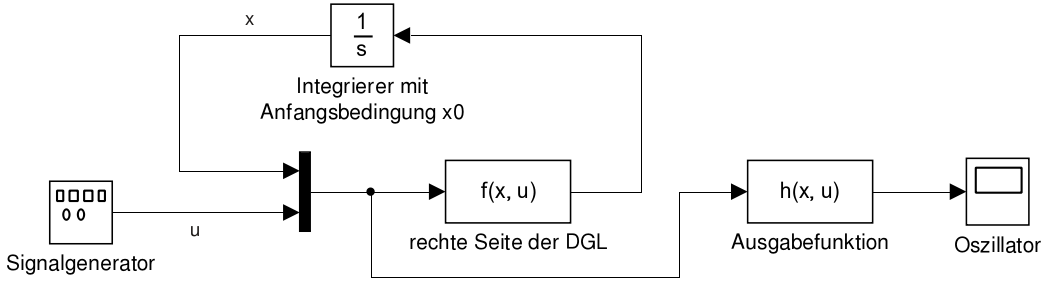
\includegraphics[scale=\modelscale]{dgl}
\end{center}
Den Ausgang erhält man dann einfach durch Anwendung von $h(\cdot, \cdot)$ auf
$x(\cdot)$ und $u(\cdot)$ (wie bei $\Sigma_1$).

\linie

\textbf{inverses Pendel}:
Ein \begriff{inverses Pendel (cart-pendulum system)} ist ein mathematisches Pendel,
das in der Ruhelage nach oben zeigt.
Das Pendel kann nur in einer Dimension schwingen und ist auf einem Wagen befestigt,
der sich in derselben Dimension hin- und her bewegen kann.
Der "`Wagen"' ist so gebaut, dass das Pendel auch nach unten schwingen kann,
es kann also die \SI{360}{\degree} voll ausnutzen.
Das Ziel ist, das Pendel durch Bewegung des Wagens in seiner instabilen Ruhelage zu halten.
Ein Segway kann vereinfacht als inverses Pendel betrachtet werden.

Bezeichnet man
die Masse am Pendel mit $m$,
die Masse des Wagens mit $M$,
die zurückgelegte Strecke des Wagens mit $p$,
die auf den Wagen wirkende Kraft mit $F$,
die Länge des Pendels mit $\ell$ und
den Winkel der Auslenkung des Pendels aus der Ruhelage mit $\theta$,
so erhält man mit den \begriff{\name{Lagrange}-Gleichungen}
$(M + m)\ddot{p} - m\ell \cos(\theta)\ddot{\theta} + c\dot{p} +
m\ell \sin(\theta)\dot{\theta}^2 = F$ sowie\\
$-m\ell \cos(\theta)\ddot{p} + m\ell^2\ddot{\theta} + \gamma \dot{\theta} -
mg\ell \sin(\theta) = 0$,
wobei $c$ und $\gamma$ den Reibungswiderstand des Wagens und des Pendels beschreiben.

Mit $U(\theta) := \smallpmatrix{M + m&-m\ell\cos(\theta)\\-m\ell\cos(\theta)&m\ell^2}$ und
$v(\theta, \dot{p}, \dot{\theta}) := \smallpmatrix{c\dot{p} + m\ell\sin(\theta)\dot{\theta}^2 \\
\gamma\dot{\theta} - mg\ell\sin(\theta)}$
kann man das System schreiben als $U(\theta) \smallpmatrix{\ddot{p} \\ \ddot{\theta}} +
v(\theta, \dot{p}, \dot{\theta}) = \smallpmatrix{F \\ 0}$.
Dabei ist $U(\theta)$ invertierbar, weil die Determinante für kein $\theta$ verschwindet.
Deswegen kann man dies schreiben als\\
$\smallpmatrix{\ddot{p} \\ \ddot{\theta}} = -U(\theta)^{-1} v(\theta, \dot{p}, \dot{\theta}) +
U(\theta)^{-1} \smallpmatrix{F \\ 0} =: \smallpmatrix{w_1(p, \theta, \dot{p}, \dot{\theta}, F) \\
w_2(p, \theta, \dot{p}, \dot{\theta}, F)}$.

Wenn man die Zustandsgrößen $\smallpmatrix{x_1 \\ x_2} := \smallpmatrix{p \\ \theta}$ und
$\smallpmatrix{x_3 \\ x_4} := \smallpmatrix{\dot{p} \\ \dot{\theta}}$
sowie die Eingangsgröße $u := F$ definiert,
so kann das System durch $\dot{x} = f(x, u)$ als System erster Ordnung beschrieben werden,
wobei $f(x, u) := \smallpmatrix{x_3 \\ x_4 \\ w_1(x, u) \\ w_2(x, u)}$.

\pagebreak

\subsection{%
    Gleichgewichte und Linearisierung%
}

\textbf{Gleichgewicht}:
Alle Paare von Vektoren $(x_e, u_e) \in X \times U$ mit $f(x_e, u_e) = 0$ heißen\\
\begriff{Gleichgewichte (equilibria)} des Systems $\dot{x} = f(x, u)$.

%Wenn ein System mit der konstanten Steuergröße $u(t) = u_e$ betrieben und
%der Zustand durch $x_e(t_0) = x_e$ initialisiert wird, so gilt für die Zustandsgröße
%$x(t) = x_e$ und $\dot{x}(t) = 0$ für alle $t \ge t_0$,
%d.\,h. wenn ein System im Gleichgewicht startet,
%dann bleibt die Zustandsgröße auch da.

Wenn ein System mit der konstanten Steuergröße $u(t) = u_e$ betrieben wird,
der Zustand durch $x_e(t_0) = x_e$ initialisiert wird und die Lösung des Systems eindeutig ist,
dann gilt $x(t) \equiv x_e$ für alle $t \ge t_0$
(weil das eine Lösung ist, da $f(x_e, u_e) = 0$).

\textbf{Beispiel}:
Für Gleichgewichte in obiger DGL müssen die Ableitungen von $p$ und $\theta$ verschwinden,
also $0 = F$ und $-mg\ell \sin(\theta) = 0$.
Die Lösungen sind $\theta_e = 0$ (aufrechte Position) und $\theta_e = \pi$ (nach unten zeigend),
wobei $p_e$ beliebig ist.

\linie

\textbf{Herleitung der Linearisierung}:
Falls $f$ und $h$ stetig dif"|ferenzierbar sind, kann man die Taylorentwicklungen erster Ordnung
um $(x_e, u_e)$ berechnen als\\
$f(x, u) \approx f(x_e, u_e) + \partial_x f(x_e, u_e) (x - x_e) +
\partial_u f(x_e, u_e) (u - u_e)$ und\\
$h(x, u) \approx y_e + \partial_x h(x_e, u_e) (x - x_e) +
\partial_u h(x_e, u_e) (u - u_e)$, wobei $y_e := h(x_e, u_e)$.\\
Dabei sind die partiellen Ableitungen die Jacobi-Matrizen.
Die Näherung ist besonders gut, falls $x \approx x_e$ und $u \approx u_e$.
Daher kann man die Entwicklungen zur Linearisierung von nicht-linearen Systemen verwenden.

\textbf{Linearisierung}:
Seien $f(x_e, u_e) = 0$ und $f, h \in \C^1$.
Dann ist die \begriff{Linearisierung (linearization)} von $\dot{x} = f(x, u)$, $y = h(x, u)$
bei $(x_e, u_e)$ gegeben durch
$\dot{x}_\Delta = A x_\Delta + B u_\Delta$, $y_\Delta = C x_\Delta, + D u_\Delta$,
wobei $A := \partial_x f(x_e, u_e)$, $B := \partial_u f(x_e, u_e)$,
$C := \partial_x h(x_e, u_e)$, $D := \partial_u h(x_e, u_e)$.

Für die betrachteten $t$ gelte $u(t) \approx u_e$ und $x(t) \approx x_e$.
Für die nicht-lineare Ausgangsgröße gilt also $y(t) \approx y_e$.
Wenn man nun die Linearisierung mit $u_\Delta := u(t) - u_e$ für den Anfangswert
$x_\Delta(0) := x(0) - x_e$ ausführt, so hofft man, dass
$y_e + y_\Delta(t)$ die nicht-lineare Ausgangsgröße $y(t)$ gut approximiert.\\
Es gilt nämlich $\left[x(t) - x_e\right]^\cdot = \dot{x}(t) = f(x(t), u(t)) \approx
A[x(t) - x_e] + Bu_\Delta(t)$ nach Definition der Linearisierung
($(x_e, u_e)$ ist nämlich ein Gleichgewicht).
Wenn die Trajektorie $x(\cdot)$ nahe an $x_e$ bleibt, dann ist die Taylor-Abschätzung
besonders gut -- würde ein Gleichheitszeichen stehen, dann wäre $[x(t) - x_e]$
ebenfalls eine Lösung der Linearisierung, es müsste also $x_\Delta(t) = x(t) - x_e$ gelten.
Aufgrund der nur ungefähren Gleichheit gilt aber nur $x_\Delta(t) \approx x(t) - x_e$.\\
Außerdem gilt $\left[y(t) - y_e\right] = h(x(t), u(t)) - y_e \approx C[x(t) - x_e] + Du_\Delta(t)$.
Für $x_\Delta(t) \approx x(t) - x_e$ ist die rechte Seite ungefähr gleich $y_\Delta(t)$,
also $y_\Delta(t) \approx y(t) - y_e$.
So erhält man $y(t) \approx y_e + y_\Delta(t)$.

\linie

\textbf{Beispiel}:
Man betrachtet das inverse Pendel im nach unten zeigenden, stabilen Gleichgewicht.
Wenn man nur kurz eine Kraft anwendet, dann schlägt das Pendel nur kurz in beide Richtungen
aus, ehe es sich wieder im Gleichgewicht befindet.
Weil keine großen Abweichungen der Position auftreten, ist die zugehörige Linearisierung eine
ziemlich gute Annäherung.\\
Anders sieht es aus, wenn man das Pendel im oberen, instabilen Gleichgewicht startet
und dieselbe Kraft kurz anwendet.
Dann wird das Pendel nach unten schwingen und sich im unteren Gleichgewicht einpendeln.
Wegen der großen Abweichungen der Position zur Startposition ist die Linearisierung für
das obere Gleichgewicht keine gute Annäherung.

\pagebreak

\subsection{%
    Systemverbindungen und Blockdiagramme%
}

\begriff{Modularität} ist eines der wichtigsten Konzepte bei der Modellierung von
dynamischen Systemen.
Komplexe Modelle werden durch Verbindung einfacher Systemkomponenten in einer Art Hierarchie
verbunden.
Die \begriff{Verbindung} geschieht dabei durch Gleichsetzung von Signalen.

\textbf{Vorteile der Modularität}:
\begin{itemize}
    \item
    Benutzung von Softwarebibliotheken mit Standard-Systemkomponenten und
    Schnittstellen zwischen verschiedenen physikalischen Bereichen

    \item
    Benutzung von Modellierungspaketen (MATLAB, Modelica)

    \item
    Übersichtlichkeit auch bei komplexen Modellen durch die hierarchische, verschachtelte
    Struktur

    \item
    Veränderung von einzelnen Komponenten, ohne das Gesamtgefüge zu zerstören
\end{itemize}

\linie

\textbf{Beispiel}:
Beim inversen Pendel geht man davon aus, dass die Kraft des Wagens durch einen
elektrischen Gleichstrom-Motor an einem Rad mit Radius $r$ erzeugt wird.
Wenn die Spannung $V$ an den Motor angelegt wird, dann erzeugt der Strom in den Spulen
ein Drehmoment.
Wenn $T$ das Lastmoment des Motors ist, dann wird die Dynamik des Motors durch
$J\ddot{\phi} + b\dot{\phi} = k_m I - T$, $L\dot{I} + RI = V - k_e\dot{\phi}$
beschrieben, wobei $J, b, k_m, L, R, k_e > 0$ konstant sind.
Man nimmt an, dass das Lastmoment und der Winkel der Motorwelle durch
$T = Fr$ und $p = r\phi$ mit $F$ und $p$ zusammenhängen.
Diese Gleichungen muss man nun mit der ursprünglichen DGL des inversen Pendels kombinieren.
Man erhält dann
$L\dot{I} + RI + \frac{k_e}{r}\dot{p} = V$,\\
$\left(M + m + \frac{J}{r^2}\right)\ddot{p} - m\ell \cos(\theta)\ddot{\theta} +
\left(c + \frac{b}{r^2}\right)\dot{p} + m\ell \sin(\theta)\dot{\theta}^2 -
\frac{k_m}{r}I = 0$ sowie\\
$-m\ell \cos(\theta)\ddot{p} + m\ell^2\ddot{\theta} + \gamma \dot{\theta} -
mg\ell \sin(\theta) = 0$.\\
Die gekoppelten Gleichungen heißen oft auch \begriff{beidseitig gekoppelt},
weil sich die Dynamik beider Systeme gegenseitig beeinflusst.
Für $k_e = 0$ wäre die Kopplung \begriff{einseitig}
(die erste Gleichung könnte dann separat gelöst werden).\\
In der Simulation erkennt man, dass für kleines $L$ (Motor kann die Kraft schnell aufwenden)
die Lösung sich kaum von der Lösung ohne Motor unterscheidet.
Für größeres $L$ (nur langsame Aufwendung der Kraft) unterscheiden sich
die beiden Systeme jedoch erheblich.

\linie

\textbf{Reihenschaltung}:
Die \begriff{Reihenschaltung (series interconnection)} der Systeme\\
$\dot{x}_1 = f_1(x_1, u_1)$, $y_1 = h_1(x_1, u_1)$ und
$\dot{x}_2 = f_2(x_2, u_2)$, $y_2 = h_2(x_2, u_2)$
erhält man, wenn man den Ausgang des ersten Systems mit dem Eingang des zweiten Systems
verbindet, also $u_2 = y_1$
(dabei müssen die Dimensionen übereinstimmen).
Man erhält das System\\
$\dot{x} = f(x, u_1)$, $y_2 = h_2(x_2, h_1(x_1, u_1))$,
wobei $x := \smallpmatrix{x_1 \\ x_2}$ und
$f(x, u_1) := \smallpmatrix{f_1(x_1, u_1) \\ f_2(x_2, h_1(x_1, u_1))}$.

Für lineare Systeme
$\dot{x}_1 = A_1 x_1 + B_1 u_1$, $y_1 = C_1 x_1 + D_1 u_1$ und\\
$\dot{x}_2 = A_2 x_2 + B_2 u_2$, $y_2 = C_2 x_2 + D_2 u_2$ entspricht dies
$\dot{x} = Ax + Bu_1$, $y_2 = Cx + Du_1$\\
mit $x := \smallpmatrix{x_1 \\ x_2}$ sowie
$A := \smallpmatrix{A_1 & 0 \\ B_2 C_1 & A_2}$,
$B := \smallpmatrix{B_1 \\ B_2 D_1}$,
$C := \smallpmatrix{D_2 C_1 & C_2}$ und
$D := D_2 D_1$.

\linie

\textbf{Parallelschaltung}:
Die \begriff{Parallelschaltung (parallel interconnection)} der Systeme\\
$\dot{x}_1 = f_1(x_1, u_1)$, $y_1 = h_1(x_1, u_1)$ und
$\dot{x}_2 = f_2(x_2, u_2)$, $y_2 = h_2(x_2, u_2)$
erhält man, wenn beide denselben Eingang haben und man die Ausgänge summiert,
also $u_1 = u_2 = u$ und $y = y_1 + y_2$
(dabei müssen die Dimensionen übereinstimmen).
Man erhält das System\\
$\dot{x} = f(x, u)$, $y = h_1(x_1, u) + h_2(x_2, u)$,
wobei $x := \smallpmatrix{x_1 \\ x_2}$ und
$f(x, u) := \smallpmatrix{f_1(x_1, u) \\ f_2(x_2, u)}$.

Für lineare Systeme
$\dot{x}_1 = A_1 x_1 + B_1 u_1$, $y_1 = C_1 x_1 + D_1 u_1$ und\\
$\dot{x}_2 = A_2 x_2 + B_2 u_2$, $y_2 = C_2 x_2 + D_2 u_2$ entspricht dies
$\dot{x} = Ax + Bu$, $y = Cx + Du$\\
mit $x := \smallpmatrix{x_1 \\ x_2}$ sowie
$A := \smallpmatrix{A_1 & 0 \\ 0 & A_2}$,
$B := \smallpmatrix{B_1 \\ B_2}$,
$C := \smallpmatrix{C_1 & C_2}$ und
$D := D_1 + D_2$.

\linie
\pagebreak

\textbf{Control System Toolbox}:
Die \begriff{Control System Toolbox} von MATLAB stellt sog. \begriff{\code{ss}-Objekte} bereit,
die lineare Systeme darstellen.
Die Verwendung erfolgt wie folgt:
\begin{itemize}
    \item
    Definition: \code{sys = ss(A, B, C, D)}

    \item
    Reihenschaltung: \code{sys = sys1 * sys2}

    \item
    Parallelschaltung: \code{sys = sys1 + sys2}

    \item
    Simulation: \code{y = lsim(sys, u, T, x0)}

    \item
    Bestimmung der definierenden Matrizen: \code{[A, B, C, D] = ssdata(sys)}
\end{itemize}
Die überladenen Operatoren \code{*} und \code{+} erinnern an die zugehörigen Operationen
der Matrizen, die bei der Bildung der Reihen- bzw. Parallelschaltung verwendet werden.

\linie

\textbf{Blockdiagramm}:
Ein \begriff{Blockdiagramm (block-diagram)} besteht aus Verbindungen von einzelnen Blöcken.
Solche Diagramme sollten bestimmten algebraischen Gleichungen entsprechen.

\textbf{Beispiele}:
\begin{itemize}
    \item
    \textbf{Reihenschaltung}:\\
    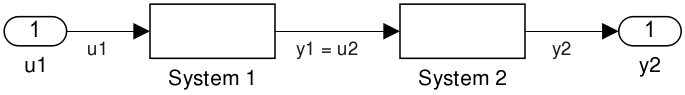
\includegraphics[scale=\modelscale]{schaltung_reihe.png}

    \item
    \textbf{Parallelschaltung}:\\
    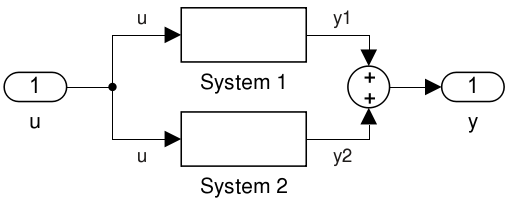
\includegraphics[scale=\modelscale]{schaltung_parallel.png}

    \item
    \textbf{gedämpftes Federpendel}:\\
    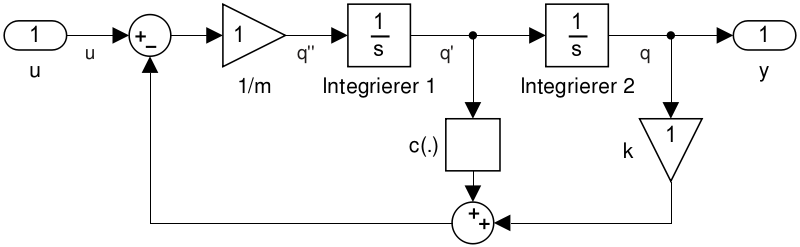
\includegraphics[scale=\modelscale]{federpendel_gedaempft.png}

    \item
    \textbf{allgemeines lineares System}:
    (in Simulink auch darstellbar durch einen \code{State-Space}- oder \code{LTI Systems}-Block,
    definiert durch $A, B, C, D$ bzw. ein \code{ss}-Objekt)\\
    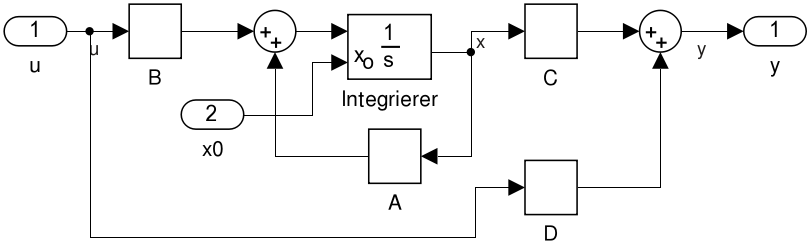
\includegraphics[scale=\modelscale]{lineares_system.png}
\end{itemize}

\pagebreak

\section{%
    Symmetrische Verschlüsselungsverfahren%
}

\subsection{%
    Definitionen%
}

\textbf{kryptografisches Verschlüsselungsverfahren}:
Ein \begriff{(kryptografisches) Verschlüsselungsver"-fahren}
(auch \begriff{kryptografisches System} oder \begriff{Kryptosystem})
$(P, C, K, (c_k)_{k \in K}, (d_k)_{k \in K})$ wird definiert durch endliche Mengen
\begin{itemize}
    \item
    $P$ (\begriff{Klartexte}),

    \item
    $C$ (\begriff{Geheimtexte}) und

    \item
    $K$ (\begriff{Schlüssel})
\end{itemize}
sowie durch Funktionen für jeden Schlüssel $k \in K$ mit
\begin{itemize}
    \item
    $c_k\colon P \rightarrow C$ (\begriff{Codierungs-/Verschlüsselungsfunktion}) und

    \item
    $d_k\colon C \rightarrow P$ (\begriff{Decodierungs-/Entschlüsselungsfunktion}),
\end{itemize}
sodass $\forall_{k \in K} \exists_{\ell \in K} \forall_{x \in P}\; d_\ell(c_k(x)) = x$
(\begriff{Korrektheit des Verfahrens}).

Aus der Korrektheit folgt für alle $k \in K$, dass $c_k$ injektiv ist
(für $x_1, x_2 \in P$ mit $c_k(x_1) = c_k(x_2)$ gilt
$x_1 = d_\ell(c_k(x_1)) = d_\ell(c_k(x_2)) = x_2$).

\textbf{symmetrisches Verfahren}:
Das Verfahren heißt \begriff{symmetrisch} (oder \begriff{Private-Key-Verfahren}), falls
in obiger Definition $\ell = k$ oder $\ell$ sich leicht aus $k$ berechnen lässt.

In diesem Kapitel werden nur symmetrische Verfahren betrachtet.

\linie

\textbf{kryptografisches Szenario}:
Das typische Szenario bei symmetrischen Verfahren ist wie folgt.
Alice will Bob eine Nachricht schicken und Eve (\emph{eavesdropper}) will mithören.
\begin{enumerate}
    \item
    Alice und Bob wählen einen gemeinsamen Schlüssel $k \in K$.
    Dieser ist beiden vor der Übertragung schon bekannt oder wird über einen
    sicheren Kanal übermittelt.

    \item
    Alice verschlüsselt $x \in P$ durch $y = c_k(x)$ und sendet $y$ an Bob.

    \item
    Bob empfängt $y$ und entschlüsselt $y$ durch $d_k(y) = d_k(c_k(x)) = x$.
\end{enumerate}
Eve, die mithören will, kann nur $y$ abfangen (nicht den Schlüssel $k$).
Mit dieser Information startet sie ihre \begriff{Kryptanalyse}.

\pagebreak

\subsection{%
    Kryptanalyse%
}

\textbf{\name{Kerckhoffs}' Prinzip}:
Die Sicherheit eines Verfahrens darf nur auf der Geheimhaltung des Schlüssels basieren,
nicht aber auf der Geheimhaltung des Verfahrens.
Angreifer kennen also zumindest das verwendete kryptografische System.

\linie

\textbf{Kompromittierung von kryptografischer Kommunikation}:
\begin{itemize}
    \item
    \begriff{Bruch des Schlüssels}:
    Eve kann nicht nur Nachrichten entschlüsseln und lesen, sondern auch
    Fehlnachrichten verschlüsseln und verschicken

    \item
    \begriff{globale Lösung}:
    funktionierendes Entschlüsselungsverfahren ohne Kenntnis des Schlüssels\\
    (Eve kann keine Fehlnachrichten verschlüsseln)

    \item
    \begriff{lokale Lösung}:
    nur eine einzelne Nachricht entschlüsselt

    \item
    \begriff{Informationsgewinn}:
    partielle Informationen über Schlüssel oder Klartext
\end{itemize}

\linie

\textbf{Angriffsszenarien}:
\begin{itemize}
    \item
    \begriff{ausschließlich Geheimtext (ciphertext-only)}:
    Eve kennt nur Geheimtexte

    \item
    \begriff{bekannter Klartext (known-plaintext)}:
    Eve kennt Klartexte und zugehörige Geheimtexte

    \item
    \begriff{gewählter Klartext (chosen-plaintext)}:
    Eve kann Klartexte verschlüsseln lassen

    \item
    \begriff{gewählter Geheimtext (chosen-ciphertext)}:
    Eve kann Geheimtexte entschlüsseln lassen
\end{itemize}

\linie

\textbf{Sicherheitsstufen eines Verfahrens}:
\begin{itemize}
    \item
    \begriff{perfekte/absolute Sicherheit}:
    Entschlüsselung beweisbar unmöglich

    \item
    \begriff{Berechnungssicherheit}:
    Entschlüsselung beweisbar für die Praxis zu aufwändig

    \item
    \begriff{relative Berechnungssicherheit}:
    Entschlüsselung mindestens so schwer wie die Lösung eines als schwierig geltenden Problems

    \item
    \begriff{pragmatische Sicherheit}:
    trotz intensiver Suche keine ef"|fiziente Methode zur Entschlüsselung bekannt
\end{itemize}
In der Praxis tritt bei der klassischen Kryptografie die pragmatische Sicherheit am häufigsten auf.
Allerdings können Verfahren schwieriger zu brechen scheinen, als sie es sind, und
außerdem könnten geheime Hintertüren in Verfahren eingebaut sein.

\pagebreak

\subsection{%
    Blockchif"|fren%
}

\textbf{Blockchif"|fre}:
Seien $n \in \natural$ und $\Sigma$ ein Alphabet (eine endliche Menge).
Eine \begriff{Blockchif"|fre} mit \begriff{Blocklänge} $n$
ist ein symmetrisches Verschlüsselungsverfahren mit $P = C := \Sigma^n$.

Bei einer Blockchif"|fre wird zur Verschlüsselung eines beliebigen Texts $w \in \Sigma^\ast$ der
Text in Blöcke der Länge $n$ aufgeteilt.
Anschließend wird jeder Block mit demselben Schlüssel verschlüsselt.

\linie

\textbf{Lemma (Blockchif"|fren sind Permutationen)}:
Codierungsfunktionen einer Blockchif"|fre sind Permutationen von $\Sigma^n$
und die Decodierungsfunktionen sind die inversen Permutationen.

\begin{Beweis}
    Für alle $k \in K$ ist $c_k\colon \Sigma^n \rightarrow \Sigma^n$
    injektiv und damit bijektiv (\emph{pigeonhole principle}).
    Weil das Verfahren symmetrisch ist, gilt die Korrektheit in der Form
    $\forall_{k \in K} \forall_{x \in P}\; d_k(c_k(x)) = x$, für
    alle $k \in K$ ist also $d_k = c_k^{-1}$ bijektiv.
\end{Beweis}

Es wäre unpraktikabel, als Codierungsfunktion $c_k$ einer Blockchif"|fre jede Permutation
zuzulassen (d.\,h. $K$ gleich der Menge der Permutationen von $\Sigma^n$ und
$c_\sigma := \sigma$ für $\sigma \in K$),
denn um einen Schlüssel zu speichern, benötigt man Platz $\Omega(|\Sigma|^n)$.
Daher schränkt man die Anzahl der möglichen Permutationen ein,
wofür es im Wesentlichen drei Möglichkeiten gibt
(mono- und polyalphabetische Substitution sowie Permutationschif"|fre).

\subsection{%
    Monoalphabetische Substitution%
}

\textbf{monoalphabetische Verschiebung}:
Sei $P = C = K := \integer/26\integer$ (Alphabet $\Sigma := \{\code{a}, \dotsc, \code{z}\}$
wird mit $\integer/26\integer$ identifiziert).
Dann ist die \begriff{monoalphabetische Verschiebung} eine Blockchif"|fre mit Blocklänge $1$,
die definiert ist durch $c_k(x) := x + k$ und $d_k(x) := x - k$ für $k \in K$.

\textbf{\name{Caesar}-Verfahren}:
monoalphabetische Verschiebung mit Schlüssel $k = 3$

\textbf{ROT13}:
monoalphabetische Verschiebung mit Schlüssel $k = 13$ (Spezialfall, da $c_k = d_k$)

\textbf{Angriff}:
\begriff{Brute-Force} (alle Möglichkeiten durchprobieren),
da der Schlüsselraum nur aus $|\Sigma|$ vielen Schlüsseln besteht.

\linie

\textbf{monoalphabetische Substitution}:
Seien $P = C := \Sigma$ und
$K := \{\sigma \;|\; \sigma \text{ Permutation von } \Sigma\}$.\\
Dann ist die \begriff{monoalphabetische Substitution} eine Blockchif"|fre mit Blocklänge $1$,
die definiert ist durch
$c_\sigma := \sigma$ und $d_\sigma := \sigma^{-1}$ für $\sigma \in K$.

Die monoalphabetische Verschiebung ist eine monoalphabetische Substitution
($\Sigma := \integer/26\integer$ und für $\sigma = k \in \integer/26\integer$ ist
$c_\sigma = \smallpmatrix{0 & 1 & \cdots & 25 \\ k & k + 1 & \cdots & k - 1}$).

\textbf{Angriff (Häufigkeitsanalyse)}:
Die Größe des Schlüsselraums ist $|K| = |\Sigma|!$, für $n = 26$ gilt also
$|K| = 26! \approx 10^{26}$.
Brute-Force ist bei solchen Größenordnungen nicht praktikabel.
Stattdessen führt man eine \begriff{Häufigkeitsanalyse} durch.
Dazu nutzt man aus, dass bei Klartexten in natürlichen Sprachen bestimmte
Zeichen aus $\Sigma$ häufiger vorkommen als andere.
%In der deutschen Sprache kommt z.\,B. das \code{e} am häufigsten vor.
Da die monoalphabetische Substitution diese Häufigkeiten invariant lässt, kann man dem
häufigsten Geheimtext-Zeichen das \code{e} zuordnen und evtl. dem zweithäufigsten das \code{n}.
Dies lässt sich auch für häufig auftretende Doppellaute durchführen (\code{en}, \code{er}, \dots).
Weitere Zuordnungen können aus dem Kontext erschlossen werden
(es gibt nur bestimmte Kombinationen von Klartext-Zeichen zu sinnvollen Wörtern).
Eine Abhilfe gegen diese überflüssigen Kontextinformationen kann Datenkompression sein
(um den Angriff zu erschweren).

\pagebreak

\subsection{%
    Polyalphabetische Substitution%
}

\textbf{polyalphabetische Substitution}:
Eine \begriff{polyalphabetische Substitution} ist ein Blockchif"|fre mit Blocklänge $n$,
bei dem jeder Klartext-Buchstabe einzeln permutiert wird, d.\,h.\\
$P = C := \Sigma^n$ und $K := \{\sigma \;|\; \sigma \text{ Permutation von } \Sigma\}^n$ sowie\\
$c_\sigma(x) := \sigma_1(x_1) \dotsb \sigma_n(x_n)$ und
$d_\sigma(x) := \sigma^{-1}_1(x_1) \dotsb \sigma^{-1}_n(x_n)$ für $\sigma \in K$.

\textbf{\name{Vigenère}-Verfahren}:
Seien $P = C := \Sigma^n$ und $K := \Sigma^d$ für ein festes $d \in \natural$.\\
Dann ist das \begriff{\name{Vigenère}-Verfahren mit Schlüssellänge $d$} eine
Blockchif"|fre mit Blocklänge $n$, die definiert ist durch
$c_k(x) := \widetilde{c}(x_1, k_{0 \bmod d}) \widetilde{c}(x_2, k_{1 \bmod d}) \cdots
\widetilde{c}(x_n, k_{(n-1) \bmod d})$ für $x =: x_1 \cdots x_n$ und
$k =: k_0 \dotsb k_{d-1} \in K$, wobei
$\widetilde{c}(a, k_i) := a + k_i$ für $a \in \Sigma$ und $i = 0, \dotsc, d - 1$\\
(es wird angenommen, dass $\Sigma$ geordnet ist, d.\,h.
$\widetilde{c}(\cdot, k_i)$ ist die Verschiebung um $k_i$).

Vigenère-Verfahren sind polyalph. Subst.en
(die Permutationen sind einfache Verschiebungen).
Monoalph. Verschiebungen sind Vigenère-Verfahren mit Schlüssellänge $1$,
allerdings sind monoalph. Subst.en i.\,A. keine Vigenère-Verfahren.
Polyalph. Subst.en über $\Sigma$ können als monoalph. Subst.en über
$\Sigma' := \Sigma^n$ angesehen werden.

Vorteile des Vigenère-Verfahrens gegenüber der monoalphabetischen Substitution sind
eine gleichmäßigere Verteilung der Geheimtext-Zeichen und Elimination von Doppellauten.

\textbf{Angriff}:
Gleiche Klartextstellen werden gleich verschlüsselt, wenn der Abstand zwischen ihnen ein Vielfaches
der Schlüssellänge $d$ ist.
Kennt man daher die Schlüssellänge $d$ (oder auch nur ein Vielfaches von ihr),
dann kann man den Geheimtext $y$ in $d$ Spalten schreiben
(die $i$-te Spalte enthält die Zeichen $y_j$ mit $j \equiv i \mod d$).
Jede einzelne Spalte wurde durch eine eine monoalphabetische Verschiebung verschlüsselt und kann
dementsprechend mit Brute-Force oder Häufigkeitsanalyse leicht geknackt werden.

\linie

Um die Schlüssellänge $d$ oder ein Vielfaches dieser herauszufinden, muss man etwas arbeiten.

\textbf{Koinzidenz-Index}:
Seien $\Sigma$ ein Alphabet, $n \in \natural$ und $x, x' \in \Sigma^n$.\\
Dann heißt $\kappa(x, x') := \frac{1}{n} \sum_{i=1}^n \delta_{x_i,x_i'}$
\begriff{Koinzidenz-Index} von $x$ und $x'$.

Sind $x$ und $x'$ aus einem gleichverteilten Zufallsexperiment entstanden, dann gilt
$\EE[\kappa] = \frac{1}{|\Sigma|}$.
Für $|\Sigma| = 26$ gilt $\EE[\kappa] = \SI{3.8}{\percent}$.
Allerdings erhält man experimentell $\EE[\kappa] \approx \SI{7}{\percent}$ für
natürlich erzeugte Texte.
Wenn man sich zunutze macht, dass der Koinzidenz-Index zweier Klartexte bei
polyalphabetischer Substitution mit demselben Schlüssel
nicht ändert, d.\,h. $\kappa(x, x') = \kappa(c_k(x), c_k(x'))$,
dann lässt sich die Schlüssellänge einfach bestimmen.

Seien $y \in \Sigma^n$ ein Geheimtext und $\kappa^k := \kappa(y, \sigma^k(y))$ für
$k \in \natural$, wobei $\sigma^k(y)$ die zyklische Verschiebung von $y$ um $k$ Zeichen nach links
ist.
Für $k \in \natural$ mit $d \teilt k$ werden $x$ und $\sigma^k(x)$ mit demselben Schlüssel
Vigenère-verschlüsselt (bis auf das Ende), d.\,h. $\kappa^k$ wird für diese $k$ bei
ca. \SI{7}{\percent} liegen und für andere bei deutlich weniger.

Der Angriff durch das Koinzidenz-Kriterium ist für allgemeine polyalphabetische Substitutionen
durchführbar und damit sind diese Verfahren leicht angreifbar.
Trotzdem sind sie heute noch relevant
(z.\,B. kommerzielle Software, US-Mobiltelefone, oberflächlicher Schutz).

\pagebreak

\subsection{%
    Perfekte Sicherheit%
}

\textbf{Wahrscheinlichkeiten}:
Mit $\Pr(x)$ und $\Pr(y)$ werden die \begriff{Wahrscheinlichkeiten} bezeichnet,
dass Eve den Klartext $x$ bzw. den Geheimtext $y = c_k(x)$ für ein $k \in K$ abfängt.
Die Wahrscheinlichkeit, dass der Schlüssel $k \in K$ verwendet wird, wird mit $\Pr(k)$
bezeichnet.\\
$\Pr(y \;|\; x)$ und $\Pr(x \;|\; y)$ bezeichnen die Wahrscheinlichkeiten, dass $y$ abgefangen
wird unter der Bedingung, dass der zugehörige Klartext $x$ ist, bzw. umgekehrt.

$\Pr(y)$ wird durch $\Pr(x)$ und $\Pr(k)$ induziert.
In der Praxis gilt meist, dass $x$ und $k$ unabhängig sind (d.\,h. $\Pr(x, k) = \Pr(x) \Pr(k)$
für alle $x \in P$ und $k \in K$).
OBdA kann man annehmen, dass $\Pr(x) > 0$ und $\Pr(y) > 0$ für alle
$x \in P$ und $y \in C$ (sonst schränkt man $P$ und $C$ ein).

\textbf{perfekte Sicherheit}:
Ein Verschlüsselungsverfahren hat \begriff{perfekte Sicherheit}, falls\\
$\Pr(x \;|\; y) = \Pr(x)$ für alle $x \in P$ und $y \in C$.

Das heißt, dass die Kenntnis von $y$ keine Information über den Klartext $x$ bringt.

\linie

\textbf{Satz (notwendige Bedingung für perfekte Sicherheit)}:\\
Ist ein Verschlüsselungsverfahren perfekt sicher, so gilt
$|P| \le |C| \le |K|$.

\begin{Beweis}
    Für alle $k \in K$ ist $c_k\colon P \rightarrow C$ injektiv, d.\,h. $|P| \le |C|$.

    Sei $x \in P$ fest.
    Dann gibt es für jedes $y \in C$ ein $k_y \in K$ mit $c_{k_y}(x) = y$.
    Sonst gäbe es ein $y \in C$ mit $c_k(x) \not= y$ für alle $k \in K$,
    also $\Pr(x \;|\; y) = 0 < \Pr(x)$, ein Widerspruch zur perfekten Sicherheit.
    Aus $k_{y_1} = k_{y_2}$ folgt $y_1 = c_{k_{y_1}}(x) = c_{k_{y_2}}(x) = y_2$,
    d.\,h. $|C| \le |K|$.
\end{Beweis}

\linie

\textbf{Satz (Charakterisierung von perfekt sicheren Verfahren)}:
Seien  $|P| = |C| = |K|$ und Schlüssel- und Klartext-Wahrscheinlichkeiten voneinander unabhängig.
Dann ist das Verfahren perfekt sicher genau dann, wenn
$\forall_{k \in K}\; \Pr(k) = \frac{1}{|K|}$ und
$\forall_{x \in P} \forall_{y \in C} \exists!_{k_{x,y} \in K}\; c_{k_{xy}}(x) = y$ gilt.

\begin{Beweis}
    "`$\Rightarrow$"':
    Sei das Verfahren perfekt sicher.
    Wie im Beweis des vorherigen Satzes gibt es für alle $x \in P$ und $y \in C$ ein
    $k_{x,y} \in K$ mit $c_{k_{x,y}}(x) = y$,
    wobei $k_{x,y_1} \not= k_{x,y_2}$ für $y_1 \not= y_2$.
    Die Abbildung $f_x\colon C \rightarrow K$, $y \mapsto k_{x,y}$ ist für alle $x \in P$
    injektiv und wegen $|C| = |K|$ daher bijektiv, weswegen $k_{x,y} \in K$ eindeutig bestimmt ist.

    Sei nun $y \in C$ fest.
    Mit dem Satz von Bayes gilt $\Pr(x) = \Pr(x \;|\; y) = \frac{\Pr(y \;|\; x) \Pr(x)}{\Pr(y)}$,
    also $\Pr(y \;|\; x) = \Pr(y)$.
    Allerdings ist $\Pr(y \;|\; x) = \Pr(k_{xy})$, d.\,h.
    $\Pr(k_{xy}) = \Pr(y)$ für alle $x \in P$.
    Wie eben ist $g_y\colon P \rightarrow K$, $x \mapsto k_{x,y}$ bijektiv, d.\,h.
    $\Pr(k) = \Pr(y)$ ist für alle $k \in K$ gleich.

    "`$\Leftarrow$"':
    Es gilt $\Pr(y) = \sum_{x \in P} \Pr(y \;|\; x) \Pr(x)$
    (Gesetz der totalen Wahrscheinlichkeit).
    Weil die Schlüssel $k_{xy}$ eindeutig sind, gilt
    $\Pr(y \;|\; x) = \Pr(k_{xy}) = \frac{1}{|K|}$, also
    $\Pr(y) = \sum_{x \in P} \frac{1}{|K|} \Pr(x) = \frac{1}{|K|}$ wegen $|P| = |K|$.
    Damit gilt $\Pr(x \;|\; y) = \frac{\Pr(y \;|\; x) \Pr(x)}{\Pr(y)} = \Pr(x)$
    (perfekte Sicherheit).
\end{Beweis}

\pagebreak

\subsection{%
    One-Time-Pad%
}

\textbf{One-Time-Pad}:
Seien $P = C = K := \{0, 1\}^n$.
Dann ist das \begriff{(\name{Vernam}-)One-Time-Pad} eine Blockchif"|fre mit Blocklänge $n$,
die definiert ist durch $c_k(x) = x \xor k$ und $d_k(y) = y \xor k$ für $k \in \{0, 1\}^n$.

Dabei ist "`$\xor$"' das bitweise XOR
(Addition der Argumente, wenn man sie als Elemente von $(\integer/2\integer)^n$ auf"|fasst).
One-Time-Pads sind also genau die Vigenère-Verfahren über dem Alphabet $\{0, 1\}$
mit Schlüssellänge $n$.

One-Time-Pads sind perfekt sichere Verfahren im obigen Sinne.
Jeder Klartext ist möglich, wenn man den Schlüssel nicht kennt.
Wenn Eve z.\,B. die Nachricht \code{xsvii} abfängt, kann der Klartext \code{sonne} lauten
(mit dem Schlüssel \code{feive}) oder aber \code{regen} (mit dem Schlüssel \code{gopev}).
Dies gilt aber nur, wenn derselbe Schlüssel nur einmal verwendet wird:
Sind $y_1 = c_k(x_1)$ und $y_2 = c_k(x_2)$ zwei verschiedene abgefangene Nachrichten,
die mit demselben Schlüssel verschlüsselt wurden, so gilt
$y_1 \xor y_2 = (x_1 \xor k) \xor (x_2 \xor k) = x_1 \xor x_2$.
Wenn $x_1$ und $x_2$ natürliche Texte sind, kommen verschiedene Zeichen in
$x_1 \xor x_2$ stark unterschiedlich häufig vor und man kann eine Häufigkeitsanalyse starten.
Außerdem sind One-Time-Pads anfällig gegenüber Known-Plaintext-Attacken:
Die Kenntnis eines einzigen Klartext-Geheimtext-Paars $(x, c_k(x))$ reicht aus, um mit
$x \xor c_k(x) = x \xor (x \xor k) = k$ den Schlüssel herauszufinden.

One-Time-Pads sind aus verschiedenen Gründen unpraktikabel
(langer Schlüssel, zufällige Erzeugung nicht-trivial).

\subsection{%
    Data Encryption Standard (DES)%
}

DES ist eine symmetrische binäre Blockchif"|fre
(Blocklänge von 64 Bit und eff. Schlüssellänge von 56 Bit), wurde 1977 eingeführt und 2001 durch
AES abgelöst, weil es als nicht mehr sicher genug galt.
Allerdings wird DES immer noch verwendet, Triple-DES gilt nach wie vor als sicher.
Im Wesentlichen sind zwar nur Brute-Force-Angrif"|fe bekannt,
diese enden aber heutzutage innerhalb eines Tages erfolgreich.

DES sollte gewisse Designziele erfüllen,
wie hohe Sicherheit,
vollständige Spezifikation,
gute Verständlichkeit,
Einhaltung von Kerkhoffs' Prinzip,
Verfügbarkeit für alle Benutzer,
Vielseitigkeit,
Ef"|fizienz und
Eignung für Hardware-Implementationen.

\textbf{Data Encryption Standard (DES)}:
Sei $\BB := \{0, 1\}$.\\
Der \begriff{Data Encryption Standard (DES)} ist eine Blockchif"|fre mit Blocklänge 64,
wobei $y := c_k(x)$ für $x \in \BB^{64}$ und $k \in \BB^{64}$ wie folgt definiert ist:
\begin{enumerate}
    \item
    Wende eine Initialpermutation $\IP\colon \BB^{64} \rightarrow \BB^{64}$ auf $x$ an
    (siehe unten) und teile das Ergebnis auf, d.\,h.
    $L_0 R_0 := \IP(x)$ mit $L_0, R_0 \in \BB^{32}$.

    \item
    Berechne sukzessive für $i = 1, \dotsc, 16$ die Wörter $L_i, R_i \in \BB^{32}$ durch\\
    $L_i := R_{i-1}$ und $R_i := L_{i-1} \xor f(R_{i-1}, k_i)$,
    wobei die Rundenfunktion $f\colon \BB^{32} \times \BB^{48} \rightarrow \BB^{32}$
    und der Rundenschlüssel $k_i \in \BB^{48}$ weiter unten definiert sind.

    \item
    Berechne $y := \IP^{-1}(R_{16} L_{16})$.
\end{enumerate}

\linie
\pagebreak

\textbf{Initialpermutation}:
Die \begriff{Initialpermutation} $\IP\colon \BB^{64} \rightarrow \BB^{64}$ ist statisch
definiert.\\
Ein Ausschnitt lautet $\IP(x_1 \cdots x_{64}) := x_{58} x_{50} x_{42} \cdots x_{15} x_7$.\\
Ein Ausschnitt der Inversen ist $\IP(x_1 \cdots x_{64}) := x_{40} x_8 x_{48} \cdots x_{57} x_{25}$.

\textbf{Rundenfunktion}:
Die \begriff{Rundenfunktion} (oder \begriff{interne Blockchif"|fre})
$f\colon \BB^{32} \times \BB^{48} \rightarrow \BB^{32}$,\\
$(A,J) \mapsto f(A,J)$
ist wie folgt definiert:
\begin{enumerate}
    \item
    Expandiere $A$ auf 48 Bit mittels der \begriff{Expandierungsfunktion}
    $E\colon \BB^{32} \rightarrow \BB^{48}$,
    wobei alle 32 Bit in $E(A)$ auftauchen und 16 der Bits an bestimmten Stellen wiederholt werden
    (ebenfalls statisch).

    \item
    Berechne $B := E(A) \xor J$ und zerlege das Ergebnis in $B =: B_1 \cdots B_8$ mit
    $B_i \in \BB^6$.

    \item
    Transformiere $B_i$ in $C_i := S_i(B_i) \in \BB^4$ mittels den sog. \begriff{S-Boxen}
    $S_i\colon \BB^6 \rightarrow \BB^4$
    (statisch).

    \item
    Bilde $C := C_1 \cdots C_8 \in \BB^{32}$ und wende eine statische Bitpermutation an:
    $f(A, J) := P(C)$.
\end{enumerate}
Die S-Boxen sind dabei als Tabellen der Größe $4 \times 16$ gegeben.
Für die Berechnung von\\
$C_i = S_i(B_i)$ sei $B_i =: b_{i,1} \cdots b_{i,6}$ mit
$b_{i,j} \in \BB$.
Dann wählt man die Zeile $(b_1 b_6)_2$ und die Spalte $(b_2 b_3 b_4 b_5)_2$ und die Zahl an dieser
Stelle in Binärdarstellung ist $C_i$
(die Nummerierung beginnt jeweils bei $0$).
Die S-Boxen (engl. \emph{substitution box}) sind nicht-lineare Komponenten, die verhindern,
dass die Verschlüsselung nur die Lösung eines LGS ist.

\textbf{Rundenschlüssel}:\\
Die \begriff{Rundenschlüssel} $k_1, \dotsc, k_{16} \in \BB^{48}$ werden aus
$k \in \BB^{64}$ wie folgt berechnet:
\begin{enumerate}
    \item
    Wähle bestimmte 56 Bit aus $k$ mittels der statischen Abbildung
    $\PC_1\colon \BB^{64} \rightarrow \BB^{56}$.

    \item
    Zerlege das Ergebnis in $C_0 D_0 := \PC_1(k)$ mit $C_0, D_0 \in \BB^{28}$.

    \item
    Berechne für $i = 1, \dotsc, 16$ die Wörter $C_i, D_i \in \BB^{28}$ durch
    $C_i := \sigma_i(C_{i-1})$ und\\
    $D_i := \sigma_i(D_{i-1})$, wobei $\sigma_i$ die zyklische Linksverschiebung um ein Bit
    für $i \in \{1, 2, 9, 16\}$ und um zwei Bit sonst ist.

    \item
    Wähle bestimmte 48 Bit aus $C_i D_i$ mittels der statischen Abbildung
    $\PC_2\colon \BB^{56} \rightarrow \BB^{48}$ und setze
    $k_i := \PC_2(C_i D_i)$.
\end{enumerate}

\linie

\textbf{DES-Entschlüsselung}:
Ein Geheimtext $y \in \BB^{64}$ wird entschlüsselt,
indem man den gleichen Algortihmus wie bei der Verschlüsselung anwendet,
nur muss man dieses Mal die Rundenschlüssel in umgekehrter Reihenfolge $k_{16}, \dotsc, k_1$
benutzen.

Diese einfache Art der Entschlüsselung ist günstig für die Hardware-Implementierung
(spart Schaltungsaufwand).

\textbf{Satz (Korrektheit der Entschlüsselung)}:
Für den so erhaltenen Text $z \in \BB^{64}$ gilt $z = x$.

\begin{Beweis}
    Bei der Entschlüsselung von $y \in \BB^{64}$ berechnet man zuerst
    $L_0' R_0' := \IP(y)$\\
    $= \IP(\IP^{-1}(R_{16} L_{16})) = R_{16} L_{16}$ mit
    $L_0', R_0' \in \BB^{32}$.
    Es gilt also $L_0' = R_{16}$ und $R_0' = L_{16}$.
    Induktiv beweist man nun $L_i' = R_{16-i}$ und $R_i' = L_{16-i}$ für $i = 0, \dotsc, 16$.
    Daraus folgt dann die Behauptung mit
    $z = \IP^{-1}(R_{16}' L_{16}') = \IP^{-1}(L_0 R_0) = \IP^{-1}(\IP(x)) = x$.

    Angenommen, es gilt $L_{i-1}' = R_{17-i}$ und $R_{i-1}' = L_{17-i}$ für ein
    $i \in \{1, \dotsc, 16\}$.\\
    Dann ist $L_i' := R_{i-1}' = L_{17-i} = R_{16-i}$ und
    $R_i' := L_{i-1}' \xor f(R_{i-1}', k_{17-i}) =
    R_{17-i} \xor f(L_{17-i}, k_{17-i})$\\
    $= (L_{16-i} \xor f(R_{16-i}, k_{17-i})) \xor f(L_{17-i}, k_{17-i})
    = (L_{16-i} \xor f(L_{17-i}, k_{17-i})) \xor f(L_{17-i}, k_{17-i}) = L_{16-i}$,
    weil die Rundenschlüssel in umgekehrter Reihenfolge benutzt werden.
\end{Beweis}

\pagebreak

\subsection{%
    Mehrfachverschlüsselung%
}

DES gilt wegen der kurzen ef"|fektiven Schlüssellänge von 56 Bit als unsicher.
Man kann das Problem beheben, in dem man DES mehrfach anwendet.

\textbf{Triple-DES}:
\begriff{Triple-DES} ist eine Blockchif"|fre mit Blocklänge 64, wobei man
$y := c_k(x)$ für $k := k_1 k_2 \in \BB^{128}$ mit $k_1, k_2 \in \BB^{64}$ wie folgt berechnet:
$y = \DES_{k_1}(\DES^{-1}_{k_2}(\DES_{k_1}(x)))$
(dabei bezeichnet $\DES_{k_i}$ die Anwendung von DES mit dem Schlüssel $k_i$).

Ef"|fektiv verwendet also nun eine Schlüssellänge von 112 Bit, was heutzutage als sicher gilt.
DES ist nicht unter Komposition abgeschlossen, d.\,h.
$\exists_{k_1, k_2 \in \BB^{64}} \forall_{k \in \BB^{64}}\;
\DES_{k_2} \circ \DES_{k_1} \not= \DES_k$
(es gibt zwei Schlüssel, sodass die zweifache Anwendung der Verschlüsselung nicht durch
eine einfache Anwendung mit irgendeinem Schlüssel durchführbar ist).
Man kann alternativ auch drei unabhängige Schlüssel $k_i \in \BB^{64}$ verwenden, womit man auf
eine eff. Schlüssellänge von 168 Bit kommt.

Diese Art von \begriff{Mehrfachverschlüsselung} ist auch bei anderen Verfahren und mehreren
Stufen einsetzbar.

\subsection{%
    Betriebsmodi von Blockchif"|fren%
}

Bei der Definition von Blockchif"|fren wurde implizit der ECB-Modus verwendet,
weil jeder Block mit demselben Schlüssel verschlüsselt wird.
Allerdings kann man Blockchif"|fren auch anders anwenden, um andere Eigenschaften zu erhalten.

Im Folgenden sei $P = C := \BB^n$, $K := \BB^m$ und
$c_k, d_k$ für $k \in K$ die (De-)Codierungsfunktionen einer Blockchif"|fre mit Blocklänge $n$.

\subsubsection{%
    ECB-Modus%
}

\textbf{ECB-Modus}:
Der \begriff{ECB-Modus} (engl. \emph{electronic codebook}) ist wie folgt definiert.
\begin{itemize}
    \item
    Sei $x = x_1 x_2 \cdots$ mit $x_i \in \BB^n$ ein Klartext und $k \in K$ ein Schlüssel.\\
    Dann ist der entsprechende Geheimtext $y := y_1 y_2 \cdots$ mit $y_i := c_k(x_i) \in \BB^n$.

    \item
    Sei $y = y_1 y_2 \cdots$ mit $y_i \in \BB^n$ ein Geheimtext und $k \in K$ ein Schlüssel.\\
    Dann ist der entsprechende Geheimtext $x := x_1 x_2 \cdots$ mit $x_i := d_k(y_i) \in \BB^n$.
\end{itemize}
\begin{align*}
    \begin{array}{c}
        \xymatrix@R=5mm@C=5mm{
            &
            x_1\ar[d]&
            &
            x_2\ar[d]\\
            %
            k\ar[r]&
            *++[F-:<5mm>]{c_k}\ar[d]&
            k\ar[r]&
            *++[F-:<5mm>]{c_k}\ar[d]&
            \cdots\\
            %
            &
            y_1&
            &
            y_2
        }\\
        \\
        \text{\emph{Verschlüsselung}}
    \end{array}
    &&
    \begin{array}{c}
        \xymatrix@R=5mm@C=5mm{
            &
            y_1\ar[d]&
            &
            y_2\ar[d]\\
            %
            k\ar[r]&
            *++[F-:<5mm>]{d_k}\ar[d]&
            k\ar[r]&
            *++[F-:<5mm>]{d_k}\ar[d]&
            \cdots\\
            %
            &
            x_1&
            &
            x_2
        }\\
        \\
        \text{\emph{Entschlüsselung}}
    \end{array}
\end{align*}

\linie

\textbf{Nachteile}:
Gleiche Klartextblöcke $x_i = x_j$ für $i \not= j$ werden zu gleichen Geheimtextblöcken
verschlüsselt.
Damit übertragen sich Regelmäßigkeiten vom Klar- in den Geheimtext,
was Angreifern Informationen über den Klartext liefert.
Außerdem könnte der Angreifer einfach Geheimtext-Blöcke einfügen, die mit demselben
Schlüssel codiert wurden (Chosen-Plaintext-Attacke),
Geheimtext-Blöcke unbemerkt unterschlagen oder permutieren.
Aus diesen Gründen ist der ECB-Modus nicht sicher und für lange Texte ungeeignet.

\pagebreak

\subsubsection{%
    CBC-Modus%
}

\textbf{CBC-Modus}:
Der \begriff{CBC-Modus} (engl. \emph{cipher-block chaining}) ist wie folgt definiert.\\
Zunächst wählt man einen festen Initialisierungsblock $y_0 \in \BB^n$.
\begin{itemize}
    \item
    Sei $x = x_1 x_2 \cdots$ mit $x_i \in \BB^n$ ein Klartext und $k \in K$ ein Schlüssel.\\
    Dann ist der entsprechende Geheimtext $y := y_1 y_2 \cdots$ mit
    $y_i := c_k(y_{i-1} \xor x_i) \in \BB^n$.

    \item
    Sei $y = y_1 y_2 \cdots$ mit $y_i \in \BB^n$ ein Geheimtext und $k \in K$ ein Schlüssel.\\
    Dann ist der entsprechende Geheimtext $x := x_1 x_2 \cdots$ mit
    $x_i := y_{i-1} \xor d_k(y_i) \in \BB^n$.
\end{itemize}
\begin{align*}
    \begin{array}{c}
        \xymatrix@R=5mm@C=5mm{
            &
            x_1\ar[d]&
            &
            &
            x_2\ar[d]\\
            %
            y_0\ar[r]&
            \bigxor\ar[d]&
            *=0{}\ar[rr]^{y_1}&
            &
            \bigxor\ar[d]&
            *=0{}\ar[r]^{y_2}&
            \cdots\\
            %
            k\ar[r]&
            *++[F-:<5mm>]{c_k}\ar[dd]&
            &
            k\ar[r]&
            *++[F-:<5mm>]{c_k}\ar[dd]\\
            %
            &
            *=0{\smallbullet}\ar@{-}[r]&
            *=0{}\ar@{-}[uu]&
            &
            *=0{\smallbullet}\ar@{-}[r]&
            *=0{}\ar@{-}[uu]
            \\
            %
            &
            y_1&
            &
            &
            y_2
        }\\
        \\
        \text{\emph{Verschlüsselung}}
    \end{array}
    &&
    \begin{array}{c}
        \xymatrix@R=5mm@C=5mm{
            &
            y_1\ar[dd]&
            &
            &
            y_2\ar[dd]\\
            %
            &
            *=0{\smallbullet}\ar@{-}[r]&
            *=0{}\ar@{-}[dd]&
            &
            *=0{\smallbullet}\ar@{-}[r]&
            *=0{}\ar@{-}[dd]
            \\
            %
            k\ar[r]&
            *++[F-:<5mm>]{d_k}\ar[d]&
            &
            k\ar[r]&
            *++[F-:<5mm>]{d_k}\ar[d]\\
            %
            y_0\ar[r]&
            \bigxor\ar[d]&
            *=0{}\ar[rr]^{y_1}&
            &
            \bigxor\ar[d]&
            *=0{}\ar[r]^{y_2}&
            \cdots\\
            %
            &
            x_1&
            &
            &
            x_2
        }\\
        \\
        \text{\emph{Entschlüsselung}}
    \end{array}
\end{align*}

\linie

\textbf{Vorteile}:
Gleiche Texte werden nicht gleich verschlüsselt, wenn man einen anderen Initialisierungsblock $y_0$
verwendet (der aber beiden Kommunikationspartner bekannt sein muss, wenn $x_1$ decodiert werden
soll).
Im Gegensatz zum ECB-Modus werden gleiche Klartext-Blöcke $x_i = x_j$ mit $i \not= j$
nicht gleich verschlüsselt.
Daher kann Eve aus Mustern im Geheimtext keine Schlüsse über den Klartext ziehen,
außerdem können Blöcke nicht mehr geändert, eingefügt, unterschlagen oder permutiert werden,
ohne dass das Bob merken würde (die Entschlüsselung funktioniert dann nicht mehr).

\textbf{Nachteile}:
Zum Entschlüsseln eines Geheimtext-Blocks benötigt man den vorherigen Geheim"-text-Block,
was beim unzuverlässigen Datenkanälen wie Funk problematisch sein kann.
Allerdings wirkt sich ein fehlerhaft übertragener Geheimtext-Block nur auf den nächsten Block aus,
weswegen Übertragungsfehler nicht die komplette Kommunikation unterbinden
(daher muss Bob $y_0$ nur kennen, wenn er $y_1$ entschlüsseln will).
Ein weiterer Nachteil ist die Ef"|fizienz, da für die Entschlüsselung von $x_i$ auf die
vollständige Übertragung von $y_i$ und $y_{i-1}$ gewartet werden muss
(schlecht bei großen Blockgrößen).

\pagebreak

\subsubsection{%
    CFB-Modus%
}

\textbf{CFB-Modus}:
Sei $r \in \natural$ mit $r \le n$.
Der \begriff{CFB-Modus} (engl. \emph{cipher feedback}) ist wie folgt definiert:
Zunächst wählt man einen festen Initialisierungsblock $I_1 \in \BB^n$.
\begin{itemize}
    \item
    Sei $x \in \BB^\ast$ ein Klartext und $k \in K$ ein Schlüssel.\\
    Unterteile $x$ in $x = x_1 x_2 \cdots$ mit $x_i \in \BB^r$.
    Berechne nun sukzessive für $i \ge 1$ die Wörter $z_i, I_i \in \BB^n$ und $y_i \in \BB^r$
    durch $z_i := c_k(I_i)$,
    $y_i := x_i \xor \pi_r(z_i)$ und
    $I_{i+1} := \sigma_r(I_i \leftarrow y_i)$.\\
    Dann ist der entsprechende Geheimtext $y := y_1 y_2 \cdots$.

    \item
    Sei $y \in \BB^\ast$ ein Geheimtext und $k \in K$ ein Schlüssel.\\
    Unterteile $y$ in $y = y_1 y_2 \cdots$ mit $y_i \in \BB^r$.
    Berechne nun sukzessive für $i \ge 1$ die Wörter $z_i, I_i \in \BB^n$ und $x_i \in \BB^r$
    durch $z_i := c_k(I_i)$,
    $x_i := y_i \xor \pi_r(z_i)$ und
    $I_{i+1} := \sigma_r(I_i \leftarrow y_i)$.\\
    Dann ist der entsprechende Klartext $x := x_1 x_2 \cdots$.
\end{itemize}
Dabei ist $\pi_r\colon \BB^n \rightarrow \BB^r$ die Projektion auf die oberen $r$ Bit und
$\sigma_r(I_i \leftarrow y_i)$ eine Verschiebung um $r$ Bit ist,
wobei zunächst die oberen $r$ Bit von $I_i$ gelöscht, $I_i$ um $r$ nach links
verschoben und anschließend $y_i$ in die unteren $r$ Bit eingefügt wird.
\begin{align*}
    \begin{array}{ccc}
        \xymatrix@R=4mm@C=4mm{
            &
            &
            *=0{}\ar@{-}[rrr]&
            &
            &
            *=0{}\ar[d]^{I_1}&
            *=0{}\ar[rr]^{I_2}&
            &
            \cdots\\
            %
            &
            I_1\ar[dd]_{I_1}
            &
            &
            *=0{}\ar[rr]^{y_1}&
            &
            *++[F-:<5mm>]{\sigma_r}\ar[dd]_{I_2}&
            &
            *=0{}\ar[r]^{y_2}&
            \cdots\\
            %
            &
            *=0{\smallbullet}\ar@{-}[r]&
            *=0{}\ar@{-}[uu]&
            &
            &
            *=0{\smallbullet}\ar@{-}[r]&
            *=0{}\ar@{-}[uu]\\
            %
            k\ar[r]&
            *++[F-:<5mm>]{c_k}\ar[d]&
            &
            &
            k\ar[r]&
            *++[F-:<5mm>]{c_k}\ar[d]\\
            %
            &
            *++[F-:<5mm>]{\pi_r}\ar[d]&
            &
            &
            &
            *++[F-:<5mm>]{\pi_r}\ar[d]\\
            %
            x_1\ar[r]&
            \bigxor\ar[dd]&
            &
            &
            x_2\ar[r]&
            \bigxor\ar[dd]\\
            %
            &
            *=0{\smallbullet}\ar@{-}[rr]&
            &
            *=0{}\ar@{-}[uuuuu]&
            &
            *=0{\smallbullet}\ar@{-}[rr]&
            &
            *=0{}\ar@{-}[uuuuu]\\
            %
            &
            y_1&
            &
            &
            &
            y_2
        }
        &
        &
        \xymatrix@R=5mm@C=4mm{
            &
            &
            *=0{}\ar@{-}[rr]&
            &
            *=0{}\ar[d]^{I_1}&
            *=0{}\ar[rr]^{I_2}&
            &
            \cdots\\
            %
            &
            I_1\ar[dd]_{I_1}
            &
            &
            y_1\ar[r]&
            *++[F-:<5mm>]{\sigma_r}\ar[dd]_{I_2}&
            &
            y_2\ar[r]&
            \cdots\\
            %
            &
            *=0{\smallbullet}\ar@{-}[r]&
            *=0{}\ar@{-}[uu]&
            &
            *=0{\smallbullet}\ar@{-}[r]&
            *=0{}\ar@{-}[uu]\\
            %
            k\ar[r]&
            *++[F-:<5mm>]{c_k}\ar[d]&
            &
            k\ar[r]&
            *++[F-:<5mm>]{c_k}\ar[d]\\
            %
            &
            *++[F-:<5mm>]{\pi_r}\ar[d]&
            &
            &
            *++[F-:<5mm>]{\pi_r}\ar[d]\\
            %
            y_1\ar[r]&
            \bigxor\ar[d]&
            &
            y_2\ar[r]&
            \bigxor\ar[d]\\
            %
            &
            x_1&
            &
            &
            x_2
        }\\
        &&\\
        \text{\emph{Verschlüsselung}}
        &&
        \text{\emph{Entschlüsselung}}
    \end{array}
\end{align*}
Es ist kein Fehler, dass jeweils nur $c_k$ verwendet wird, weil die Blockchif"|fre nur zum
Ermitteln der Rundenschlüsseln $z_i$ eingesetzt werden.

\linie

\textbf{Vorteile}:
%Im Gegensatz zum CBC-Modus reicht die Kenntnis von $y_i$ aus, um $x_i$ zu berechnen.
Der Folge von $I_i$ und $z_i$ können von Bob simultan zu Alice errechnet werden,
was ein klarer Ef"|fizienzvorteil ist, wenn $r \ll n$
(nur $r$ Bit müssen übertragen werden).

\textbf{Nachteile}:
Übertragungsfehler wirken sich gravierender aus als beim CBC-Modus.
Wenn $y_\ell$ fehlerhaft ist, können $x_\ell, \dotsc, x_{\ell+\lceil\frac{n}{r}\rceil}$ nicht
entschlüsselt werden
(bis der Übertragungsfehler aus dem Schieberegister "`herausgeschoben"' wurde).
Außerdem können nur symmetrische Verfahren beim CFB-Modus angewendet werden.

\pagebreak

\subsubsection{%
    OFB-Modus%
}

\textbf{OFB-Modus}:
Sei $r \in \natural$ mit $r \le n$.
Der \begriff{OFB-Modus} (engl. \emph{output feedback}) ist wie folgt definiert:
Zunächst wählt man einen festen Initialisierungsblock $z_0 \in \BB^n$.
\begin{itemize}
    \item
    Sei $x \in \BB^\ast$ ein Klartext und $k \in K$ ein Schlüssel.\\
    Unterteile $x$ in $x = x_1 x_2 \cdots$ mit $x_i \in \BB^r$.
    Berechne nun sukzessive für $i \ge 1$ die Wörter $z_i \in \BB^n$ und $y_i \in \BB^r$
    durch $z_i := c_k(z_{i-1})$ und
    $y_i := x_i \xor \pi_r(z_i)$.\\
    Dann ist der entsprechende Geheimtext $y := y_1 y_2 \cdots$.

    \item
    Sei $y \in \BB^\ast$ ein Geheimtext und $k \in K$ ein Schlüssel.\\
    Unterteile $y$ in $y = y_1 y_2 \cdots$ mit $y_i \in \BB^r$.
    Berechne nun sukzessive für $i \ge 1$ die Wörter $z_i \in \BB^n$ und $x_i \in \BB^r$
    durch $z_i := c_k(z_{i-1})$ und
    $x_i := y_i \xor \pi_r(z_i)$.\\
    Dann ist der entsprechende Klartext $x := x_1 x_2 \cdots$.
\end{itemize}
Dabei ist $\pi_r\colon \BB^n \rightarrow \BB^r$ wie oben die Projektion auf die oberen $r$ Bit.
\begin{align*}
    \begin{array}{c}
        \xymatrix@R=5mm@C=5mm{
            &
            z_0\ar[d]&
            *=0{}\ar@{-}[rr]&
            &
            *=0{}\ar[d]_{z_1}&
            *=0{}\ar[r]^{z_2}&
            \cdots\\
            %
            k\ar[r]&
            *++[F-:<5mm>]{c_k}\ar[dd]_{z_1}&
            &
            k\ar[r]&
            *++[F-:<5mm>]{c_k}\ar[dd]_{z_2}\\
            %
            &
            *=0{\smallbullet}\ar@{-}[r]&
            *=0{}\ar@{-}[uu]&
            &
            *=0{\smallbullet}\ar@{-}[r]&
            *=0{}\ar@{-}[uu]\\
            %
            &
            *++[F-:<5mm>]{\pi_r}\ar[d]&
            &
            &
            *++[F-:<5mm>]{\pi_r}\ar[d]\\
            %
            x_1\ar[r]&
            \bigxor\ar[d]&
            &
            x_2\ar[r]&
            \bigxor\ar[d]\\
            %
            &
            y_1&
            &
            &
            y_2
        }\\
        \\
        \text{\emph{Verschlüsselung}}
    \end{array}
    &&
    \begin{array}{c}
        \xymatrix@R=5mm@C=5mm{
            &
            z_0\ar[d]&
            *=0{}\ar@{-}[rr]&
            &
            *=0{}\ar[d]_{z_1}&
            *=0{}\ar[r]^{z_2}&
            \cdots\\
            %
            k\ar[r]&
            *++[F-:<5mm>]{c_k}\ar[dd]_{z_1}&
            &
            k\ar[r]&
            *++[F-:<5mm>]{c_k}\ar[dd]_{z_2}\\
            %
            &
            *=0{\smallbullet}\ar@{-}[r]&
            *=0{}\ar@{-}[uu]&
            &
            *=0{\smallbullet}\ar@{-}[r]&
            *=0{}\ar@{-}[uu]\\
            %
            &
            *++[F-:<5mm>]{\pi_r}\ar[d]&
            &
            &
            *++[F-:<5mm>]{\pi_r}\ar[d]\\
            %
            y_1\ar[r]&
            \bigxor\ar[d]&
            &
            y_2\ar[r]&
            \bigxor\ar[d]\\
            %
            &
            x_1&
            &
            &
            x_2
        }\\
        \\
        \text{\emph{Entschlüsselung}}
    \end{array}
\end{align*}
Es handelt sich also um ein spezielles One-Time-Pad mit einem Schlüssel,
der nur von $k$ und $z_0$ abhängt.

\linie

\textbf{Vorteile}:
Die $z_i$ können schon vor der Kommunikation berechnen werden, wenn $z_0$ bekannt ist,
weil sie nicht von $x_i$ oder $y_i$ abhängen.
Die Geheimtexte $y_i$ hängen nur von der Position ab (also nur von $x_i$).
Damit wirken sich Übertragungsfehler nur lokal aus, d.\,h. bei einem Fehler in $y_i$ kann nur
$x_i$ nicht entschlüsselt werden.

\textbf{Nachteile}:
Texte sind wieder leichter manipulierbar als bei CFB oder CBC.
Soll bei einer zweiten Kommunikation mit Klartext-Blöcken $x_i'$
derselbe Schlüssel $k \in K$ verwendet werden,
so muss $z_0$ geändert werden.
Sonst ergibt sich die selbe Folge von $z_i$ und daher derselbe One-Time-Pad-Schlüssel,
wie oben erläutert lässt sich damit z.\,B. $x_i \xor x_i'$ ermitteln und,
wenn $x_i'$ bekannt ist, daher sogar $x_i$ selbst (Known-Plaintext-Attacke).
Weitere Nachteile sind, dass $z_0$ auf jeden Fall vorher vereinbart sein muss und
dass nur symmetrische Verfahren verwendet werden können.

\pagebreak

\chapter{%
    Asymmetrische Verschlüsselungsverfahren%
}

\section{%
    RSA-Verfahren%
}

\subsection{%
    Verfahren%
}

\textbf{RSA-Verfahren}:
Das \begriff{RSA-Verfahren} wurde 1977 von Rivest, Shamir und Adleman als das erste
Public-Key-Verfahren entwickelt und basiert auf dem Problem der Faktorisierung von großen Zahlen.
RSA ist weit verbreitet, zum einen liegt das daran, dass es sich bei der Faktorisierung
um ein viel untersuchtes Verfahren handelt, zum anderen kann gezeigt werden,
dass Faktorisierung auf die Berechnung des geheimen Schlüssels reduzierbar ist.

\textbf{Schlüsselgenerierung}:
\begin{enumerate}
    \item
    Wähle zwei große Primzahlen $p \not= q$ (zufällig und stochastisch unabhängig).

    \item
    Berechne $n := pq$ (\begriff{RSA-Modul}) und $\varphi(n) = (p - 1)(q - 1)$.

    \item
    Wähle $1 < e < \varphi(n)$ mit $\ggT(e, \varphi(n)) = 1$.

    \item
    Berechne $s \in \integer/\varphi(n)\integer$ mit $es \equiv 1 \pmod{\varphi(n)}$.

    \item
    Veröf"|fentliche $k_e := (n, e)$ und halte $k_s := (n, s)$ geheim.
\end{enumerate}
$p$, $q$ und $\varphi(n)$ werden nicht mehr benötigt und können gelöscht werden.
Allerdings lässt sich beim Entschlüsseln Zeit sparen, wenn man $p$ und $q$ im Speicher behält
(indem man zunächst modulo $p$ und $q$ rechnet und den chinesischen Restsatz anwendet).
$e$ wird aus Ef"|fizienzgründen oft klein gewählt, z.\,B. als die Primzahl $2^{16} + 1 = 65537$.

\textbf{Verschlüsselung}:
Eine Nachricht $x \in \ZnZ$ wird durch $y := x^e \bmod n$ verschlüsselt.

\textbf{Entschlüsselung}:
Eine Nachricht $y \in \ZnZ$ wird durch $z := y^s \bmod n$ entschlüsselt.

Aufgrund der Korrektheit eines kryptografischen Verfahrens gilt $d_{k_s}(c_{k_e}(x)) = x$ immer.
Bei RSA gilt allerdings auch $c_{k_e}(d_{k_s}(y)) = y$, d.\,h.
$k_e$ und $k_s$ sind theoretisch austauschbar
(in der Praxis allerdings nicht zu empfehlen, weil $e$ oft klein ist).\\
Bei RSA gilt außerdem $d_{k_s}(c_{k'_e}(c_{k_e}(x))) = c_{k'_e}(x)$,
d.\,h. eine Verschlüsselung kann wieder "`aufgehoben"' werden, obwohl die Nachricht ein zweites
Mal verschlüsselt wurde.

\subsection{%
    Korrektheit%
}

\textbf{Satz (Korrektheit des RSA-Verfahrens)}:
Es gilt $z = x$.

\begin{Beweis}[Beweis der Korrektheit]
    Es gilt $z \equiv_n y^s \equiv_n (x^e)^s$ und nach dem chinesischen Restsatz daher
    $z \equiv_p x^{es} = x^{1+k(p-1)(q-1)}$ für ein $k \in \integer$.
    Für $x \equiv_p 0$ (also $p \teilt x$) gilt $x^{1+k(p-1)(q-1)} \equiv_p 0$.
    Für $x \not\equiv_p 0$ gilt
    $x^{1+k(p-1)(q-1)} = x \cdot (x^{p-1})^{k(q-1)} \equiv_p x \cdot 1 = x$
    wegen $x^{p-1} \equiv_p 1$ (kleiner Satz von Fermat).
    In jedem Fall gilt $x^{1+k(p-1)(q-1)} \equiv_p x$, also $z \equiv_p x$.
    Analog zeigt man $z \equiv_q x$.\\
    Nach dem chinesischen Restsatz gilt $z \equiv_n x$.
    Wegen $x, z \in \ZnZ$ folgt $x = z$.
\end{Beweis}

\pagebreak

\subsection{%
    Sicherheit%
}

Der folgende Satz zeigt, dass es genauso schwierig ist, den geheimen Schlüssel $(n, s)$
aus dem öf"|fentlichen Schlüssel $(n, e)$ zu berechnen, wie $n$ zu faktorisieren.
Dabei ist eine Richtung klar:
Ist $n$ in $p \cdot q$ faktorisiert, so kann man wie bei der Schlüsselgenerierung $s$ berechnen.
Die andere Richtung besagt, dass man aus der Kenntnis von $s$ den RSA-Modul $n$ ef"|fizient
faktorisieren kann.
Wenn man nun davon ausgeht, dass Faktorisierung schwierig ist, dann ist auch die Berechnung von $s$
aus $(n, e)$ schwierig (sonst könnte man ja Faktorisierung ef"|fizient durchführen).
Allerdings heißt das nicht, dass das RSA-Verfahren an sich sicher ist:
Es könnte z.\,B. sein, dass $(n, s)$ zwar nicht aus $(n, e)$ ef"|fizient berechnet werden kann,
es aber eine Entschlüsselungsmethode gibt, die $(n, s)$ gar nicht benötigt
(oder nur Teilinformationen).

\textbf{Satz (Sicherheit des geheimen RSA-Schlüssels)}:\\
$p$ und $q$ können ef"|fizient berechnet werden, wenn man $(n, e)$ und $(n, s)$ kennt.

\linie

\textbf{Algorithmus}:
Der Beweis ist konstruktiv und verwendet folgenden Algorithmus:
\begin{enumerate}
    \item
    Schreibe $es - 1 = 2^\ell u$ mit $\ell \in \natural_0$ und $u$ ungerade.

    \item
    Wähle $a \in \{2, \dotsc, n - 1\}$ zufällig und teste, ob $\ggT(a, n) = 1$.
    Falls ja, dann wurde ein Teiler gefunden.
    Falls nicht, so fahre fort.

    \item
    Berechne $\ggT(a^{2^k u} - 1, n)$ für alle $k = 0, \dotsc, \ell - 1$ und brich ab,
    wenn ein nicht-trivialer Teiler gefunden wurde.

    \item
    Falls kein nicht-trivialer Teiler gefunden wurde, dann gehe wieder zu Schritt \emph{(2)}.
\end{enumerate}

\linie

\textbf{Lemma}:
Für $a$ mit $\ggT(a, n) = 1$ gilt $\ord_n(a^u) \in \{2^0, \dotsc, 2^\ell\}$.

\begin{Beweis}
    Wegen $\ggT(a, n) = 1$ ist auch $\ggT(a^u, n) = 1$, d.\,h. $a^u \in (\ZnZ)^\ast$ und
    $\ord_n(a^u)$ ist wohldefiniert.
    Wegen dem Satz von Euler gilt $a^{\varphi(n)} \equiv_n 1$, d.\,h. auch
    $(a^u)^{2^\ell} = a^{es-1} \equiv_n 1$ (wegen $\varphi(n) \teilt (es - 1)$).
    Somit gilt $\ord_n(a^u) \teilt 2^\ell$.
\end{Beweis}

\textbf{Lemma}:
Für $a$ mit $\ggT(a, n) = 1$ und $\ord_p(a^u) \not= \ord_q(a^u)$ gibt es ein
$k \in \{0, \dotsc, \ell - 1\}$, sodass $1 < \ggT(a^{2^k u} - 1, n) < n$.

\begin{Beweis}
    Nach dem Lemma von eben ist $\ord_n(a^u) = 2^m$, d.\,h. $(a^u)^{2^m} \equiv_n 1$.
    Wegen dem chinesischen Restsatz gilt $(a^u)^{2^m} \equiv_p 1$ und
    $(a^u)^{2^m} \equiv_q 1$, d.\,h. $\ord_p(a^u) \teilt 2^m$ und $\ord_q(a^u) \teilt 2^m$.
    Es gilt also $\ord_p(a^u) = 2^k$ und $\ord_q(a^u) = 2^w$ mit $k, w \in \{0, \dotsc, \ell\}$
    und $k \not= w$ nach Voraussetzung, oBdA sei $k < w$.
    Dann gilt $(a^u)^{2^k} \equiv_p 1 \iff p \teilt (a^{2^k u} - 1)$ und
    $(a^u)^{2^k} \not\equiv_q 1 \iff q \notteilt (a^{2^k u} - 1)$,
    weil $2^w$ der kleinste Exponent ist, sodass $a^u$ hoch diesem $\equiv_q 1$ ist
    (aber $2^k < 2^w$).
    Daraus folgt $\ggT(a^{2^k u} - 1, n) = p$, wobei $1 < p < n$.
\end{Beweis}

\linie
\pagebreak

\textbf{Lemma}:
Die Anzahl der Elemente $a \in (\ZnZ)^\ast$, für die $\ord_p(a^u) \not= \ord_q(a^u)$,
ist mindestens $\frac{1}{2} (p-1)(q-1)$.

\begin{Beweis}
    Seien $g_1 \in (\ZpZ)^\ast$ und $g_2 \in (\ZqZ)^\ast$
    Primitivwurzeln modulo $p$ bzw. $q$.
    Dann gibt es nach dem chin. Restsatz ein $g \in (\ZnZ)^\ast$,
    das Primitivwurzel modulo $p$ und modulo $q$ ist.

    Fall 1: $\ord_p(g^u) \not= \ord_q(g^u)$\\
    OBdA sei $\ord_p(g^u) < \ord_q(g^u)$.
    Seien $x \in \{0, \dotsc, p - 2\}$, $y \in \{1, \dotsc, q - 1\}$ mit $y$ ungerade und
    $a \in (\ZnZ)^\ast$ mit $a \equiv_p g^x$ und $a \equiv_q g^y$.

    Dann gilt $\ord_q(a^u) = \ord_q((g^u)^y) = \ord_q(g^u)$.
    Die letzte Gleichung gilt,
    weil $\ord_q(g^u)$ nach dem ersten Lemma und dem chin. Restsatz eine Zweierpotenz ist --
    es gilt immer\\
    $\ord_q((g^u)^y) \teilt \ord_q(g^u)$,
    umgekehrt gilt immer
    $\ord_q(g^u) \teilt y \ord_q((g^u)^y)$
    und wegen $\ord_q(g^u)$ einer Zweierpotenz, aber $y$ ungerade folgt
    $\ord_q(g^u) \teilt \ord_q((g^u)^y)$.

    Für $\ord_p(a^u)$ gilt Ähnliches, allerdings kann $x$ auch gerade sein,
    d.\,h. es gilt nur\\
    $\ord_p((g^u)^x) \teilt \ord_p(g^u)$,
    woraus $\ord_p(a^u) = \ord_p((g^u)^x) \le \ord_p(g^u)$ folgt.

    Insgesamt gilt damit $\ord_p(a^u) \le \ord_p(g^u) < \ord_q(g^u) = \ord_q(a^u)$
    (die mittlere, strikte Ungleichung gilt nach Fallunterscheidung),
    d.\,h. $a$ erfüllt die gewünschte Eigenschaft.
    Für $x$ und $y$ gibt es insgesamt $(p-1) \cdot \frac{q-1}{2}$ Möglichkeiten.
    Weil $g$ eine Primitivwurzel modulo $p$ und modulo $q$ ist, sind die Lösungen
    $a \in (\ZnZ)^\ast$ mit $a \equiv_p g^x$ und $a \equiv_q g^y$
    paarweise verschieden.
    Daher gibt es mindestens $(\frac{1}{2} (p-1)(q-1))$-viele solche $a$.

    Fall 2: $\ord_p(g^u) = \ord_q(g^u)$\\
    Hier wählt man $x$ und $y$ ähnlich wie in Fall 1, nur dass entweder
    $x$ gerade und $y$ ungerade ist oder $x$ ungerade und $y$ gerade ist.
    Mit obigen Argumenten folgt dann\\
    $\ord_p(a^u) < \ord_p(g^u) = \ord_q(g^u) = \ord_q(a^u)$ oder
    $\ord_p(a^u) = \ord_p(g^u) = \ord_q(g^u) > \ord_q(a^u)$.\\
    Somit gibt es $(\frac{p-1}{2} \cdot \frac{q-1}{2} + \frac{p-1}{2} \cdot \frac{q-1}{2}
    = \frac{1}{2} (p-1)(q-1))$-viele mögliche $a$.
\end{Beweis}

\linie

Mit diesen Lemmata kann man nun den Satz beweisen.

\begin{Beweis}[Beweis des Satzes]
    Es gibt $\ge (\frac{1}{2} (p-1)(q-1))$-viele $a \in (\ZnZ)^\ast$ mit
    $\ord_p(a^u) \not= \ord_q(a^u)$.
    Nach Lemma 2 gilt für diese $a$, dass es ein $k \in \{0, \dotsc, \ell - 1\}$ gibt mit
    $1 < \ggT(a^{2^k u} - 1, n) < n$.
    Für ein $a \in (\ZnZ)^\ast$ ist wegen $|(\ZnZ)^\ast| = \varphi(n) = (p-1)(q-1)$
    die Wahrscheinlichkeit, dass ein "`gewünschtes"' $a$ zufällig getrof"|fen wird,
    $\ge \frac{1}{2}$.
    Wegen $\ell \in \O(\log n)$ sind pro $a$ höchstens $\log n$-viele ggT-Berechnungen nötig,
    um ein $a$ zu untersuchen (ggT-Berechnungen können mit dem euklidischen Algorithmus
    ef"|fizient erledigt werden).
    Man kann davon ausgehen, dass der Algorithmus ein gewünschtes $a$ schnell findet,
    da nach $t$ Iterationen die Wahrscheinlichkeit dafür mindestens $1 - \frac{1}{2^t}$
    beträgt.
\end{Beweis}

\subsection{%
    Multi-Prime-RSA%
}

\textbf{Multi-Prime-RSA-Verfahren}:
Man kann das RSA-Verfahren auch mit $k$ Primzahlen verwenden (statt den zwei Primzahlen $p, q$).
Auch in diesem Fall arbeitet das Verfahren korrekt
und wird \begriff{Multi-Prime-RSA-Verfahren} genannt.
Das Verfahren arbeitet schneller, wenn der Besitzer der geheimen Schlüssels die Primzahlen im
Speicher behält (weil dann die einzelnen Primzahlen bei gleichem $n$ kleiner sind).
Andererseits ist das Verfahren bei gleichem $n$ unsicherer als das normale RSA-Verfahren,
weil die einzelnen Primzahlen dann deutlich kleiner sind,
d.\,h. die Suche eines Faktors geht wesentlich schneller.
Nach Teilen von $n$ durch diesen Faktor ist die Zahl kleiner und man findet noch schneller
die anderen beiden Faktoren.
Man darf also nicht zu viele Primzahlen wählen, sonst wird das Verfahren unsicher und
die Zeitersparnis bringt nichts.

\pagebreak

\section{%
    \name{Rabin}-Verfahren%
}

\subsection{%
    Verfahren%
}

\textbf{\name{Rabin}-Verfahren}:
Das \begriff{\name{Rabin}-Verfahren} wurde 1979 von Michael Rabin entwickelt, findet aber
kaum Anwendung, weil die Entschlüsselung im Gegensatz zu RSA nicht eindeutig ist.

\textbf{Schlüsselgenerierung}:
\begin{enumerate}
    \item
    Wähle zwei große Primzahlen $p \not= q$ mit $p \equiv_4 q \equiv_4 3$

    \item
    Berechne $n := pq$.

    \item
    Veröf"|fentliche $k_e := n$ und halte $k_s := (p, q)$ geheim.
\end{enumerate}

\textbf{Verschlüsselung}:
Eine Nachricht $x \in \ZnZ$ wird durch $y := x^2 \bmod n$ verschlüsselt.

\textbf{Entschlüsselung}:
Eine Nachricht $y \in \ZnZ$ wird durch wie folgt entschlüsselt.
Berechne zunächst $x_p := y^{(p+1)/4} \bmod p$ und $x_q := y^{(q+1)/4} \bmod q$.
Dann sind $\pm x_p$ Wurzeln von $y$ modulo $p$ und
$\pm x_q$ Wurzeln von $y$ modulo $q$.
Mit dem chin. Restsatz erhält man nun vier mögliche Kandidaten für $x$.

Weil die Entschlüsselung nicht eindeutig ist, muss man die Menge der möglichen Klartexte
einschränken.
Zum Beispiel können die Kommunikationspartner vereinbaren, dass jede Nachricht mit einem
bestimmten Codewort endet.
Dann ist das Verfahren allerdings nicht mehr so sicher wie die Faktorisierung.
Außerdem muss $p \equiv_4 q \equiv_4 3$ nicht gelten --
dadurch geht aber die Entschlüsselung ef"|fizienter
(sonst müsste man die Quadratwurzeln anderweitig berechnen).

\subsection{%
    Korrektheit%
}

\textbf{Quadratzahl/Quadratwurzel}:
$a \in \ZnZ$ heißt \begriff{Quadratzahl} modulo $n$, falls
$\exists_{x \in \ZnZ}\; x^2 \equiv_n a$.
In diesem Fall heißt $x$ \begriff{Quadratwurzel} von $a$ modulo $n$
($x$ ist i.\,A. nicht eindeutig).

\textbf{Lemma (\name{Euler}-Kriterium)}:
Sei $p > 2$ prim.\\
Dann ist die Abbildung $(\ZpZ)^\ast \rightarrow \{1, -1\}$,
$y \mapsto y^{(p-1)/2} \bmod p$ ein surjektiver (multiplikativer) Gruppenhomom. mit
$y$ Quadratzahl modulo $p$ $\iff y^{(p-1)/2} \equiv_p 1$
für $y \in (\ZpZ)^\ast$.

\begin{Beweis}
    Zunächst wird die Äquivalenz gezeigt.

    "`$\implies$"':
    Sei $y \equiv_p x^2$ für ein $x \in \ZpZ$.
    Dann gilt $y^{(p-1)/2} \equiv_p (x^2)^{(p-1)/2} = x^{p-1} \equiv_p 1$
    nach dem kleinen Satz von Fermat.

    "`$\impliedby$"':
    Sei $y \in (\ZpZ)^\ast$ keine Quadratzahl und $g$ eine Primitivwurzel modulo $p$.
    Dann gibt es ein $k \in \natural$ mit $y \equiv_p g^{2k+1}$
    (wäre $y \equiv_p g^{2k}$ für ein $k$, dann wäre $g^k$ eine Quadratwurzel von $y$ modulo $p$).
    Es gilt $(g^{(p-1)/2})^2 - 1 = g^{p-1} - 1 \equiv_p 0$ nach dem kleinen Satz von Fermat,
    d.\,h. $g^{(p-1)/2}$ ist eine Nullstelle von $x^2 - 1 = (x+1)(x-1)$,
    somit gilt $g^{(p-1)/2} \bmod p \in \{1, -1\}$.
    Allerdings gilt $g^{(p-1)/2} \not\equiv_p 1$, weil $\ord((\ZpZ)^\ast) = \ord_p(g) = p - 1$
    der kleinste Exponent ist, sodass $g$ hoch dieser Zahl $\equiv_p 1$ ist.
    Somit gilt $g^{(p-1)/2} \equiv_p -1$.
    Damit erhält man\\
    $y^{(p-1)/2} \equiv_p (g^{2k+1})^{(p-1)/2} = g^{k(p-1)} g^{(p-1)/2}
    \equiv_p (g^{p-1})^k \cdot (-1) \equiv_p -1$
    nach dem kleinen Satz von Fermat.

    Damit wurde bereits die Wohldefiniertheit der Abbildung gezeigt
    (für $y$ Quadratzahl modulo $p$ ist $y^{(p-1)/2} \equiv_p 1$,
    sonst ist $y^{(p-1)/2} \equiv_p -1$).
    Die Homomorphie ist klar nach Definition.
    Die Surjektivität folgt aus $1^{(p-1)/2} \mod p = 1$ und
    $g^{(p-1)/2} \mod p = -1$ für einen Erzeuger\\
    $g \in (\ZpZ)^\ast$ wie oben.
\end{Beweis}

\linie
\pagebreak

\textbf{Korollar}:
Sei $p > 2$ prim.
Dann sind Quadratzahlen modulo $p$ eine Untergruppe von $(\ZpZ)^\ast$ mit der
Gruppenordnung $\frac{p-1}{2}$.

\begin{Beweis}
    Sei $g \in (\ZpZ)^\ast$ eine Primitivwurzel modulo $p$.
    Aus dem Beweis des Lemmas geht hervor, dass $g^{(p-1)/2} \equiv_p -1$.
    Damit gilt $(g^{(p-1)/2})^k \equiv_p 1$ für $k$ gerade und
    $(g^{(p-1)/2})^k \equiv_p -1$ für $k$ ungerade.
    Für $k$ gerade ist also $g^k$ eine Quadratzahl nach dem Lemma und sonst keine.
    Von den Gruppenelementen $g^1, \dotsc, g^{p-1}$ sind also genau die Quadratzahlen
    modulo $p$, die einen geraden Exponenten haben, d.\,h. genau $\frac{p-1}{2}$.

    Dass die Quadratzahlen modulo $p$
    eine Untergruppe von $(\ZpZ)^\ast$ bilden, folgt elementar
    oder nach dem Lemma (als Urbild der trivialen Untergruppe $\{1\} \subset \{1, -1\}$).
\end{Beweis}

\linie

\textbf{Satz (Korrektheit des \name{Rabin}-Verfahrens)}:
Das Rabin-Verfahren arbeitet korrekt.

\begin{Beweis}
    Seien $p \not= q$ prim mit $p \equiv_4 q \equiv_4 3$,
    $n := pq$,
    $x \in \ZnZ$,
    $y := x^2 \bmod n$ und\\
    $x_p := y^{(p+1)/4} \bmod p$.
    Zu zeigen ist, dass $x \equiv_p x_p$ oder $x \equiv_p -x_p$
    (analog gilt dann $x \equiv_q x_q$ oder $x \equiv_q -x_q$).

    Es gilt $x_p^2 \equiv_p y^{(p+1)/2} = y^{(p-1)/2} \cdot y \equiv_p y \equiv_p x^2$
    nach dem Lemma, weil $y$ ein quadr. Rest modulo $n$ ist
    (d.\,h. nach dem chin. Restsatz auch modulo $p$ und modulo $q$).
    Damit gilt $x \equiv_p \pm x_p$.
\end{Beweis}

\subsection{%
    Sicherheit%
}

Beim RSA-Verfahren konnte nur gezeigt werden, dass das Faktorisierungsproblem äquivalent zum
Berechnen des geheimen Schlüssels ist.
Beim Rabin-Verfahren kann man sogar zeigen, dass mit einem Entschlüsselungs-Algorithmus
$n$ faktorisiert werden kann.

\textbf{Satz (Sicherheit des Rabin-Verfahrens)}:\\
Existiert ein ef"|fizienter Entschlüsselungs-Algorithmus, der nur mit Kenntnis von $n$
Geheimtexte entschlüsseln kann, so kann $n$ ef"|fizient faktorisiert werden.

\begin{Beweis}
    Sei $R$ ein ef"|fizienter Algorithmus mit $R(y) := \widehat{x}$, wobei
    $\widehat{x}^2 \equiv_n y$ (wenn $y$ eine Quadratzahl modulo $n$ ist).
    Dann kann $n$ wie folgt ef"|fizient faktorisiert werden:
    Wähle zunächst zufällig $x \in \{1, \dotsc, n - 1\}$.
    Berechne anschließend $y := x^2 \bmod n$ und $\widehat{x} := R(y)$.
    Dann gilt $x^2 \equiv_n \widehat{x}^2$, nach dem chin. Restsatz auch
    $x^2 \equiv_p \widehat{x}^2$ und $x^2 \equiv_q \widehat{x}^2$.
    Weil $\ZpZ$ und $\ZqZ$ Körper sind, gilt
    $x \equiv_p \pm\widehat{x}$ und $x \equiv_q \pm\widehat{x}$.
    Es gibt daher vier gleich wahrscheinliche Fälle
    (das liegt daran, dass $X^2 - y \in (\integer/n\integer)[X]$ vier Nullstellen hat,
    obwohl das Polynom nur quadratisch ist).

    Für $x \equiv_p \widehat{x}, x \equiv_q -\widehat{x}$
    gilt $p \teilt (x - \widehat{x})$ und $q \notteilt (x - \widehat{x})$
    (wäre $q \teilt (x - \widehat{x})$, so wäre
    $ -\widehat{x} \equiv_q x \equiv_q \widehat{x}$),
    daher gilt in diesem Fall $\ggT(x - \widehat{x}, n) = p$.
    Analog gilt im Fall $x \equiv_p -\widehat{x}, x \equiv_q \widehat{x}$,
    dass $\ggT(x - \widehat{x}, n) = q$.
    In diesen beiden Fällen hat man also einen Primteiler gefunden.
    Für $x \equiv_p \widehat{x}, x \equiv_q \widehat{x}$ oder
    $x \equiv_p -\widehat{x}, x \equiv_q -\widehat{x}$ lässt sich dagegen keine
    Aussage tref"|fen.

    Insgesamt kann man bei zufälliger Wahl von $x$ die Zahl $n$ mit 50-prozentiger
    Wahrscheinlichkeit faktorisieren.
    Durch Iteration des Verfahrens lässt sich daher $n$ ef"|fizient faktorisieren.
\end{Beweis}

Eine Folgerung aus der Sicherheit des Rabin-Verfahrens ist, dass das RSA-Verfahren auch bei
verhältnismäßig kleinen Exponenten $e$ nicht unsicher wird.
Wenn man die Menge der Klartexte einschränkt (z.\,B. müssen die ersten $k$ Bit gleich den
letzten $k$ Bit sein), dann sinkt die Sicherheit des Rabin-Verfahrens.

\pagebreak

\section{%
    \name{Diffie}-\name{Hellman}-Schlüsselaustausch%
}

\textbf{\name{Diffie}-\name{Hellman}-Schlüsselaustausch}:
Mit dem \begriff{\name{Diffie}-\name{Hellman}-Schlüsselaustausch} versucht man, das Grundproblem
symmetrischer Verfahren zu lösen,
nämlich der geheime Austausch eines gemeinsamen Schlüssels.
Es ist selbst kein Verschlüsselungsverfahren, wird aber im ElGamal-Verfahren benutzt.

\linie

\textbf{diskreter Logarithmus}:
Seien $G$ eine Gruppe, $g \in G$ und $A \in \erzeugnis{g}$.\\
Dann heißt $a \in \natural$ mit $A = g^a$ \begriff{diskreter Logarithmus} von $A$ bzgl. der
Basis $g$.

Ist $\ord(g) = \infty$, dann ist der diskrete Logarithmus $a$ eindeutig.\\
Ist $n := \ord(g) < \infty$, dann ist der diskrete Logarithmus $a$ eindeutig in $\ZnZ$.

\textbf{DL-Problem}:
Seien $G$ eine Gruppe und $g \in G$.\\
Das Problem, zu gegebenem $A \in \erzeugnis{g}$ den diskreten Log. $a$ zu bestimmen,
heißt \begriff{DL-Problem}.

Das DL-Problem lässt sich leicht lösen,
wenn $|G|$ nur kleine Primteiler besitzt oder wenn $\ord(g)$ klein ist.

\linie

\textbf{\name{Diffie}-\name{Hellman}-Schlüsselaustausch}:
Der \begriff{\name{Diffie}-\name{Hellman}-Schlüsselaustausch} ist ein Verfahren zum
Schlüsselaustausch und verläuft zwischen Alice und Bob wie folgt.
\begin{enumerate}
    \item
    Wähle eine endliche Gruppe $G$ und $g \in G$ (öf"|fentlich) und berechne $m := \ord(g)$.

    \item
    Alice wählt zufällig ein $a \in \{1, \dotsc, m - 1\}$ und schickt $A := g^a$ an Bob.

    \item
    Bob wählt zufällig ein $b \in \{1, \dotsc, m - 1\}$ und schickt $B := g^b$ an Alice.

    \item
    Alice berechnet $k_1 := B^a$ und Bob berechnet $k_2 := A^b$.
\end{enumerate}
Es gilt $k := k_1 = k_2 = g^{ab}$, d.\,h. $k$ ist nun der gemeinsame Schlüssel und Alice und Bob
können mit diesem Schlüssel über ein symmetrisches Verschlüsselungsverfahren sicher kommunizieren.

\linie

\textbf{Wahl von $G$ und $g$}:
Nach obiger Bemerkung sollte sowohl $|G|$ einen großen Primteiler besitzen als auch
$\ord(g)$ groß sein.
Die Wahl von $G = (\ZnZ, +)$ mit $g$ einem Erzeuger von $G$
(d.\,h. $\ggT(g, n) = 1$) ist schlecht, denn für
$A = a \cdot g \in \ZnZ$ gilt $a = g^{-1} A$ mit $g^{-1}$ dem mult. Inversen
von $g$ in $(\ZnZ)^\ast$, welches sich mit dem euklidischen Algorithmus leicht bestimmen lässt.

Eine bessere Möglichkeit ist $G = ((\ZpZ)^\ast, \cdot)$ mit $p$ prim.
Dann gilt $|G| = p - 1$,
d.\,h. um sicherzustellen, dass $|G|$ einen großen Primteiler besitzt, kann man
$p := kq + 1$ mit $q$ einer großen Primzahl und $k$ klein und gerade wählen
(sodass $p$ prim ist).\\
Bei der Wahl von $g$ wählt man zunächst $g \in (\ZpZ)^\ast$ zufällig und überprüft
$g^q \equiv_p 1$ sowie $g \not\equiv_p 1$
(dann gilt $\ord_p(g) \teilt q$ und $\ord_p(g) \not= 1$, also $\ord_p(g) = q$).
Gilt $g^q \not\equiv_p 1$, so könnte $\ord_p(g)$ ein Vielfaches von $q$ sein.
In diesem Fall definiert man $g' := g^k$ und überprüft $g'$
(damit gilt in jedem Fall bereits $(g')^q = g^{kq} = g^{|G|} \equiv_p 1$).

\linie

\textbf{Sicherheit}:
Wenn man das DL-Problem ef"|fizient lösen kann, dann kann man auch den
Diffie-Hellman-Schlüsselaustausch ef"|fizient knacken
(\begriff{Diffie-Hellman-Problem}: Berechnen von $k$ aus $G, g, A, B$),
indem man aus $A$ den diskreten Logarithmus $a$ und $k := B^a$ berechnet.
Allerdings ist die Gültigkeit der Umkehrung unbekannt,
d.\,h. es kann sein, dass das DL-Problem "`echt"' schwieriger als das Diffie-Hellman-Problem ist.
Die Sicherheit kann auch durch eine Man-in-the-middle-Attacke sabortiert werden, siehe unten.

\pagebreak

\section{%
    \name{ElGamal}-Verfahren%
}

\textbf{\name{ElGamal}-Verfahren}:
Das \begriff{\name{ElGamal}-Verfahren} ist im Prinzip das Diffie-Hellman-Verfahren zum
Schlüsselaustausch mit anschließender Multiplikation des Klartexts mit dem gemeinsamen Schlüssel.

\textbf{Schlüsselgenerierung}:
\begin{enumerate}
    \item
    Bestimme eine endliche Gruppe $G$ mit $n := |G|$, $g \in G$, $a \in \{0, \dotsc, n - 1\}$
    und $A := g^a$.

    \item
    Veröf"|fentliche $k_e := (G, g, A)$ und halte $k_s := a$ geheim.
\end{enumerate}

\textbf{Verschlüsselung}:
Eine Nachricht $x \in G$ wird wie folgt verschlüsselt:\\
Wähle $b \in \{1, \dotsc, n - 1\}$ zufällig.
Berechne $B := g^b$, $k := A^b$ und $y := kx$ und sende $(y, B)$.

\textbf{Entschlüsselung}:
Eine Nachricht $(y, B) \in G^2$ wird wie folgt entschlüsselt:\\
Berechne $k := B^a$ und $x := k^{-1} y$.

\linie

\textbf{Sicherheit}:
Das Brechen des geheimen Schlüssels $a$ ist genau das DL-Problem.\\
Das Entschlüsseln einer Nachricht $(y, B)$ ist genauso schwierig wie das
Diffie-Hellman-Problem
(ist der Klartext $x$ berechenbar, so ist $k := yx^{-1}$ der Schlüssel,
ist der Schlüssel $k$ berechenbar, so ist $x := k^{-1} y$ der Klartext).\\
Für jede Nachricht muss ein anderes $b$ gewählt werden.
Ist nämlich ein einziges Klartext-Geheimtext-Paar $(\widetilde{x}, \widetilde{y})$
bekannt (Known-Plaintext-Attacke),
so können alle Nachrichten, die mit demselben
$b$ verschlüsselt wurden, auch entschlüsselt werden
(indem zunächst $k := \widetilde{y} \widetilde{x}^{-1}$ berechnet wird und alle
folgenden Geheimtexte $y \in G$ mit $x := k^{-1} y$ entschlüsselt werden).

Geheimtexte $(y, B)$ sind zwar doppelt so lang wie bei anderen Verfahren,
da allerdings $b$ sowieso zufällig gewählt werden sollte,
ist eine Zufallskomponente (hier $B$),
die bei anderen Verfahren explizit an jeden Klartext angefügt werden müsste,
hier bereits eingebaut.

\linie

\textbf{Man-in-the-middle-Angriff}:
Das Verfahren ist allerdings, wie bereits der Diffie-Hellman-\\
Schlüsselaustausch, anfällig gegenüber dem sog. \begriff{Man-in-the-middle-Angriff}.
Dazu schaltet sich eine dritte Person (hier Oscar) zwischen die beiden
Kommunikationspartner (Alice und Bob), fängt die Nachrichten ab,
entschlüsselt sie und verschlüsselt sie wieder.
\displaymathother
\begin{align*}
    \xymatrix@R=2mm@C=25mm{
        *+++[F]{\txt{\textbf{Alice}\\($a_1, k_1$)}}\ar[r]^{G_1, g_1, A_1, B_1}&
        *+++[F]{\txt{\textbf{Oscar}\\($b_1, k_1$)}}\ar[l]\ar[r]&
        *+++[F]{\txt{\textbf{Bob}\\($b_2, k_2$)}}\ar[l]_{G_2, g_2, A_2, B_2}\\
        %
        x = d_1(y')&
        \txt{$x = d_2(y)$\\$y' = c_1(x)$}\ar@/^5mm/[l]^{y'}&
        y = c_2(x)\ar@/^5mm/[l]^y
    }
\end{align*}
\displaymathnormal
Oscar kann also nicht nur die gesamte Kommunikation mithören,
sondern könnte auch Nachrichten fälschen, indem er eine selbst gewählte Nachricht $x'$
statt $x$ mit Alices Schlüssel verschlüsseln würde.

\pagebreak

\section{%
    \name{Merkle}-\name{Hellman}-Kryptosystem%
}

\textbf{\name{Merkle}-\name{Hellman}-Kryptosystem}:
Das \begriff{\name{Merkle}-\name{Hellman}-Kryptosystem} basiert auf\\
dem Subsetsum-Problem, einem
NP-vollständi"-gen Spezialfall des Rucksack-Problems.

\textbf{Subsetsum-Problem}:
Beim \begriff{Subsetsum-Problem} sind Zahlen $s_1, \dotsc, s_n, y \in \natural$ gegeben.\\
Gefragt ist, ob $I \subset \{1, \dotsc, n\}$ existiert mit $y = \sum_{i \in I} s_i$.

Definiert man die Verschlüsselung von $x = x_1 \dotsc x_n \in \BB^n$ durch
$y = \sum_{i=1}^n x_i s_i$, so bekommt man das Problem, dass Alice ein NP-Problem lösen müsste
und die Entschlüsselung eventuell nicht eindeutig wäre.
Daher setzt man voraus, dass $(s_1, \dotsc, s_n)$ eine stark wachsende Folge ist.

\textbf{stark wachsend}:
Die Folge $s_1, \dotsc, s_n \in \real^+$ heißt \begriff{stark wachsend}, falls
$\forall_{i=1,\dotsc,n}\; s_i > \sum_{k=1}^{i-1} s_k$.

Das Subsetsum-Problem für stark wachsende Folgen ist eindeutig in Linearzeit lösbar,
indem man $s_n, \dotsc, s_1$ durchgeht (was wiederum heißt, dass jeder entschlüsseln könnte).

\linie

\textbf{Schlüsselgenerierung}:
\begin{enumerate}
    \item
    Wähle z.\,B. $n = 100$, $s_1, \dotsc, s_n \in \natural$ mit $s_i$ jeweils $n + i - 1$ Bit und
    $p$ prim mit $2n$ Bit.

    \item
    Wähle $u, w \in (\ZmZ)^\ast$ mit $uw \equiv_p 1$ und eine Perm. $\pi \in \Sigma_n$
    und $a_{\pi(i)} := (s_i u \bmod p)$.

    \item
    Veröf"|fentliche $a_1, \dotsc, a_n$ (jeweils etwa $2n$ Bit)
    und halte $u, w, \pi, s_1, \dotsc, s_n$ geheim.
\end{enumerate}

\textbf{Verschlüsselung}:\\
Eine Nachricht $x_1 \dotsb x_n \in \BB^n$ wird verschlüsselt durch
$y := \sum_{i=1}^n x_i a_i < n 2^{2n}$.

\textbf{Entschlüsselung}:
Eine Nachricht $y$ wird wie folgt entschlüsselt.\\
Man berechnet $y \cdot w = \sum_{i=1}^n x_i a_i w
= \sum_{i=1}^n x_{\pi(i)} a_{\pi(i)} w
\equiv_p \sum_{i=1}^n x_{\pi(i)} s_i uw
\equiv_p \sum_{i=1}^n x_{\pi(i)} s_i$.\\
Nach Wahl von $p$ ist $\sum_{i=1}^n x_{\pi(i)} s_i < p$, d.\,h. es gilt
$(yw \bmod p) = \sum_{i=1}^n x_{\pi(i)} s_i$.
Mit dieser Beziehung kann $x = x_1 \dotsb x_n$ berechnet werden.

\linie

\textbf{Sicherheit}:
Shamir hat 1982 das Merkle-Hellman-Kryptosystem gebrochen,
sodass dieses als unsicher angesehen werden muss.

\pagebreak

\section{%
    \name{McEliece}-Kryptosystem%
}

\textbf{\name{McEliece}-Kryptosystem}:\\
Für das \begriff{\name{McEliece}-Kryptosystem} benötigt man etwas Codierungstheorie.
Sei $F := \integer/2\integer$.

\textbf{Code}:
Ein \begriff{(linearer) Code} ist ein Unterraum $C \le F^n$.

\textbf{\name{Hamming}-Distanz}:
Die \begriff{\name{Hamming}-Distanz} von $x, y \in F^n$ ist
$|\{i \in \{1, \dotsc, n\} \;|\; x_i \not= y_i\}|$.\\
Die Hamm.-Dist. eines Codes $C$ ist die minimale Hamm.-Dist. zweier versch. Vektoren.

Haben $x, y \in F^n$ die Hamming-Distanz $2d + 1$, dann können bis zu $2d$ Fehler erkannt werden
und man kann $d$ Fehler korrigieren (erkennen, ob von $x$ oder $y$ gestartet wurde).

\textbf{Generatormatrix}:\\
Eine \begriff{Generatormatrix} ist eine Matrix $G \in F^{m \times n}$ mit $m \le n$ und
$\Rang(G) = m$.\\
Der \begriff{durch $G$ definierte Code} ist $C := \{xG \;|\; x \in F^m\}$.
$xG$ heißt \begriff{Codierung} von $x$.

\textbf{Kontrollmatrix}:\\
Zu einer Gen.matrix $G$ existiert eine Kontrollmatrix $H \in F^{n \times m}$ mit
$C = \{y \in F^n \;|\; yH = 0\}$.\\
$H$ entsteht dabei aus einer Basis des Orthogonalraums.
Die maximale Anzahl von linear unabhängigen Vektoren in $H$ liefert die Hamming-Distanz von $C$.

Ist $yH = 0$ (d.\,h. ist $y \in C$), dann ist $x \in F^m$ mit $xG = y$ leicht zu finden.
Gilt aber $y \notin C$, dann ist es i.\,A. schwierig, die Fehler zu korrigieren und somit zu
decodieren.
Das zugehörige Entscheidungsproblem ist außerdem NP-vollständig.

\linie

\textbf{Schlüsselgenerierung}:
\begin{enumerate}
    \item
    Wähle eine Generatormatrix $G \in F^{m \times n}$, für welche man $t$ Fehler ef"|fizient
    korrigieren kann (d.\,h. die Hamming-Distanz des Codes sollte $\ge 2t + 1$ sein).

    \item
    Wähle eine zufällige Permutationsmatrix $M \in F^{m \times m}$ und eine
    zufällige invertierbare Matrix $N \in F^{n \times n}$.

    \item
    Setze $G' := MGN$, veröf"|fentliche $G', t$ und halte $G, M, N$ geheim.
\end{enumerate}

Die Idee ist nun, dass $G'$ immer noch $t$ Fehler korrigieren kann.

\textbf{Verschlüsselung}:
Eine Nachricht $x \in F^m$ wird durch $y := y' \xor z$ verschlüsselt,
wobei $y' := xG'$ und $z \in F^n$ zufällig mit $t$ Einsen.

\textbf{Entschlüsselung}:
Eine Nachricht $y \in F^n$ wird durch $y'' := yN^{-1}$,
$x'$ der Decodierung von $y''$ für $G$ mit Fehlerkorrektur und
$x := x' M^{-1}$ entschlüsselt.

\linie

\textbf{Sicherheit}:
Das Verfahren gilt als sicher, außerdem sind keine Algorithmen für Quantencomputer bekannt.
Allerdings sind die Schlüssellängen um ein Wesentliches größer als z.\,B. bei RSA
(Faktor $1000$).
NTRU verfolgt einen ähnlichen Ansatz wie McEliece.

\pagebreak

\section{%
    \name{Miller}-\name{Rabin}-Test%
}

\subsection{%
    Verfahren%
}

Der Miller-Rabin-Test ist ein probabilistischer Primzahltest.
Wenn der Algorithmus ausgibt, dass die Zahl zusammengesetzt ist, dann stimmt das auch,
allerdings stimmt die Ausgabe "`wahrscheinlich prim"' nur zu $\ge$ \SI{50}{\percent}.
Der Miller-Rabin-Test baut auf dem Fermat-Test auf.

\textbf{\name{Fermat}-Test}:
Der \begriff{\name{Fermat}-Test} ist ein probabilistischer Primzahltest und läuft wie folgt ab.\\
Gegeben sei $n \in \natural$.
\begin{enumerate}
    \item
    Wähle $a \in \{1, \dotsc, n - 1\}$ zufällig.
    Falls $\ggT(a, n) > 1$ gilt, dann gib "`$n$ nicht prim"' aus.

    \item
    Wenn $a^{n-1} \equiv_n 1$, dann gib "`$n$ wahrscheinlich prim"' aus,
    ansonsten "`$n$ nicht prim"'.
\end{enumerate}
Der Test basiert auf dem kleinen Satz von Fermat:
Für $\ggT(a, n) = 1$ und $n$ prim gilt $a^{n-1} \equiv_n 1$.
Ist die Kongruenz also nicht erfüllt, kann $n$ nicht prim sein.

\textbf{\name{Carmichael}-Zahl}:\\
Eine Zahl $n \in \natural$ heißt \begriff{\name{Carmichael}-Zahl}, falls
$n$ zusammengesetzt ist und $\forall_{a \in (\ZnZ)^\ast}\; a^{n-1} \equiv_n 1$.

Es gibt unendlich vieler solcher Zahlen, die kleinste ist $561 = 3 \cdot 11 \cdot 17$.
Bei bestimmten $n$ gibt also der Fermat-Test immer "`$n$ wahrscheinlich prim"' aus,
obwohl $n$ nicht prim ist
(wenn der Test nicht zufällig einen nicht-trivialen Teiler $a$ von $n$ erwischt).
Daher ist der Fermat-Test als Primzahltest ungeeignet.

\linie

\textbf{\name{Miller}-\name{Rabin}-Test}:
Der \begriff{\name{Miller}-\name{Rabin}-Test (MR-Test)} ist ein probabilistischer Primzahltest
und läuft wie folgt ab.
Gegeben sei $n \in \natural$ ungerade mit $n \ge 3$.
\begin{enumerate}
    \item
    Schreibe $n - 1 = 2^\ell u$ mit $u \in \natural$ ungerade und $\ell \in \natural$.

    \item
    Wähle $a \in \{1, \dotsc, n - 1\}$ zufällig.
    Falls $\ggT(a, n) > 1$ gilt, dann gib "`$n$ nicht prim"' aus.\\
    Sonst berechne $b := a^u \bmod n$.

    \item
    Wenn $b = 1$ ist, dann gib "`$n$ wahrscheinlich prim"' aus.

    \item
    Sonst berechne die Folge $(b, b^2, b^{2^2}, \dotsc, b^{2^{\ell-1}})$ in $\ZnZ$.

    \item
    Falls $-1$ in dieser Folge vorkommt, dann gib "`$n$ wahrscheinlich prim"' aus,
    ansonst gib "`$n$ nicht prim"' aus.
\end{enumerate}
Der Miller-Rabin-Test ist gewissermaßen eine Verallgemeinerung des Fermat-Tests:
Wenn der MR-Test "`$n$ wahrscheinlich prim"' ausgibt, dann gibt der Fermat-Test dies auch aus
(wenn der Fermat-Test "`$n$ nicht prim"' ausgibt, dann ist $\ggT(a, n) > 1$ oder
$a^{n-1} \not\equiv_n 1$).
Die Umkehrung gilt allerdings nicht,
d.\,h. der MR-Test erkennt mehr zusammengesetzte Zahlen sicher als solche.

\pagebreak

\subsection{%
    Korrektheit%
}

\textbf{Satz (Korrektheit des MR-Tests)}:\\
Wenn der MR-Test "`$n$ nicht prim"' ausgibt, dann ist $n$ nicht prim.

\begin{Beweis}
    Sei $n \ge 3$ prim.
    Dann gibt es kein $a \in \{1, \dotsc, n - 1\}$ mit $\ggT(a, n) > 1$, d.\,h.
    in Schritt \emph{(2)} wird nichts ausgegeben.
    Sei also $a \in (\ZnZ)^\ast$ beliebig.
    Ist $b := a^u \bmod n = 1$, dann gibt der Test "`$n$ wahrscheinlich prim"' aus.

    Sei also $b \not= 1$.
    Es gilt $a^{n-1} \equiv_n 1$ nach dem kleinen Satz von Fermat (weil $n$ prim),
    also $1 \equiv_n a^{2^\ell u} \equiv_n b^{2^\ell}$.
    Daher gilt $b^{2^{\ell-1}} \equiv_n \pm 1$
    ($\ZnZ$ Körper wegen $n$ prim).\\
    Ist $b^{2^{\ell-1}} \equiv_n -1$, dann gibt der Test "`$n$ wahrscheinlich prim"' aus.
    Sonst ist $b^{2^{\ell-1}} \equiv_n 1$ und man kann die Argumentation wiederholen.
    Der Test gibt also "`$n$ wahrscheinlich prim"' aus oder es gilt
    $b^{2^\ell} \equiv_n b^{2^{\ell-1}} \equiv_n \dotsb \equiv_n b \equiv_n 1$,
    ein Widerspruch zur Annahme $b \not= 1$.
    Somit gibt der Algorithmus in jedem Fall "`$n$ wahrscheinlich prim"' aus.
\end{Beweis}

\subsection{%
    Zuverlässigkeit%
}

Im Folgenden wird gezeigt, dass für $n$ zusammengesetzt die Wahrscheinlichkeit,
dass ein $a$ gewählt wird, sodass "`$n$ wahrscheinlich prim"' ausgegeben wird,
höchstens \SI{50}{\percent} ist
(in Wahrheit ist diese Fehlerwahrscheinlichkeit sogar höchstens \SI{25}{\percent}).
Bei $m$ Iterationen des Algorithmus ist deswegen die Fehlerwahrscheinlichkeit
höchstens $\frac{1}{2^m}$.
Andersherum ist die Wahrscheinlichkeit, dass $n$ prim ist, wenn $m$-mal
"`$n$ wahrscheinlich prim"' ausgegeben wurde, mindestens $1 - \frac{1}{2^m}$.

\linie

\textbf{Lemma}:
Seien $p \ge 3$ prim und $d \ge 2$.
Dann gilt $(p^{d-1} + 1)^{p^d-1} \not\equiv \pm 1 \pmod{p^d}$.

\begin{Beweis}
    Im Folgenden wird immer modulo $p^d$ gerechnet.

    Nach dem Binomischen Lehrsatz gilt
    $(p^{d-1} + 1)^{p^d-1} = \sum_{k \in \natural_0} \binom{p^d - 1}{k} p^{(d-1)k}$.
    Für $k \ge 2$ ist $(d-1)k \ge d$, weil $k \ge 2 \ge \frac{d}{d-1}$ wegen $d \ge 2$.
    Damit gilt $p^d \teilt p^{(d-1)k}$ für $k \ge 2$, d.\,h. $p^{(d-1)k} \equiv 0$ und
    alle Summanden für $k \ge 2$ verschwinden modulo $p^d$.

    Daher gilt
    $(p^{d-1} + 1)^{p^d-1} = 1 + (p^d - 1) p^{d-1} \equiv
    1 + (0 - 1)p^{d-1} = 1 - p^{d-1}$.\\
    Wäre $1 - p^{d-1} \equiv 1$, so würde $p^{d-1} \equiv 0$ gelten,
    also $p^d \teilt p^{d-1}$, ein Widerspruch.\\
    Wäre $1 - p^{d-1} \equiv -1$, so würde $p^{d-1} \equiv 2$ gelten,
    also $p^d \teilt (p^{d-1}-2)$,
    ein Widerspruch.
\end{Beweis}

Insbesondere ist $p^d$ für $p \ge 3$ und $d \ge 2$ keine Carmichael-Zahl, weil dann
$p^d$ zusammengesetzt ist und $\ggT(p^{d-1}+1, p^d) = 1$ gilt.

\linie
\pagebreak

\textbf{Satz}:
Seien $n \ge 3$ ungerade und zusammengesetzt, $u \in \natural$ ungerade und $\ell \in \natural$.\\
Definiere $G := \{a \in (\ZnZ)^\ast \;|\; a^{2^\ell u} \equiv_n 1\}$ und
$H := \{a \in G \;|\; a^{2^{\ell'-1} u} \equiv_n \pm 1\}$ mit\\
$\ell' := \min\{k \in \natural_0 \;|\; \forall_{a \in G}\; a^{2^k u} \equiv_n 1\}$.
Dann gilt $H < G < (\ZnZ)^\ast$ mit $H \not= (\ZnZ)^\ast$.

\begin{Beweis}
    Zunächst ist $\ell' > 0$, da $-1 \in G$ (wegen $\ell \ge 1$)
    und $a^{2^k u} = (-1)^u = -1 \not\equiv_n 1$ für $a = -1 \in G$ und $k = 0$
    (wegen $u$ ungerade und $n \not= 2$).
    Außerdem ist $\ell' \le \ell$, weil $\forall_{a \in G}\; a^{2^k u} \equiv_n 1$ für $k = \ell$.
    (Damit ist $\ell' \in \{1, \dotsc, \ell\}$ tatsächlich endlich.)

    Es gilt $G < (\ZnZ)^\ast$, weil $1 \in G$,
    $(ab)^{2^\ell u} = a^{2^\ell u} b^{2^\ell u} \equiv_n 1$ und
    $(a^{-1})^{2^\ell u} = (a^{2^\ell u})^{-1} \equiv_n 1$ für $a, b \in G$.
    Analog ist $H < G$, weil $1 \in H$,
    $(ab)^{2^{\ell'-1} u} = a^{2^{\ell'-1} u} b^{2^{\ell'-1} u} \equiv_n (\pm 1)^2 = 1$ und
    $(a^{-1})^{2^{\ell'-1} u} = (a^{2^{\ell'-1} u})^{-1} \equiv_n (\pm 1)^{-1} = \pm 1$ für
    $a, b \in G$.

    Für $G \not= (\ZnZ)^\ast$ ist nichts zu zeigen.
    Sei also $G = (\ZnZ)^\ast$.
    Wegen der Minimalität von $\ell'$ existiert ein $a \in G$ mit
    $a^{2^{\ell'-1} u} \not\equiv_n 1$.
    Schreibe $n = r \cdot s$ mit $r, s \ge 3$ und $\ggT(r, s) = 1$.
    Nach dem chin. Restsatz kann $a^{2^{\ell'-1} u} \equiv 1$
    nicht gleichzeitig modulo $r$ und modulo $s$ gelten.
    Sei also oBdA $a^{2^{\ell'-1} u} \not\equiv_r 1$.
    Wähle ein $c \in (\ZnZ)^\ast$ mit $c \equiv_r a$ und $c \equiv_s 1$
    (existiert nach dem chin. Restsatz).
    Dann gilt $c \in G = (\ZnZ)^\ast$, aber $c \notin H$:

    Wäre $c^{2^{\ell'-1} u} \equiv_n 1$, dann
    $a^{2^{\ell'-1} u} \equiv_r c^{2^{\ell'-1} u} \equiv_r 1$ (wegen $c \equiv_r a$),
    Widerspruch zu $a^{2^{\ell'-1} u} \not\equiv_r 1$.\\
    Wäre $c^{2^{\ell'-1} u} \equiv_n -1$, dann
    $1 \equiv_s c^{2^{\ell'-1} u} \equiv_s -1$ (wegen $c \equiv_s 1$),
    was nur für $s = 2$ gehen würde.

    Damit gilt $H \lneqq G = (\ZnZ)^\ast$.
\end{Beweis}

\linie

Seien $u \in \natural$ ungerade und
$\ell \in \natural$ ab jetzt wieder so gewählt, dass $n-1 = 2^\ell u$.

\textbf{Lemma}:
Seien $n \ge 3$ ungerade und $a \in (\ZnZ)^\ast$.\\
Wenn $a \notin H$ gilt, dann gibt der MR-Test "`$n$ nicht prim"' aus.

\begin{Beweis}
    Sei $b := a^u \bmod n$.
    Wäre $b = 1$, dann wäre $a^{2^{\ell'-1} u} = b^{2^{\ell'-1}} = 1$,
    d.\,h. $a \in H$, ein Widerspruch zur Voraussetzung.
    Daher gilt $b \not= 1$ und in Schritt \emph{(3)} wird nichts ausgegeben.

    Ist $1 \in \{b, b^2, b^{2^2}, \dotsc, b^{2^{\ell-1}}\}$ modulo $n$,
    dann gilt $a \in G$,
    da dann $a^{2^\ell u} = (a^u)^{2^\ell} \equiv_n b^{2^\ell} \equiv_n 1$.
    Damit gilt $a \in G \setminus H$ und
    $b^{2^{\ell'-1}} \not\equiv_n \pm 1$.
    Daraus folgt $b^{2^k} \not\equiv_n -1$ für alle $k \in \{0, \dotsc, \ell' - 1\}$.
    Nach Def. von $\ell' \le \ell$ gilt außerdem $b^{2^{\ell'}} \equiv_n 1$.
    Daraus folgt $b^{2^k} \equiv_n 1$ für alle $k \in \{\ell', \dotsc, \ell - 1\}$.
    In jedem Fall gilt $b^{2^k} \not\equiv_n -1$ für alle $k \in \{0, \dotsc, \ell - 1\}$.

    Ist $1 \notin \{b, b^2, b^{2^2}, \dotsc, b^{2^{\ell-1}}\}$ modulo $n$,
    dann ist $b^{2^k} \not\equiv_n -1$ für $k \in \{0, \dotsc, \ell-2\}$.
    Zusätzlich gilt $b^{2^{\ell-1}} \not\equiv_n -1$,
    da sonst $a \in G$
    (wegen $a^{2^\ell u} \equiv_n (b^{2^{\ell-1}})^2 \equiv_n (-1)^2 = 1$)
    und man wie eben argumentieren kann.

    Es gilt also immer, dass $-1$ nicht in der Folge $(b, b^2, b^{2^2}, \dotsc, b^{2^{\ell-1}})$
    in $\ZnZ$ vorkommt.
    Damit gibt der Algorithmus "`$n$ nicht prim"' aus.
\end{Beweis}

\linie

\textbf{Satz (Zuverlässigkeit des MR-Tests)}:
Sei $n \ge 3$ ungerade und zusammengesetzt.\\
Dann liefert der MR-Test bei mindestens der Hälfte aller $a \in (\ZnZ)^\ast$
"`$n$ nicht prim"'.

\begin{Beweis}
    Seien $n-1 = 2^\ell u$ und $G$ und $H$ wie im obigen Satz.
    Nach demselben Satz gilt $H \lneqq (\ZnZ)^\ast$,
    d.\,h. $[(\ZnZ)^\ast : H] \ge 2$.
    Für mindestens der Hälfte aller $a \in (\ZnZ)^\ast$ gilt daher $a \notin H$.
    Nach obigem Lemma gibt der MR-Test für diese $a$ "`$n$ nicht prim"' aus.
\end{Beweis}

\linie

\textbf{Faktorisierung}:
Gilt $b^{2^k} \equiv_n 1$ für ein $k \in \{1, \dotsc, \ell - 1\}$,
dann kommt nach dem Beweis des letzten Lemmas
keine $-1$ in der Folge vor und man kann $n$ sogar faktorisieren.\\
Sei dazu $c := (b^{2^{k-1}} \bmod n) \not= 1$ mit $b^{2^k} \equiv_n 1$.
Dann gilt $c^2 \equiv_n 1$ sowie $c \not\equiv_n \pm 1$,
d.\,h. $(c-1)(c+1) \equiv_n 0$ bzw. $n \teilt (c-1)(c+1)$,
aber $n \notteilt (c-1)$ und $n \notteilt (c+1)$.\\
Damit folgt $1 < \ggT(c-1, n), \ggT(c+1, n) < n$.

\pagebreak

\section{%
    Einfache zahlentheoretische Algorithmen%
}

\textbf{iterierter Logarithmus}:
Sei $n \in \natural$.
Dann ist der \begriff{iterierte Logarithmus} definiert durch
$\log^\ast n := 1 + \log^\ast(\log n)$ für $n > 1$ und $\log^\ast n := 0$ für $n < 1$.
Der iterierte Logarithmus ist die Anzahl, wie oft man den Logarithmus auf eine Zahl anwenden kann,
bis sie negativ wird.
$\log^\ast$ wächst sehr langsam (allerdings schneller als die inverse Ackermann-Funktion),
für $n < 2^{65536}$ gilt $\log_2^\ast n \le 5$.

\textbf{$\weakO$-Notation}:
Seien $f, g\colon \natural \rightarrow \real$ zwei Funktionen.\\
Dann ist $f \in \weakO(g(n))$ (\begriff{Weak-$\O$}, \begriff{$\O$-Tilde}),
falls $\exists_{k \in \natural}\; f \in \O(g(n) \cdot \log^k g(n))$.

\subsection{%
    Multiplikation%
}

\textbf{Problem}:
Gegeben sind zwei Zahlen $r, s \in \natural$ mit je $n$ Bit.\\
Gesucht ist das Produkt $r \cdot s$ der beiden Zahlen.

\textbf{Algorithmen und ihr Zeitbedarf}:
\begin{itemize}
    \item
    \emph{Schulmethode (schriftliches Multiplizieren)}:
    $\O(n^2)$
    
    \item
    \emph{\name{Karatsuba}-Algorithmus}:
    $\O(n^{1.58497})$ mit $1.58497 \approx \log_2 3$
    
    \item
    \emph{\name{Schönhage}-\name{Strassen}-Algorithmus}:
    $O(n \log n \cdot \log \log n) \subset \weakO(n)$
    
    \item
    \emph{\name{Fürer}-Algorithmus}:
    $\O(n \log n \cdot 2^{\log^\ast n}) \subset \weakO(n)$
\end{itemize}

\linie

\textbf{\name{Karatsuba}-Algorithmus}:
Der \begriff{\name{Karatsuba}-Algorithmus} ist ein rekursiver Algorithmus zur Multiplikation
zweier Ganzzahlen.
Seien $r, s$ zwei Zahlen mit je $n = 2k$ Bit.
\begin{enumerate}
    \item
    Berechne zunächst $0 \le A, B, C, D < 2^k$ mit $r = A \cdot 2^k + B$ und
    $s = C \cdot 2^k + D$.
    
    \item
    Berechne rekursiv $AC$, $BD$ und $(A + B)(C + D)$.
    
    \item
    Berechne $r \cdot s = AC \cdot 2^{2k} + (A + B)(C + D) \cdot 2^k -
    (AC + BD) \cdot 2^k + BD$.
\end{enumerate}

\textbf{Laufzeit}:
$\O(n^{\log_2 3})$

\begin{Beweis}
    Würde man $r \cdot s = AC \cdot 2^{2k} + (AD + BC) \cdot 2^k + BD$ schreiben,
    so müsste man vier Multiplikationen durchführen.
    Ist $T(2k)$ die Anzahl der Schritte, die der Algorithmus für die Multiplikation zweier
    Zahlen der Länge $n = 2k$ benötigt, so gilt dann
    $T(2k) = 4T(k) + \O(k)$
    (die Additionen benötigen $\O(k)$ Schritte).
    Mit dem Master-Theorem würde man auf $T \in \Theta(n^2)$ kommen, was keine Verbesserung
    gegenüber der Schulmethode wäre.
    
    Weil allerdings nur drei Multiplikationen pro Rekursionsschritt durchgeführt werden, gilt\\
    $T(2k) = 3T(k) + \O(k)$ und mit dem Master-Theorem kommt man auf
    $T \in \Theta(n^{\log_2 3})$.
\end{Beweis}

\subsection{%
    Modulo-Operation%
}

\textbf{Modulo-Operation}:
Es gilt $a \bmod m = a - m \left\lfloor\frac{a}{m}\right\rfloor$,
d.\,h. wenn man schnell Dividieren und Multiplizieren kann, kann man auch schnell Modulo rechnen.

\textbf{Laufzeit}:
$\weakO(n)$ mit $n$ der Anzahl der Bit von $\max(a, m)$

\pagebreak

\subsection{%
    Division%
}

\textbf{Problem}:
Gegeben ist $m \in \natural$ mit $n$ Bit.
Gesucht ist $\frac{1}{m}$.

\textbf{\name{Newton}-Verfahren zur Berechnung von $\frac{1}{m}$}:
\begin{enumerate}
    \item
    Der Startwert ist $x_0 := 2^{-\lceil\log m \rceil}$,
    wobei $\lceil\log m \rceil$ ca. gleich der Anzahl der Stellen von $m$ und
    daher leicht bestimmbar ist.
    
    \item
    Suche mit dem Newton-Verfahren die Nullstelle von $f(x) = \frac{1}{x} - m$, d.\,h.\\
    $x_{i+1} := x_i - \frac{f(x_i)}{f'(x_i)} = 2x_i - mx_i^2$.
\end{enumerate}

\textbf{Laufzeit}:
$\weakO(n)$

\linie

\textbf{Reduktion von Multiplikation auf Quadrieren}:
Multiplizieren ist im Wesentlichen genauso schwer wie Quadrieren,
da $r \cdot s = \frac{1}{4} ((r + s)^2 - (r - s)^2)$.
Mit dieser Formel kann man mit zweimal Quadrieren einmal Multiplizieren,
d.\,h. Quadrieren geht höchstens doppelt so schnell wie Multiplikation.

\subsection{%
    Erweiterter \name{euklid}ischer Algorithmus%
}

\textbf{Problem}:
Gegeben seien $k, \ell \in \integer$, wobei die kleinere Zahl $n$ Bit lang ist.\\
Gesucht sind $a, b \in \integer$ und $t \in \natural_0$ mit
$ak + b\ell = t = \ggT(k, \ell)$.

\textbf{erweiterter \name{euklid}ischer Algorithmus}:
Der \begriff{erweiterte \name{euklid}ische Algorithmus}\\
$\code{erw\_ggT}(k, \ell)$
berechnet $(a, b, t)$ für $k, \ell \ge 0$.
Ist $k < 0$, so muss am Ende das Vorzeichen von $a$ verändert werden
(analog für $\ell < 0$).
\begin{enumerate}
    \item
    Ist $k = 0$, so gebe $(0, 1, \ell)$ zurück.
    
    \item
    Sonst berechne $(a, b, t) := \code{erw\_ggT}(\ell \bmod k, k)$
    und gebe $(b - a \cdot \lfloor \ell/k \rfloor, a, t)$ zurück.
\end{enumerate}

\textbf{Laufzeit}:
$\weakO(n^2)$

\begin{Beweis}
    Ist $k > \ell$, dann vertauscht der Algorithmus im ersten Rekursionsschritt $k$ und $\ell$.
    Sei also oBdA $k \le \ell$.
    Der Algorithmus ruft sich mit $k' := \ell \bmod k$ und $\ell' := k$ auf.
    Im nächsten Schritt ruft er sich mit $k'' := \ell' \bmod k' = k \bmod (\ell \bmod k)$ und
    $\ell'' := k' = \ell \bmod k$ auf.
    \begin{itemize}
        \item
        Ist $\ell \bmod k \le \frac{k}{2}$, so ist $k'' < \ell \bmod k \le \frac{k}{2}$.
        
        \item
        Ist $\ell \bmod k > \frac{k}{2}$, so ist
        $k'' = k \bmod (\ell \bmod k) = k - (\ell \bmod k) \le \frac{k}{2}$. 
    \end{itemize}
    In jedem Fall gilt $k'' \le \frac{k}{2}$ und spätestens nach zwei rekursiven Aufrufen hat
    sich die kleinere Zahl halbiert.
    Die Rekursionstiefe ist daher $\O(\log k) = \O(n)$ und die Laufzeit $\weakO(n^2)$.
\end{Beweis}

\linie

\textbf{Invertieren modulo $m$}:
Gegeben seien $m, k \in \natural$ mit $m \ge 2$ (mit $n$ der Bitlänge der kleineren Zahl).
Gesucht ist das multiplikative Inverse von $k$ modulo $m$.
\begin{enumerate}
    \item
    Berechne zunächst $(a, b, t) := \code{erw\_ggT}(k, m)$.
    
    \item
    Ist $t \not= 1$, dann ist $k$ nicht invertierbar modulo $m$.
    
    \item
    Ist $t = 1$, dann gilt $ak + bm = 1 \iff ak \equiv_m 1$,
    d.\,h. $a \bmod m \in \ZmZ$ ist das gesuchte multiplikative Inverse von $k$ mod $m$.
\end{enumerate}

\textbf{Laufzeit}:
$\weakO(n^2)$

\pagebreak

\subsection{%
    Exponentiation%
}

\textbf{Problem}:
Gegeben sei ein Monoid $M$ (Gruppe bis auf Existenz von Inversen), ein Element $a \in M$ und
$m \in \natural$.
Gesucht ist $a^m \in M$.

\textbf{schnelle Exponentiation}:\\
Der Algorithmus zur \begriff{schnellen Exponentiation} berechnet $e = a^m$ wie folgt.
\begin{enumerate}
    \item
    Setze zunächst $e := 1$.
    
    \item
    Solange $m > 0$ ist, wiederhole Folgendes:
    \begin{enumerate}
        \item
        Ist $m$ ungerade, so setze $e \leftarrow a \cdot e$.
        
        \item
        Setze $a \leftarrow a^2$ und $m \leftarrow \lfloor m/2\rfloor$.
    \end{enumerate}
\end{enumerate}
Es werden $\O(\log m)$ Monoid-Operationen durchgeführt,
weil $m$ in jedem Durchlauf mindestens halbiert wird.

\textbf{schnelle modulare Exponentiation}:
Ist $M = (\ZkZ, \cdot)$, dann wird bei jeder Operation modulo $k$ gerechnet.
Sei $n$ die größere der Bitlängen von $k$ und $m$.
Dann kostet Multiplizieren und Modulo-Operationen jeweils $\weakO(n)$,
d.\,h. die Laufzeit des obigen Algorithmus ist $\weakO(n^2)$.

\linie

\textbf{Optimierung mittels Additionsketten}:
Am Beispiel $a^{15}$ erkennt man, dass man auch mit weniger Operationen auskommen kann.
Obiger Algorithmus berechnet $a, a^2, a^3, a^4, a^7, a^8, a^{15}$, d.\,h. er benötigt
sechs Multiplikationen.
Wenn man allerdings $a, a^2, a^3, a^6, a^{12}, a^{15}$ berechnet, so benötigt man bloß fünf
Multiplikationen.

\textbf{Additionskette}:
Eine \begriff{Additionskette} $(m_0, \dotsc, m_\ell)$ ist eine Kette mit
$m_0, \dotsc, m_\ell \in \natural$, $m_0 := 1$ und $m_i$ ist eine Summe von zwei beliebigen
Werten mit Index kleiner als $i$
($i = 1, \dotsc, \ell$).

Die zu obigen Multiplikationsfolgen entsprechenden Additionsketten sind
$(1, 2, 3, 4, 7, 8, 15)$ und $(1, 2, 3, 6, 12, 15)$.
Am wenigsten Monoid-Operationen benötigt man, wenn man eine kürzeste Additionskette verwendet.
Das Berechnen einer Additionskette an sich kostet zwar keine Monoid-Operationen, allerdings
müssen bei der Exponentiation mit eine optimalen Additionskette i.\,A. alle bisher aufgetretenen
Potenzen im Speicher gehalten werden.
Bei den zum obigem Algorithmus gehörigen Additionsketten werden hingegen immer nur die letzten
zwei Potenzen benötigt.
Außerdem kann man mit der optimalen Additionskette nicht mehr als die Hälfte an Operationen
gegenüber obigem Algorithmus einsparen.
Am meisten spart man bei Zweierpotenzen minus $1$,
während bei Zweierpotenzen obiger Algorithmus optimal ist.

\linie

\textbf{Invertieren durch Exponentiation}:
Ist $G$ eine endliche Gruppe und $g \in G$,
so kann man $g^{-1}$ durch $g^{-1} = g^{|G| - 1}$ berechnen.
Für $G = ((\ZnZ)^\ast, \cdot)$ ist z.\,B. $a^{-1} \equiv_n a^{\varphi(n) - 1}$.
Damit kann man ebenfalls in Zeit $\weakO(n^2)$ invertieren, allerdings muss $\varphi(n)$ bekannt
sein.

\linie

\textbf{Laufzeit von \name{Miller}-\name{Rabin}}:
Ist $n$ die zu testende Zahl (mit $\log n$ Stellen), so ist die Laufzeit des MR-Tests
$\weakO(\log^2 n)$ pro Durchlauf.

\textbf{Laufzeit von RSA}:
Ist $n$ das RSA-Modul, so ist die Laufzeit einer Ver-/Entschlüsselung von RSA
$\weakO(\log^2 n)$
($\weakO(\log n)$ bei Verschlüsselung mit kleinem $e$).
Durch Speicherung der Primfaktoren $p$ und $q$ kann die Entschlüsselung doppelt so schnell
erfolgen.

\pagebreak

\section{%
    Faktorisierung%
}

\textbf{Faktorisierungsproblem}:
Gegeben sei eine zusammengesetzte Zahl $n \in \natural$.\\
Gesucht ist ein nicht-trivialer Teiler von $n$.

Faktorisierung ist ein wichtiges Problem für die Kryptografie,
weil z.\,B. das Knacken eines öf"|fentlichen RSA-Schlüssels genauso schwierig ist wie
Faktorisierung.
Ist ein nicht-trivialer Teiler von $n$ gefunden, so kann dieser herausgeteilt werden und so
die komplette Primfaktorzerlegung von $n$ bestimmt werden.

\textbf{naive Methode}:
Bei der \begriff{Probedivision} probiert man alle Teiler bis $\sqrt{n}$ durch.

\textbf{Laufzeiten}:
Die Laufzeiten werden in Abhängigkeit der Länge $\log n$ der Zahl $n$ angegeben.
\begin{itemize}
    \item
    \emph{Probedivison}:
    $\O(\sqrt{2^{\log n}}) = \O(\sqrt{n})$

    \item
    \emph{\name{Pollard}s $(p-1)$-Methode}:
    $\O(\sqrt[3]{2^{\log n}}) = \O(\sqrt[3]{n})$

    \item
    \emph{\name{Pollard}s $\varrho$-Methode}:
    $\weakO(\sqrt[4]{2^{\log n}}) = \weakO(\sqrt[4]{n})$

    \item
    \emph{quadratisches Sieb}:
    $2^{\weakO(\sqrt{\log n})}$

    \item
    \emph{Zahlkörpersieb}:
    $2^{\weakO(\sqrt[3]{\log n})}$
    (aber mit größerer Konstante als beim quadratischen Sieb)
\end{itemize}
Dabei sind die letzten beiden Methoden subexponentiell in der Länge $\log n$.

\subsection{%
    \name{Pollard}s \texorpdfstring{$(p-1)$}{(p-1)}-Methode%
}

\textbf{Motivation}:
Angenommen, $n$ besitzt einen Primteiler $p \in \natural$, sodass $p - 1$ nur "`kleine"'
Primteiler besitzt, d.\,h. alle Primteiler sind aus einer \begriff{Basis} $B \subset \PP$.
Nach dem kleinen Satz von Fermat gilt $a^k \equiv_p 1$ für alle $a \in (\ZpZ)^\ast$ und
$k \in \natural$ mit $(p - 1) \teilt k$.
Somit teilt $p$ nicht nur $n$, sondern auch $a^k - 1$ und damit $\ggT(a^k - 1, n)$.
Ist $\ggT(a^k - 1, n) < n$, so hat man einen nicht-trivialen Teiler von $n$ gefunden.

\textbf{Problem}:
$p$ ist nicht bekannt, daher kann kein Vielfaches $k$ von $p - 1$ bestimmt werden.

\textbf{Lösung}:
Wähle $k$, sodass $(p - 1) \teilt k$ für jeden Primteiler $p$ von $n$,
für den gilt, dass $p - 1$ nur Primteiler aus der Basis $B$ besitzt.

\linie

\textbf{\name{Pollard}s $(p-1)$-Methode}:\\
\begriff{\name{Pollard}s $(p-1)$-Methode} ist ein Faktorisierungsverfahren und verläuft wie folgt.
\begin{enumerate}
    \item
    Wähle eine Basis $B \subset \PP$.

    \item
    Berechne $k := \prod_{q \in B} q^{\lfloor \log_q n \rfloor}$.

    \item
    Wähle $a \in (\ZnZ)^\ast$ zufällig und berechne $\ggT(a^k - 1, n)$.

    \item
    Ist dies kein nicht-trivialer Teiler von $n$, dann versuche es erneut mit einem anderen
    $a$ oder einer größeren Basis $B$.
\end{enumerate}

\linie

\textbf{Problem}:
Wenn kein Primteiler $p$ von $n$ die Eigenschaft hat, dass $p - 1$ nur kleine Primteiler besitzt,
dann funktioniert das Verfahren nicht -- dafür ist das $B$ zu klein.
Wird aber $B$ zu stark vergrößert, dann wird $k$ sehr groß und die Berechnung von
$\ggT(a^k - 1, n)$ dauert zu lange.

\textbf{Lösung}:
Mit elliptischen Kurven gibt es für jedes $n$ viele Kurven
(die Struktur von $(\ZnZ)^\ast$ ist fest).

\pagebreak

\subsection{%
    \name{Pollard}s \texorpdfstring{$\varrho$}{ρ}-Methode%
}

\textbf{Geburtstagsparadoxon}:
Sei $M$ eine endliche Menge mit $|M| =: n \in \natural$ und $k \in \natural$.
Wählt man nun zufällig (gleichverteilt) eine Folge aus $M^k$,
wie groß ist die Wahrscheinlichkeit, dass zwei
gleiche Einträge in der Folge vorkommen?
Dazu sei $E$ das Ereignis "`in der Folge kommen nur verschiedene Elemente vor"'.
Dann gilt
$|E| = n \cdot (n - 1) \cdot \dotsb \cdot (n - k + 1) = \prod_{i=0}^{k-1} (n-i) =:
n^{\underline{k}}$
(\begriff{fallende Faktorielle}).
Für $x \in \real$ gilt $1 + x \le e^x$.
Daher erhält man\\
$\Pr(E) = \frac{n^{\underline{k}}}{n^k} = \prod_{i=1}^{k-1} (1 - \frac{i}{n})
\le \prod_{i=1}^{k-1} \exp(-\frac{i}{n}) = \exp(-\sum_{i=1}^{k-1} \frac{i}{n})
= \exp(-\frac{k(k-1)}{2n})$.
Ist $k \ge \sqrt{2n} + 1$, so gilt
$\Pr(E) \le \exp(-\frac{(k-1)^2}{2n}) \le \frac{1}{e} < \frac{1}{2}$.
Wählt man also $k$ in der Größenordnung von $\sqrt{n}$, dann gilt
$\Pr(\lnot E) \ge \frac{1}{2}$ und es ist wahrscheinlicher, dass die Folge zwei gleiche
Elemente enthält als dass sie nur verschiedene Elemente enthält.

\linie

\textbf{Motivation}:
Angenommen, $n$ besitzt einen Primteiler $p$.
Die Idee von Pollards $\varrho$-Methode ist, dass jede Zufallssequenz in $\ZpZ$ im Durchschnitt
nach $\sqrt{p}$-vielen Folgengliedern zwei gleiche Elemente enthält
(wie beim Geburtstagsparadoxon).
Zur Erstellung einer solchen Folge wählt man eine Abb. $f\colon \ZpZ \rightarrow \ZpZ$
und berechnet die Pseudozufallsfolge
$x_0, f(x_0), f^2(x_0), \dotsc$ für einen Startwert $x_0 \in \ZpZ$
(\begriff{$f$-Folge}).
Üblicherweise verwendet man $f\colon \ZpZ \rightarrow \ZpZ$,
$f(x) := (x^2 + a) \bmod p$ mit $a \in \ZpZ$, wobei $a \not\equiv_p 0$, $a \not\equiv_p -1$,
$a \not\equiv_p -2$
(z.\,B. $a = 1$).

Weil man allerdings $p$ nicht kennt, verwendet man Abbildungen $F\colon \ZnZ \rightarrow \ZnZ$
und berechnet $x_0, F(x_0), F^2(x_0), \dotsc$ (\begriff{$F$-Folge}),
wobei $f(x) := F(x) \bmod p$.
Üblicherweise benutzt man $F(x) := (x^2 + a) \bmod n$ wie eben, z.\,B. mit $a = 1$.

Gesucht sind zwei Indizes $i \not= j$, sodass die Folgenglieder in der $f$-Folge übereinstimmen,
in der $F$-Folge jedoch nicht,
d.\,h. $x_i \equiv_p x_j$ und $x_i \not\equiv_n x_j$ mit $x_i := F^i(x_0)$.
In diesem Fall gilt $p \teilt (x_i - x_j)$, aber $n \notteilt (x_i - x_j)$,
d.\,h. $\ggT(x_i - x_j, n)$ ist ein nicht-trivialer Teiler von $n$.

%Allerdings ist $p$ ja unbekannt (man weiß nicht, ob $x_i \equiv_p x_j$ gilt).
%Daher wird diese Bedingung nicht überprüft, sondern direkt $\ggT(x_i - x_j, n)$
%berechnet.
%Nach der Argumentation von eben ist $\ggT(x_i - x_j, n)$ ist ein nicht-trivialer Teiler von $n$,
%falls $x_i \equiv_p x_j$ für irgendeinen Primteiler $p$ von $n$.

Das Problem dabei ist, dass alle $x_i$ gespeichert werden müssen.
Dafür nutzt man aus, dass aus
$\exists_{k \in \natural} \exists_{i \in \natural}\; x_i \equiv_p x_{i+k}$ folgt,
dass $\exists_{j \in \natural}\; x_j \equiv_p x_{2j}$.\\
(Aus $x_i \equiv_p x_{i+k}$ folgt $x_{i'} \equiv_p x_{i'+k}$ für alle $i' \ge i$,
da $x_{i'+k} \equiv_p F^{i'-i}(x_{i+k}) \equiv_p F^{i'-i}(x_i) \equiv_p x_{i'}$.\\
Für $j := ik$ ist damit
$x_{2j} = x_{2ik} = x_{(2i-1)k} \equiv_p \dotsb \equiv_p x_{ik} = x_j$.)\\
Daher berechnet man zusätzlich zu $x_i$ die Folge $y_i := F^{2i}(x_0) \bmod n$
und überprüft bloß Kollisionen zwischen der $x_i$- und der $y_i$-Folge,
d.\,h. man berechnet $\ggT(y_i - x_i, n)$ und überprüft, ob dies ein nicht-trivialer Teiler von $n$
ist.

\linie

\textbf{\name{Pollard}s $\varrho$-Methode}:\\
\begriff{\name{Pollard}s $\varrho$-Methode} ist ein Faktorisierungsverfahren und verläuft wie
folgt.
\begin{enumerate}
    \item
    Wähle $x_0 \in \ZnZ$, $F\colon \ZnZ \rightarrow \ZnZ$
    und setze $i := 1$, $y_0 := x_0$.

    \item
    Berechne $x_i := F(x_{i-1})$ und $y_i := F(F(y_{i-1}))$.

    \item
    Berechne $d := \ggT(y_i - x_i, n)$ und überprüfe, ob $1 < d < n$.
    \begin{itemize}
        \item
        Falls ja, so ist $d$ ein nicht-trivialer Teiler von $n$.

        \item
        Falls nein, erhöhe $i$ um $1$ und gehe zu \emph{(2)}.
    \end{itemize}
\end{enumerate}

\linie

\textbf{Laufzeit}:
Nach obiger Motivation ist $d = \ggT(y_i - x_i, n)$ ein nicht-trivialer Teiler von $n$, wenn
$x_i \equiv_p y_i = x_{2i}$, aber $x_i \not\equiv_n y_i = x_{2i}$ mit einem Primteiler $p$ von $n$.
Weil ein solcher Zyklus im Mittel nach $\sqrt{p}$ Schritten auftaucht,
ist die erwartete Laufzeit $\O(\sqrt{p})$ mit $p$ dem größten Primteiler von $n$.
Allerdings kann $p \in \Theta(\sqrt{n})$ sein (z.\,B. $143 = 11 \cdot 13$), d.\,h.
die erwartete Laufzeit ist $\O(\sqrt[4]{n})$.

Pollards $\varrho$-Methode arbeitet besonders schnell, wenn $n$ nur kleine Primteiler besitzt
(diese aber durchaus in hohen Potenzen).

\pagebreak

\subsection{%
    Quadratisches Sieb%
}

\textbf{Lemma}:
Sei $n \in \natural$ und $x, y \in \integer$ mit $x^2 \equiv_n y^2$, aber $x \not\equiv_n \pm y$.
Dann gilt $1 < \ggT(x \pm y, n) < n$.

\begin{Beweis}
    Es gilt $x^2 - y^2 = (x + y)(x - y) \equiv_n 0$, d.\,h. $n \teilt (x + y)(x - y)$.\\
    Wäre $\ggT(x \pm y, n) = n$, dann wäre $x \pm y \equiv_n 0$,
    ein Widerspruch zu $x \not\equiv_n \mp y$.\\
    Wäre $\ggT(x \pm y, n) = 1$, dann wäre $n \teilt (x \mp y)$
    (da $n \teilt (x + y)(x - y)$), d.\,h. $x \mp y \equiv_n 0$,
    ein Widerspruch wie eben.
\end{Beweis}

\textbf{Idee}:
Die Idee des quadratischen Siebs ist es daher, Zahlen $x, y \in \integer$ mit
$x \not\equiv_n \pm y$ zu finden, sodass $x^2 \equiv_n y^2$
(d.\,h. $x^2 - y^2$ ist ein Vielfaches von $n$).

\textbf{Faktorbasis}:\\
Eine Menge $B \subset \natural \cup \{-1\}$ heißt \begriff{Faktorbasis}, falls
$\exists_{B_0 \in \natural}\; B = \{-1\} \cup \{p \in \PP \;|\; p \le B_0\}$.

\textbf{$B$-glatt}:
Seien $B$ eine Faktorbasis und $s \in \integer$.\\
Dann heißt $s$ \begriff{$B$-glatt}, falls $\forall_{p \in B} \exists_{e_p(s) \in \natural_0}\;
s = \prod_{p \in B} p^{e_p(s)}$.

\textbf{Schema}:
Das \begriff{quadratische Sieb} ist ein Faktorisierungsverfahren und verläuft wie folgt.
\begin{enumerate}
    \item
    Wähle eine Faktorbasis $B$.

    \item
    Finde genügend viele Zahlen $z \in \integer$ mit $g(z) := z^2 \bmod n$ $B$-glatt.

    \item
    Wähle eine Teilmenge der $z$, sodass das Produkt $r$ der $g(z)$ nur gerade Exponenten bzgl.
    Faktoren aus $B$ enthält.

    \item
    Definiere $x$ als das Produkt der $z$ und
    $y$ als das Produkt der $g(z)$, nur jeweils mit halbierten Exponenten.
    Dann gilt $x^2 \equiv_n r = y^2$ und man erhält eine Faktorisierung von $n$
    (falls $x \not\equiv_n \pm y$).
\end{enumerate}

\linie

\textbf{zu Schritt \emph{(1)}}:
\emph{"`wüste"' Zahlentheorie}

\linie

\textbf{zu Schritt \emph{(2)}}:
\emph{Sieben}

Das Verfahren des quadratischen Siebs beschleunigt die Suche nach den Zahlen $z \in \integer$ mit
$g(z) = z^2 \bmod n$ $B$-glatt, indem $z$ in der Nähe von $\sqrt{n}$ gesucht wird.
Man definiert daher $f(x) := (x + m)^2 - n$ mit $m := \left\lfloor\sqrt{n}\right\rfloor$.
Damit erhält man für betragsmäßig kleine $x$ Werte von $z$ in der Nähe von $\sqrt{n}$,
außerdem bleibt $f(x)$ dann betragsmäßig klein
(d.\,h. die $B$-Glattheit von $f(x)$ ist leichter zu untersuchen).

Die Ermittlung von Zahlen $x$ mit $f(x)$ $B$-glatt verläuft wie folgt:
\begin{enumerate}
    \item
    Wähle ein \begriff{Sieb} $S := \{-c, \dotsc, c\}$ mit $c \in \natural$.

    \item
    Berechne $f(s) := (s + m)^2 - n$ mit $m := \left\lfloor\sqrt{n}\right\rfloor$
    für alle $s \in S$.

    \item
    Für jede Primzahl $p \in B \setminus \{-1\}$ wiederhole:
    \begin{enumerate}
        \item
        Berechne die (maximal zwei) Nullstellen $s_{1,p}, s_{2,p} \in \FF_p$ von
        $(X + m)^2 - n \in \FF_p[X]$.

        \item
        Für $s \in S$ gilt $p \teilt f(s) \iff s \in \{s_{1,p}, s_{2,p}\} + p\integer$.
        Ermittle daher für jedes $s \in S \cap (\{s_{1,p}, s_{2,p}\} + p\integer)$ den maximalen
        Exponenten $e_p(f(s)) \in \natural$ von $f(s)$ bzgl. des Faktors $p$
        und teile ihn in einer anderen Variable heraus.
    \end{enumerate}

    \item
    Die $s \in S$ mit $f(s)$ $B$-glatt sind genau die $s \in S$, bei denen $\pm 1$ in der
    anderen Variable übrig bleibt.
\end{enumerate}
(Es gilt $p \teilt f(s) \iff f(s) \equiv_p 0 \iff (s \equiv_p s_{1,p}) \lor (s \equiv_p s_{2,p})
\iff s \in \{s_{1,p}, s_{2,p}\} + p\integer$.)

\linie
\pagebreak

\textbf{zu Schritt \emph{(3)}}:
\emph{Lösung eines LGS}

Sei $S = \{-c, \dotsc, c\}$ das eben benutzte Sieb und
$S' := \{s \in S \;|\; f(s) \text{ $B$-glatt}\}$.
Um eine nicht-leere Teilmenge $I \subset S'$ mit
$\forall_{p \in B}\; [\sum_{s \in I} e_p(f(s)) \text{ gerade}]$
zu erhalten, betrachtet man ein LGS über $\FF_2$.
Für jedes $p \in B$ erhält man eine Gleichung
$\sum_{s \in S'} e_p(f(s)) \cdot \lambda_s \equiv_2 0$ des LGS
mit $\lambda_s \in \FF_2 = \{0, 1\}$.
Hat man eine nicht-triviale Lösung $(\lambda_s)_{s \in S'}$ berechnet, so erfüllt
$I := \{s \in S' \;|\; \lambda_s \equiv_2 1\}$ die gewünschte Eigenschaft.

Das LGS hat $|B|$ Gleichungen und $|S'|$ Unbekannte.
Es muss also $|B| < |S'|$ gelten, damit eine nicht-triviale Lösung auf jeden Fall existiert,
d.\,h. man benötigt auf jeden Fall mehr als $|B|$-viele $B$-glatte Zahlen.
(Normalerweise ist $|B| \ll |S|$.)

Ist $|B|$ klein, so benötigt man also nur wenige $B$-glatte Zahlen.
Dann braucht man allerdings ein großes Sieb, da sich nur wenige Zahlen mit kleinen Primfaktoren
faktorisieren lassen.
Wenn $|B|$ dagegen groß ist, findet man zwar leichte $B$-glatte Zahlen
(d.\,h. mit kleineren Sieben), aber wegen der unteren
Schranke im LGS braucht man viele davon.

\linie

\textbf{zu Schritt \emph{(4)}}:
\emph{Wahl von $x$ und $y$}

Wähle nun $x := (\prod_{s \in I} (s + m)) \bmod n$,
$y := \prod_{p \in B} p^{(\sum_{s \in I} e_p(f(s)))/2}$ und
$r := \prod_{s \in I} f(s)$.\\
Dann gilt $x^2 \equiv_n r = y^2$ und im Fall $x \not\equiv_n \pm y$
sind nicht-triviale Teiler von $n$ gefunden.

\linie


\textbf{Beispiel}:
$n = 7429$, $m = 86$, $c = 3$, $B = \{-1, 2, 3, 5, 7\}$

\begin{center}\begin{tabular}{p{20mm}*{7}{>{\centering\arraybackslash}m{10mm}}}
    \toprule
    $s$ & $-3$ & $-2$ & $-1$ & $0$ & $1$ & $2$ & $3$\\
    $f(s)$ & $-540$ & $-373$ & $-204$ & $-33$ & $140$ & $315$ & $492$\\

    \midrule
    \emph{$2$ sieben} & $-135$ & & $-51$ & & $35$ & & $123$\\
    \emph{$3$ sieben} & $-5$ & & $-17$ & $-11$ & & $35$ & $41$\\
    \emph{$5$ sieben} & $-1$ & & & & $7$ & $7$ &\\
    \emph{$7$ sieben} & & & & & $1$ & $1$ &\\

    \midrule
    \emph{Ergebnis} & \textbf{$-1$} & $-373$ & $-17$ & $-11$ & \textbf{$1$} & \textbf{$1$} & $41$\\

    \bottomrule
\end{tabular}\end{center}

Es gilt daher $S' = \{-3, 1, 2\}$.
Wählt man $I = \{1, 2\}$, dann gilt wegen $f(1) = 140 = 2^2 \cdot 5 \cdot 7$ und
$f(2) = 315 = 3^2 \cdot 5 \cdot 7$, dass
$x := (1 + 86)(2 + 86) \equiv 227 \pmod{7429}$ und
$y := 2 \cdot 3 \cdot 5 \cdot 7 = 210$,
d.\,h. $x^2 \equiv 2^2 \cdot 3^2 \cdot 5^2 \cdot 7^2 = y^2 \pmod{7429}$ und
$\ggT(227 - 210, 7429) = 17$.

\pagebreak

\section{%
    Diskreter Logarithmus%
}

\textbf{diskreter Logarithmus}:
Gegeben ist eine endliche Gruppe $G$, $g \in G$ und $y \in \erzeugnis{g}$.\\
Gesucht ist ein \begriff{diskreter Logarithmus} $x$ von $y$ zur Basis $g$,
d.\,h. $x \in \natural_0$ mit $y = g^x$.

Im Folgenden sei $n := |G|$.
$n$ ist aber nicht zwangsläufig bekannt
(bei großen Elementordnungen kann man sich auch vorstellen, dass $n \approx \ord(g)$).

\linie

\textbf{naiver Ansatz}:\\
Man berechnet alle Potenzen $g^0, g^1, \dotsc, g^{n-1}$ und überprüft, welches Element gleich
$y$ ist.

\textbf{Zeitbedarf}:
$\O(n)$

\textbf{Speicherbedarf}:
$\O(1)$

Der naive Ansatz ist für große Gruppenordnungen ($n > 2^{160}$) praktisch nicht durchführbar.

\subsection{%
    \name{Shank}s Babystep-Giantstep-Methode%
}

\textbf{Idee}:
Mit $m \in \natural$ mit $m \ge \sqrt{n}$ (z.\,B. $m := \left\lceil\sqrt{n}\right\rceil$)
gilt $\exists_{0 \le s, r < m}\; x = sm + r$.
Man kann nun $s, r$ mehr oder weniger separat berechnen.

\linie

\textbf{\name{Shank}s Babystep-Giantstep-Methode}:
Die \begriff{Babystep-Giantstep-Methode (BSGS-Metho"-de) von \name{Shank}} berechnet einen
diskreten Logarithmus wie folgt.
\begin{enumerate}
    \item
    Berechne $m := \left\lceil\sqrt{n}\right\rceil$ oder, soweit $n$ nicht bekannt ist,
    eine obere Schranke $m \ge \sqrt{n}$.
    
    \item
    Berechne $(r, yg^{-r}) \in \natural \times G$ für alle $r = 0, \dotsc, m - 1$ und
    speichere die Paare in einer \begriff{Hashtabelle}
    (Nachschlagen in Zeit $\O(1)$).
    
    \item
    Berechne $h^s \in G$ mit $h := g^m$ für alle $s = 0, \dotsc, m - 1$
    und breche ab, sobald $(r, h^s)$ mit einem $r \in \{0, \dotsc, m - 1\}$
    in der Hashtabelle vorkommt.
    
    \item
    $x = sm + r$ ist dann der diskrete Logarithmus, weil
    $g^x = g^{sm + r} = h^s g^r = y g^{-r} g^r = y$.
\end{enumerate}
Bei Schritt \emph{(2)} werden die \begriff{Babysteps} und bei Schritt \emph{(3)} die
\begriff{Giantsteps} berechnet.

\linie

\textbf{Zeitbedarf}:
$\O(m)$ Gruppenoperationen (für $m = \left\lceil\sqrt{n}\right\rceil$: $\O(\sqrt{n})$)

\textbf{Speicherbedarf}:
$\O(m)$ Gruppenelemente (für $m = \left\lceil\sqrt{n}\right\rceil$: $\O(\sqrt{n})$)

Die BSGS-Methode ist daher in der Praxis ebenfalls nicht anwendbar (Speicherverbrauch zu groß).

\pagebreak

\subsection{%
    \name{Pollard}s \texorpdfstring{$\varrho$}{ρ}-Methode für den diskreten Logarithmus%
}

\textbf{Idee}:
Partitioniere $G$ in drei Mengen $P_1, P_2, P_3$.
Die Zugehörigkeit eines Elements aus $G$ zu einer drei Klassen sollte sich leicht berechnen
lassen und die Aufteilung sollte sich in etwa zufällig verhalten.
Meistens rechnet man modulo $3$ und sammelt jedes dritte Element in einer Klasse.
Definiere nun die Abbildung $f\colon \ZnZ \times \ZnZ \rightarrow \ZnZ \times \ZnZ$ mit
\begin{itemize}
    \item
    $f(r, s) := (r + 1, s)$, falls $g^r y^s \in P_1$,
    
    \item
    $f(r, s) := (2r, 2s)$, falls $g^r y^s \in P_2$, und
    
    \item
    $f(r, s) := (r, s + 1)$, falls $g^r y^s \in P_3$.
\end{itemize}
Sei $r, s \in \ZnZ$.
Ist $(r', s') := f(r, s)$, $h := g^r y^s$ und $h' := g^{r'} y^{s'}$, so gilt
\begin{itemize}
    \item
    $h' = gh$, falls $h \in P_1$,
    
    \item
    $h' = h^2$, falls $h \in P_2$, und
    
    \item
    $h' = hy$, falls $h \in P_3$
\end{itemize}
(weil $y \in \erzeugnis{g}$).
Man startet daher mit einem zufälligen Paar $(r_1, s_1) \in \ZnZ \times \ZnZ$.
Die Folge $(h_k)_{k \in \natural}$ mit $h_k := g^{r_k} y^{s_k}$ und
$(r_{k+1}, s_{k+1}) := f(r_k, s_k)$ für $k \in \natural$ ist dann eine Pseudozufallsfolge.
Nach dem Geburtstagsparadoxon gilt $\exists_{i, j \in \natural,\; i < j}\; h_i = h_j$, wobei
$j = \O(\sqrt{n})$ (erwartet).
Es gilt also $g^{r_i+xs_i} = g^{r_i} y^{s_i} = g^{r_j} y^{s_j} = g^{r_j+xs_j}$
und damit $x(s_i - s_j) \equiv_n r_j - r_i$.
Man braucht also nur noch für Lösungen $x$ dieser Kongruenz zu testen, ob $y = g^x$ gilt.
Je kleiner $\ggT(s_i - s_j, n)$ ist, desto weniger Lösungen $x$ müssen überprüft werden.

\linie

Ein Zyklus in der Folge könnte mit dem Verfahren bei Pollards $\varrho$-Methode für die
Faktorisierung gefunden werden.
Es geht aber auch anders (diese Methode kann auch bei der Faktorisierung verwendet werden).

\textbf{\name{Pollard}s $\varrho$-Methode für den DL}:
\begriff{\name{Pollard}s $\varrho$-Methode für den diskreten Logarithmus} berechnet einen
diskreten Logarithmus wie folgt.
\begin{enumerate}
    \item
    Sei $\ell := 1$ und $h_1 := g^{r_1} y^{s_1}$ mit einem zufälligen Paar
    $(r_1, s_1) \in \ZnZ \times \ZnZ$.
    
    \item
    Berechne sukzessive $h_k$ für $k = \ell + 1, \dotsc, 2\ell$,
    wobei sich $h_k$ aus $h_{k-1}$ wie oben ergibt
    und $(r_k, s_k) := f(r_{k-1}, s_{k-1})$ wie oben
    (damit gilt $h_k = g^{r_k} y^{s_k}$).
    Stimmt eines der Elemente $h_k$ mit $h_\ell$ überein, so breche ab.
    Ansonsten verdopple $\ell$ und wiederhole.
    
    \item
    Definiere $(r, s) := (r_\ell, s_\ell)$ und $(r', s') := (r_k, s_k)$.
    Dann teste für jede Lösung $x$ der Kongruenz $x(s - s') \equiv_n r' - r$, ob $y = g^x$ gilt.
    Falls ja, ist $x$ der gesuchte diskrete Logarithmus.
\end{enumerate}
Gilt $\exists_{i, j \in \natural,\; i < j}\; h_i = h_j$ mit $j = \O(\sqrt{n})$ (erwartet)
wie oben, so terminiert der Algorithmus spätestens für $\ell \ge j$
(weil dann $h_\ell = h_{\ell+j-i}$).

\linie

\textbf{Zeitbedarf}:
erwartet $\O(\sqrt{n})$ Gruppenoperationen

\textbf{Speicherbedarf}:
$\O(1)$ Gruppenelemente

\linie

\textbf{Vorteile gegenüber BSGS}:
konstanter Speicherverbrauch,
leichter zu implementieren

\textbf{Nachteile gegenüber BSGS}:
probabilistisches Verfahren (Laufzeit kann schlecht sein),
Vielfaches von $\ord(g)$ (z.\,B. $n = |G|$) muss bekannt sein

\pagebreak

\subsection{%
    \name{Pohlig}-\name{Hellman}-Algorithmus%
}

Für den Pohlig-Hellman-Algorithmus seien $G$ zyklisch, d.\,h. $G = \erzeugnis{g}$, und
die Primfaktorzerlegung $\prod_{p \in \PP,\; p \teilt n} p^{e(p)}$ von $n = |G|$ bekannt.

Für jedes $p \in \PP$ mit $p \teilt n$ seien im Folgenden
$n_p := \frac{n}{p^{e(p)}}$,
$g_p := g^{n_p}$,
$y_p := y^{n_p}$ und
$x_p \in \natural_0$ mit $y_p = g_p^{x_p}$.
$g_p$ und $y_p$ sind Elemente der Untergruppe $G_p := \{h^{n_p} \;|\; h \in G\}$ von $G$.
Diese ist zyklisch mit Ordnung $|G_p| = p^{e(p)}$.

\textbf{Lemma}:
Sei $x \in \natural_0$ mit
$\forall_{p \in \PP,\; p \teilt n}\; x \equiv x_p \pmod{p^{e(p)}}$.
Dann ist $y = g^x$.

\begin{Beweis}
    Für jedes $p \in \PP$ mit $p \teilt n$ gilt
    $(g^{-x} y)^{n_p} = g_p^{-x} y_p = g_p^{-x_p} y_p = 1$,
    da $g_p^x = g_p^{x_p}$
    (es gilt $g_p \in G_p$ und $x, x_p$ unterscheiden sich nur um ein Vielfaches der
    Gruppenordnung $p^{e(p)}$ von $G_p$).
    Daraus folgt, dass $\ord_G(g^{-x} y) \teilt n_p$ für jeden Primteiler $p$ von $n$.
    Insbesondere gilt\\
    $\ord_G(g^{-x} y) \teilt \ggT(\{n_p \;|\; p \in \PP,\; p \teilt n\}) = 1$
    (bei jeder Zahl $n_p$ wurde eine Primzahl $p$ herausgeteilt).
    Damit ist $\ord_G(g^{-x} y) = 1$ und $g^x = y$.
\end{Beweis}

\linie

OBdA kann man also von $G$ zyklisch mit $n = p^e$ ($p \in \PP$, $e \in \natural$)
ausgehen.
Sonst bestimmt man für jeden Primteiler $p \teilt n$ die $x_p$ mit $y_p = g_p^{x_p}$
und löst das System $\forall_{p \in \PP,\; p \teilt n}\; x \equiv x_p \pmod{p^{e(p)}}$
von Kongruenzen mit dem chinesischen Restsatz.

\textbf{\name{Pohlig}-\name{Hellman}-Algorithmus}:
Der \begriff{\name{Pohlig}-\name{Hellman}-Algorithmus} bestimmt den diskreten Logarithmus
in einer zyklischen Gruppe (oBdA mit Primzahlpotenzordnung $p^e$) wie folgt.
\begin{enumerate}
    \item
    Schreibe $x = x_0 + x_1 p + \dotsb + x_{e-1} p^{e-1}$ mit
    $x_0, \dotsc, x_{e-1} \in \{0, \dotsc, p-1\}$
    (da $x < |G| = p^e$).
    
    \item
    Zur Bestimmung der Koef"|fizienten $x_0, \dotsc, x_{e-1}$ wiederhole für
    $i = 0, \dotsc, e - 1$ Folgendes:
    \begin{enumerate}
        \item
        Berechne $z_i := yg^{-(x_0 p^0 + \dotsb + x_{i-1} p^{i-1})}$.
        Dann gilt $g^{x_i p^i + \dotsb + x_{e-1} p^{e-1}} = z_i$.
        Potenzieren mit dem Exponenten $p^{e-i-1}$ auf beiden Seiten führt zu
        $g^{x_i p^{e-1}} = z_i^{p^{e-i-1}}$ wg. $\forall_{e' \ge e}\; g^{p^{e'}} = 1$.
        
        \item
        Berechne den diskreten Logarithmus $x_i$ von $z_i^{p^{e-i-1}}$ zur Basis $g^{p^{e-1}}$
        in der Untergruppe $\{h^{p^{e-1}} \;|\; h \in G\}$ von $G$
        (zyklisch mit Ordnung $p$),
        also $x_i \in \natural_0$ mit $(g^{p^{e-1}})^{x_i} = z_i^{p^{e-i-1}}$,
        z.\,B. mit der BSGS- oder Pollards $\varrho$-Methode.
    \end{enumerate}
\end{enumerate}

\linie

\textbf{Zeitbedarf}:
$\O(\sum_{p \in \PP,\; p \teilt n} e(p) \cdot (\log n + \sqrt{p}))$ Gruppenoperationen in $G$

Die Laufzeit des Pohlig-Hellman-Algorithmus ist daher gut, wenn $n$ nur kleine Primteiler besitzt.
Der Algorithmus kann nur durchgeführt werden, wenn nicht nur die Gruppenordnung $n$,
sondern sogar ihre Primfaktorzerlegung bekannt ist.

\pagebreak

\subsection{%
    Index-Calculus-Algorithmus%
}

Für den Index-Calculus-Algorithmus ist $g \in G = (\ZpZ)^\ast$ mit $p$ prim
(oft kann man sich $\erzeugnis{g} = (\ZpZ)^\ast$ vorstellen) und $y \in \erzeugnis{g}$.
Gesucht ist $x \in \natural_0$ mit $g^x \equiv_p y$.

\textbf{Index-Calculus-Algorithmus}:
Mit dem \begriff{Index-Calculus-Algorithmus} kann man den diskreten Logarithmus
in $(\ZpZ)^\ast$ für $p$ prim wie folgt bestimmen.
\begin{enumerate}
    \item
    Wähle eine Faktorbasis $B = \{q \in \PP \;|\; q \le B_0\}$ für eine Schranke
    $B_0 \in \natural$.
    
    \item
    Für alle $q \in B$ bestimme $x_q \in \natural_0$ mit $g^{x_q} \equiv_p q$
    (diskreter Logarithmus von $q$).
    
    \item
    Bestimme $b \in \natural_0$, sodass $(yg^b \bmod p)$ $B$-glatt ist,
    d.\,h. $yg^b \equiv_p \prod_{q \in B} q^{e_q}$.
    
    \item
    Wähle $x := (-b + \sum_{q \in B} x_q e_q) \bmod (p-1)$.
\end{enumerate}

\textbf{Lemma (Korrektheit)}:
Der Index-Calculus-Algorithmus arbeitet korrekt, d.\,h. $g^x \equiv_p y$.

\begin{Beweis}
    Es gilt $g^x \equiv_p g^{-b} g^{\sum_{q \in B} x_q e_q}
    = g^{-b} \prod_{q \in B} g^{x_q e_q}
    \equiv_p g^{-b} \prod_{q \in B} q^{e_q}
    \equiv_p g^{-b} \cdot yg^b \equiv_p y$.
\end{Beweis}

\linie

\textbf{zu Schritt \emph{(2)}}:
Wähle zufällige Zahlen $z \in \natural_0$ mit $(g^z \bmod p)$ $B$-glatt,
d.\,h. $g^z \equiv_p \prod_{q \in B} q^{f(q,z)}$ für bestimmte $f(q,z) \in \natural_0$.
Wenn man nun $(f(q,z))_{q \in B}$ als Vektor abspeichert
und $q \equiv_p g^{x_q}$ mit den Variablen $(x_q)_{q \in B}$ setzt,
dann gilt $z \equiv \sum_{q \in B} x_q f(q, z) \pmod{p - 1}$.
Gibt es genügend solche viele Zahlen $z$, dann hat das entstehende LGS modulo den höchsten
Primteilerpotenzen von $(p-1)$ genügend viele Gleichungen und dann gibt es eine Lösung
$(x_q)_{q \in B}$.

\textbf{zu Schritt \emph{(3)}}:
Bestimme $y$ zufällig mit $(yg^b \bmod p)$ $B$-glatt.

\linie

\textbf{Zeitbedarf}:
erwartet $2^{\weakO(\sqrt{\log p})}$

\linie

Der Index-Calculus-Algorithmus ist nicht auf andere Gruppen übertragbar, weil
"`$B$-glatt"' dann keinen Sinn mehr ergibt.

\pagebreak

\chapter{%
    Wurzelziehen in endlichen Körpern%
}

\section{%
    Kriterien für Quadratzahlen%
}

\textbf{einfacher Spezialfall}:
Wurzelziehen in einer endlichen Gruppe $G$ mit $|G|$ ungerade

Ist $G$ eine endliche Gruppe mit $|G|$ ungerade und $a \in G$,
so ist $a^{(|G|+1)/2}$ eine Wurzel von $a$
nach dem Satz von Lagrange (wegen $(a^{(|G|+1)/2})^2 = a^{|G|} a = a$).
Insbesondere besitzt jedes Element eine Wurzel.

\textbf{Körper mit geraden vielen Elementen}:\\
Damit besitzt in endlichen Körpern $\FF$ mit $|\FF|$ gerade jedes Element eine Wurzel,
da dann $(\FF^\ast, \cdot)$ endliche Gruppe mit $|\FF^\ast|$ ungerade ist,
wobei $\FF^\ast := \FF \setminus \{0\}$.
Weil $|\FF|$ immer eine Primzahlpotenz ist, tritt dieser Fall ein genau dann, wenn
$|\FF| = 2^k$ für ein $k \in \natural$.
OBdA kann man im Folgenden also von $|\FF|$ ungerade ausgehen.

\linie

\textbf{Körper mit ungeraden vielen Elementen}:\\
Sei im Folgenden $\FF$ ein Körper mit $q := |\FF|$ ungerade (es gilt $\FF \cong \FF_q$).

\textbf{Satz (\name{Euler}-Kriterium)}:
Sei $a \in (\FF_q)^\ast$ mit $q$ ungerade.\\
Dann ist $a$ eine Quadratzahl in $(\FF_q)^\ast$ genau dann, wenn $a^{(q-1)/2} = 1$
(sonst ist $a^{(q-1)/2} = -1$).
Genau die Hälfte der Elemente aus $(\FF_q)^\ast$ ist eine Quadratzahl.

\pagebreak

\section{%
    Algorithmus von \name{Cipolla}%
}

\textbf{Algorithmus von \name{Cipolla}}:
Seien $\FF$ ein Körper mit $q := |\FF|$ ungerade und $a \in \FF^\ast$ eine Quadratzahl.
Der \begriff{Algorithmus von \name{Cipolla}} bestimmt die Wurzel von $a$ in $\FF$ wie folgt:
\begin{enumerate}
    \item
    Wähle $t \in \FF$ solange zufällig, bis $t^2 - 4a$ kein Quadrat ist.

    \item
    Setze $f(X) := X^2 - tX + a \in \FF[X]$.

    \item
    Gebe $X^{(q+1)/2} \bmod f(X)$ aus.
\end{enumerate}

\linie

\textbf{Satz (Korrektheit)}:
Der Algorithmus von Cipolla arbeitet korrekt, d.\,h. $\overline{X^{q+1}} = \overline{a}$.

\begin{Beweis}
    $t^2 - 4a$ ist die Diskriminante von $f(X)$ und keine Quadratzahl nach Konstruktion.
    Damit ist $f(X)$ irreduzibel und $\KK := \FF[X]/\erzeugnis{f(X)}$ ein Körper.
    Definiere nun das Polynom $g(Y) := Y^2 - \overline{t} Y + \overline{a} \in \KK[Y]$.
    Dann hat $g(Y)$ die beiden Nullstellen $\overline{X}, \overline{t - X} \in \KK \setminus \FF$,
    denn $g(\overline{X}) = \overline{X^2 - tX + a} = \overline{f(X)} = 0$,
    $g(\overline{t - X}) = \overline{(t - X)^2 - t(t - X) + a} = \overline{X^2 - tX + a} = 0$.
    $g(Y)$ ist normiert, d.\,h. es gilt damit
    $g(Y) = (Y - \overline{X}) (Y - \overline{(t - X)}) = Y^2 - \overline{t}Y + \overline{X(t-X)}$.
    Mit Koef"|fizientenvergleich muss daher $\overline{a} = \overline{X(t - X)}$ gelten.
    Aus $a = a^{|\FF^\ast|} a = a^{q-1} a = a^q$ folgt nun
    $\overline{a} = \overline{X}^q \overline{(t - X)}^q
    = \overline{X}^q (\overline{t^q} - \overline{X}^q)
    = \overline{X}^q (\overline{t} - \overline{X}^q)$.
    Damit gilt aber $(Y - \overline{X}^q) (Y - \overline{(t - X^q)})$\\
    $= Y^2 - \overline{t}Y + \overline{X}^q (\overline{t} - \overline{X}^q)
    = Y^2 - \overline{t}Y + \overline{a} = g(Y)$, d.\,h. $\overline{X}^q, \overline{(t - X^q)}$
    sind auch jeweils Nullstellen von $g$.
    Polynome im Körper $\KK$ haben höchstens zwei Nullstellen, d.\,h.
    $\{\overline{X}, \overline{t - X}\} = \{\overline{X}^q, \overline{(t - X^q)}\}$.
    Es gilt $\overline{X}^q \not= \overline{X}$, da $\overline{X}$ sonst eine Nullstelle
    von $Y^q - Y \in \KK[Y]$ wäre (dieses Polynom hat nur alle Elemente aus $\FF$ als Nullstelle,
    es gilt aber $\overline{X} \notin \FF$).
    Damit muss $\overline{X}^q = \overline{t - X}$ gelten sowie
    $\overline{X^{q+1}} = \overline{X} \cdot \overline{X}^q
    = \overline{X} \overline{(t - X)} = \overline{a}$.
\end{Beweis}

Nach dem Satz ist $\overline{X^{(q+1)/2}}$ eine Wurzel von $a$ in $\KK$.
Weil aber $a$ eine Quadratzahl in $\FF$ ist, liegen alle Wurzeln in $\FF$ und es gibt ein
Element in $\FF$ mit Nebenklasse $\overline{X^{(q+1)/2}}$ wie gewünscht.

\linie

\textbf{Satz (Zuverlässigkeit)}:
Seien $a \in \FF^\ast$ eine Quadratzahl und $t \in \FF$ zufällig.\\
Dann ist die Wahrscheinlichkeit, dass $t^2 - 4a$ kein Quadrat ist, gleich $\frac{q-1}{2q}$.

\begin{Beweis}
    $t^2 - 4a$ ist eine Quadratzahl genau dann, wenn $X^2 - tX + a$ in Linearfaktoren zerfällt,
    d.\,h. wenn $\exists_{\alpha, \beta \in \FF}\; X^2 - tX + a = (X - \alpha)(X - \beta)$.
    Das ist äquivalent zu
    $\exists_{\alpha, \beta \in \FF}\; a = \alpha\beta,\; t = \alpha + \beta$.
    Man geht daher alle Paare $\alpha, \beta \in \FF$ mit $\alpha\beta = a$ durch
    (ohne Berücksichtigung der Reihenfolge)
    und zählt die verschiedenen Summen $\alpha + \beta$,
    um die Anzahl der $t \in \FF$ mit $t^2 - 4a$ Quadratzahl zu erhalten.
    Es gibt zwei Fälle:
    \begin{enumerate}
        \item
        $\alpha = \beta$:
        Dieser Fall tritt genau zwei Mal auf, da $\alpha$ dann eine Wurzel von $a$ ist,
        d.\,h. es gibt nur die Möglichkeiten $\alpha = \sqrt{a} = \beta$ und
        $\alpha = -\sqrt{a} = \beta$.
        Man erhält als Summe $\alpha + \beta = \pm 2\sqrt{a}$.
        Das sind zwei verschiedene Werte, denn sonst wäre (in $\FF$ gilt $4 \not= 0$)\\
        $4\sqrt{a} = 0 \iff \sqrt{a} = 0 \iff a = 0$, ein Widerspruch zu $a \in \FF^\ast$.

        \item
        $\alpha \not= \beta$:
        Dieser Fall tritt ein genau dann, wenn
        $\alpha, \beta \in \FF^\ast \setminus \{\pm\sqrt{a}\}$.
        Sei $\beta \in \FF^\ast \setminus \{\pm\sqrt{a}\}$ vorgegeben.
        Dann ist $\alpha$ eindeutig bestimmt durch $\alpha = a\beta^{-1}$.
        Weil es $(q - 3)$-viele Möglichkeiten für $\beta$ gibt,
        gibt es $\frac{q-3}{2}$-viele Möglichkeiten für $\{\alpha, \beta\}$.
        (Warum ist $\alpha + \beta$ für jede dieser Möglichkeiten verschieden?)
    \end{enumerate}
    Man erhält also $2 + \frac{q-3}{2} = \frac{q+1}{2}$ Möglichkeiten für $t \in \FF$,
    damit $t^2 - 4a$ eine Quadratzahl ist,
    bzw. $1 - \frac{q+1}{2} = \frac{q-1}{2}$ Möglichkeiten, damit $t^4 - 4a$ kein Quadrat ist.
\end{Beweis}

\linie

\textbf{Laufzeit}:
$\O(\log q)$ Körperoperationen, nachdem $t$ gefunden wurde

\pagebreak

\section{%
    Algorithmus von \name{Tonelli}%
}

\textbf{Motivation}:
Sei $\FF$ ein Körper mit $q := |\FF|$ ungerade,
wobei $\ell \in \natural$ und $u \in \natural$ ungerade mit $q - 1 = 2^\ell u$.
Definiere $G_i := \{g \in \FF^\ast \;|\; g^{2^i u} = 1\}$
für $i = 0, \dotsc, \ell$.
Aus Algebra weiß man, dass $G_i \le \FF^\ast$ eine zyklische Untergruppe
mit $|G_i| = 2^i u$ ist:
Ist nämlich $x \in \FF^\ast$ ein Erzeuger von $\FF^\ast$, dann ist
$x^{2^{\ell-i}} = x^{(q-1)/(2^i u)}$ ein Erzeuger von $G_i$.
Genauer gilt sogar $G_0 \le \dotsb \le G_\ell = \FF^\ast$ mit
$[G_i : G_{i-1}] = \frac{|G_i|}{|G_{i-1}|} = 2$.
Insbesondere ist $G_{i-1}$ in $G_i$ ein Normalteiler, d.\,h.
$G_0 \vartriangleleft \dotsb \vartriangleleft G_\ell = \FF^\ast$.

\linie

Seien nun $i \in \{1, \dotsc, \ell\}$ und
$g \in \FF^\ast$ keine Quadratzahl, also nach Euler $g^{2^{\ell-1}u} = g^{(q-1)/2} = -1$.

\textbf{Lemma 1}:
Für $h \in G_{\ell-i-1}$ ist $g^{2^i} h \in G_{\ell-i} \setminus G_{\ell-i-1}$.
Für $h \in G_{\ell-i} \setminus G_{\ell-i-1}$ ist $g^{2^i} h \in G_{\ell-i-1}$.

\begin{Beweis}
    Ist $h \in G_{\ell-i-1}$, so ist $g^{2^i} h \in G_{\ell-i} \setminus G_{\ell-i-1}$,
    weil $g^{2^i}, h \in G_{\ell-i}$
    (da $(g^{2^i})^{2^{\ell-i} u} = g^{2^\ell u} = 1$),
    aber $g^{2^i} \notin G_{\ell-i-1}$,
    weil $(g^{2^i})^{2^{\ell-i-1} u} = g^{2^{\ell-1} u} = -1 \not= 1$.

    Umgekehrt folgt aus $h \in G_{\ell-i} \setminus G_{\ell-i-1}$,
    dass $g^{2^i} h \in G_{\ell-i-1}$,
    weil $(g^{2^i} h)^{2^{\ell-i-1} u} = g^{2^{\ell-1} u} h^{2^{\ell-i-1} u}$
    und $g^{2^{\ell-1} u} = -1$ sowie
    $h^{2^{\ell-i-1} u} = -1$ (es gilt $(h^{2^{\ell-i-1} u})^2 = h^{2^{\ell-i} u} = 1$ wegen
    $h \in G_{\ell-i}$, d.\,h. $h^{2^{\ell-i-1} u} = \pm 1$,
    aber $h^{2^{\ell-i-1} u} = +1$ ist wegen $h \notin G_{\ell-i-1}$ nicht möglich).
\end{Beweis}

\textbf{Lemma 2}:
$G_{\ell-i}/G_{\ell-i-1} \subset \erzeugnis{gG_{\ell-i-1}}$

\begin{Beweis}
    Für $hG_{\ell-i-1} \in G_{\ell-i}/G_{\ell-i-1}$ gilt
    $hG_{\ell-i-1} = G_{\ell-i-1}$ oder
    $hG_{\ell-i-1} = G_{\ell-i} \setminus G_{\ell-i-1}$
    und im zweiten Fall gilt $G_{\ell-i} \setminus G_{\ell-i-1} = g^{2^i} G_{\ell-i-1}$
    nach dem vorherigen Lemma.
\end{Beweis}

%Es gilt $G_{\ell-i}/G_{\ell-i-1} = \{G_{\ell-i-1}, G_{\ell-i} \setminus G_{\ell-i-1}\}$, weil
%$[G_{\ell-i} : G_{\ell-i-1}] = 2$.

\textbf{Lemma 3}:
Für alle $a \in \FF^\ast$ gibt es $h \in G_0$ und $k \in \natural_0$ mit $a = g^k h$.\\
Ist $a$ zusätzlich eine Quadratzahl, dann ist $k$ gerade.

\begin{Beweis}
    Sei $a \in \FF^\ast = G_\ell$, dann gilt $aG_{\ell-1} \in G_\ell/G_{\ell-1} \subset
    \erzeugnis{gG_{\ell-1}}$, d.\,h. es gibt ein $m_1 \in \natural_0$ mit
    $a G_{\ell-1} = g^{m_1} G_{\ell-1}$ bzw. $ag^{-m_1} \in G_{\ell-1}$.
    Damit gilt
    $ag^{-m_1} G_{\ell-2} \in G_{\ell-1}/G_{\ell-2} \subset \erzeugnis{gG_{\ell-2}}$, d.\,h.
    es gibt $m_2 \in \natural_0$ mit $ag^{-m_1} G_{\ell-2} = g^{m_2} G_{\ell-2}$ bzw.
    $ag^{-m_1-m_2} \in G_{\ell-2}$ usw.
    Induktiv erhält man, dass es für jedes $a \in \FF^\ast$ ein $k \in \natural_0$ gibt mit
    $a = g^k h$ und $h \in G_0$.
    (Darauf kommt man auch direkt, wenn man weiß, dass $G_0 \vartriangleleft \FF^\ast$
    sowie $\FF^\ast/G_0$ zyklisch ist und von $gG_0$ erzeugt wird.)

    Ist $a \in \FF^\ast$ eine Quadratzahl, dann gilt nach Euler\\
    $1 = a^{(q-1)/2} = a^{2^{\ell-1} u} = (g^k h)^{2^{\ell-1} u}
    = (g^{2^{\ell-1} u})^k (h^u)^{2^{\ell-1}} = (-1)^k$\\
    ($g^{2^{\ell-1} u} = -1$ nach Euler und $h^u = 1$ wegen $h \in G_0$),
    d.\,h. $k$ ist gerade.
\end{Beweis}

\linie
\pagebreak

\textbf{Idee}:
Schreibe die Quadratzahl $a \in \FF^\ast$ als $a = g^k h$ und ziehe getrennt
Wurzeln aus $g^k$ und $h$.\\
Es gilt $\sqrt{g^k} = g^{k/2}$ wg. $k$ gerade und
$\sqrt{h} = h^{(|G_0|+1)/2} = h^{(u+1)/2}$ wg. $h \in G_0$ mit
$|G_0| = u$ ungerade.

\textbf{Bestimmung von $k$}:
Schreibe $k$ in Binärdarstellung $k = \sum_{j=0}^{\ell-1} k_j 2^j$ mit
$k_0, \dotsc, k_{\ell-1} \in \{0, 1\}$.
Dann bestimmt man für $i = 1, \dotsc, \ell$ den Koef"|fizienten $k_{i-1}$ aus
$k_0, \dotsc, k_{i-2}$ wie folgt:
Wegen $h^u = 1$ gilt $1 = h^{2^{\ell-i}u} = (ag^{-k})^{2^{\ell-i}u}
= a^{2^{\ell-i}u} g^{-2^{\ell-i} u \sum_{j=0}^{i-1} k_j 2^j}
\cdot [g^{-2^{\ell-i} u \sum_{j=i}^{\ell-1} k_j 2^j}]$.
Es gilt $[\cdots] = 1$, weil $g^{2^\ell u} = 1$.
Damit erhält man
$1 = (ag^{-\sum_{j=0}^{i-1} k_j 2^j})^{2^{\ell-i} u}$, d.\,h.
$ag^{-\sum_{j=0}^{i-1} k_j 2^j} \in G_{\ell-i}$.
Analog gilt $ag^{-\sum_{j=0}^{i-2} k_j 2^j} \in G_{\ell-i+1}$.
Gilt bereits $ag^{-\sum_{j=0}^{i-2} k_j 2^j} \in G_{\ell-i}$,
so wählt man $k_{i-1} := 0$,
andernfalls wählt man $k_{i-1} := 1$
(nach Lemma 1 ist dann $(g^{-k_{i-1}})^{2^{i-1}} ag^{-\sum_{j=0}^{i-2} k_j 2^j}
= ag^{-\sum_{j=0}^{i-1} k_j 2^j} \in G_{\ell-i}$).
Die Wahl ist eindeutig (würde man $k_{i-1} := 1$ im ersten Fall wählen,
dann wäre das Ergebnis in $G_{\ell-i+1} \setminus G_{\ell-i}$ nach Lemma 1).

\textbf{Algorithmus von \name{Tonelli}}:
Seien $\FF$ ein Körper mit $q := |\FF|$ ungerade und $a \in \FF^\ast$ eine Quadratzahl.
Der \begriff{Algorithmus von \name{Tonelli}} bestimmt die Wurzel von $a$ in $\FF$ wie folgt:
\begin{enumerate}
    \item
    Wähle $g \in \FF^\ast$ zufällig mit $g$ keine Quadratzahl.

    \item
    Bestimme sukzessive $k_0, \dotsc, k_{\ell-1}$ mit
    $ag^{-\sum_{j=0}^{i-1} k_j 2^j} \in G_{\ell-i}$.

    \item
    Setze $k := \sum_{j=0}^{\ell-1} k_j 2^j$ und $h := ag^{-k}$.

    \item
    Gebe $g^{k/2} h^{(u+1)/2}$ als Wurzel von $a$ aus.
\end{enumerate}

\linie

\textbf{Satz (Korrektheit)}:
Der Algorithmus arbeitet korrekt, d.\,h. $(g^{k/2} h^{(u+1)/2})^2 = a$.

\begin{Beweis}
    Nach obiger Bemerkung ist für $i = 1, \dotsc, \ell$ die Wahl von $k_{i-1}$ aus
    $0, \dotsc, k_{i-2}$ eindeutig durch den Test
    "`$ag^{-\sum_{j=0}^{i-2} k_j 2^j} \overset{?}{\in} G_{\ell-i}$"' bestimmt
    und es gilt $ag^{-\sum_{j=0}^{i-1} k_j 2^j} \in G_{\ell-i}$.
    Insbesondere gilt
    $ag^{-\sum_{j=0}^{\ell-1} k_j 2^j} = ag^{-k} =: h \in G_0$,
    wobei $|G_0| = u$ ungerade ist.\\
    Damit ist $(g^{k/2} h^{(u+1)/2})^2 = g^k h^{u+1} = g^k h = a$.
\end{Beweis}

\linie

\textbf{Laufzeit}:
$\O(\ell \log q) \subset \O(\log^2 q)$ Körperoperationen, nachdem $g$ gefunden wurde
%$\O(\log q)$ (aber bessere Konstante wie der Algorithmus von Cipolla)

\textbf{\name{Shanks}' Trick}:
ersetze $g$ durch $g' := g^u$\\
($g'$ ist ebenfalls keine Quadratzahl, da
$(g^u)^{(q-1)/2} = (g^{(q-1)/2})^u = (-1)^u = -1$),\\
dann gilt $ag^{-\sum_{j=0}^{i-1} k_j 2^j} \in G_{\ell-i} \iff
(c (g')^{-\sum_{j=0}^{i-1} k_j 2^j})^{2^{\ell-i}} = 1$
mit $c := a^u$ (Überprüfung mit $\O(\ell)$ Operationen möglich),
die Gesamtlaufzeit beträgt dann $\O(\ell^2 + \log q)$

\pagebreak

\section{%
    Multiplikation%
}

\textbf{Problem}:
Gegeben sind zwei Zahlen $r, s \in \natural$ mit je $n$ Bit.\\
Gesucht ist das Produkt $r \cdot s$ der beiden Zahlen.

Weiter oben wurde bereits der Karatsuba-Algorithmus vorgestellt, der eine Laufzeit von
$\O(n^{1.6})$ besitzt.
Dieser ist allerdings für große $n$ zu langsam, insbesondere ist die Laufzeit nicht in $\weakO(n)$.
Der Algorithmus von Schönhage-Strassen besitzt eine Laufzeit von
$\O(n \log n \cdot \log \log n) \subset \weakO(n)$.
Dieser baut auf der diskreten Fouriertransformation auf.

\subsection{%
    Primitive Einheitswurzeln%
}

Seien $R$ ein kommutativer Ring mit Eins und $b \in R$ invertierbar mit
$\exists_{\widetilde{b} \in \natural}\; \widetilde{b} \cdot 1 = b$\\
(nachfolgend wird $b \in \natural \cap R$ angenommen).

Im Folgenden wird ein Isomorphismus zwischen den folgenden beiden Ringen gesucht:
\begin{itemize}
    \item
    $R^b$ mit der Multiplikation
    $(u_0, \dotsc, u_{b-1}) \cdot (v_0, \dotsc, v_{b-1}) := (u_i v_i)_{i=0,\dotsc,b-1}$

    \item
    $R[X]/\erzeugnis{X^b - 1}$ mit der Multiplikation\\
    $(\sum_{i=0}^{b-1} u_i X^i) \ast (\sum_{i=0}^{b-1} v_i X^i)
    := \sum_{i=0}^{2b-2} (\sum_{j=0}^{b-1} u_j v_{i-j}) X^i
    = \sum_{i=0}^{b-1} \sum_{j=0}^{b-1} (u_j v_{i-j} + u_j v_{b+i-j}) X^i$\\
    (nachfolgend werden alle Polynome als Nebenklassen $+\, \erzeugnis{X^b - 1}$ betrachtet)
\end{itemize}

\linie

\textbf{Einheitswurzel}:
$\omega \in R$ heißt \begriff{$b$-te Einheitswurzel}, falls $\omega^b = 1$.

\textbf{primitive Einheitswurzel}:\\
$\omega \in R$ heißt \begriff{primitive $b$-te Einheitswurzel}, falls $\omega^b = 1$ und
$\forall_{k=1,\dotsc,b-1}\; \sum_{i=0}^{b-1} \omega^{ki} = 0$.

Sei $\omega \in R$ eine $b$-te Einheitswurzel.
Ist $\omega$ primitiv, dann gilt
$\forall_{k=1,\dotsc,b-1}\; \omega^k \not= 1$
(d.\,h. $\omega$ ist keine Einheitswurzel niedrigerer Ordnung),
denn $\omega^k = 1 \implies \sum_{i=0}^{b-1} \omega^{ki} = b \not= 0$.
Für Körper sind diese Eigenschaften äquivalent
(wegen $\sum_{i=0}^{b-1} \omega^{ki} = \frac{1 - (\omega^k)^b}{1 - \omega^k}
= \frac{1 - 1^k}{1 - \omega^k} = 0$ für $\omega^k \not= 1$).\\
Weiter unten wird allerdings die stärkere Eigenschaft der Primitivheit benötigt.

\textbf{Beispiel}:
Für $R = \complex$ ist $\omega = e^{2\pi\iu/b}$ eine primitive $b$-te Einheitswurzel.

\textbf{Lemma (Einheitswurzel-Inverse)}:
Ist $\omega \in R$ eine primitive $b$-te Einheitswurzel,
dann ist $\omega$ invertierbar und $\omega^{-1}$ eine primitive $b$-te Einheitswurzel.

\begin{Beweis}
    Es gilt $\omega^{-1} = \omega^{b-1}$, da
    $\omega \omega^{b-1} = \omega^b = 1$.
    Es gilt $(\omega^{-1})^b = (\omega^b)^{b-1} = 1$ sowie für $k = 1, \dotsc, b-1$ gilt
    $0 = \omega^{-k(b-1)} \sum_{i=0}^{b-1} \omega^{ki}
    = \sum_{i=0}^{b-1} \omega^{-k(b-1-i)}
    = \sum_{i=0}^{b-1} (\omega^{-1})^{ki}$.
\end{Beweis}

\textbf{Lemma (Einheitswurzel-Potenz)}:
Ist $\omega \in R$ eine primitive $b$-te Einheitswurzel und $c \in \natural$ mit $c \teilt b$
und $c$ invertierbar in $R$,
dann ist $\omega^c$ eine primitive $\frac{b}{c}$-te Einheitswurzel.

\begin{Beweis}
    Es gilt $(\omega^c)^{b/c} = \omega^b = 1$.
    Sei $k = 1, \dotsc, \frac{b}{c}-1$ beliebig.
    Es gilt $\omega^{kci} = \omega^{kc(i+\ell\cdot b/c)}$ für alle $\ell = 0, \dotsc, c-1$
    und $i = 0, \dotsc, \frac{b}{c} - 1$,
    d.\,h. es gilt\\
    $\sum_{i=0}^{b/c-1} (\omega^c)^{ki}
    = c^{-1} \sum_{i=0}^{b/c-1} c \omega^{kci}
    = c^{-1} \sum_{i=0}^{b/c-1} \sum_{\ell=0}^{c-1} \omega^{kc(i+\ell\cdot b/c)}
    = c^{-1} \sum_{i'=0}^{b-1} \omega^{k'i'} = 0$\\
    mit $k' := kc \in \{c, 2c, \dotsc, b - c\}$ und
    $i' := i + \ell \cdot \frac{b}{c}$.
\end{Beweis}

\pagebreak

\subsection{%
    Diskrete \name{Fourier}transformation%
}

\textbf{diskrete \name{Fourier}transformation}:
Sei $\omega \in R$ eine primitive $b$-te Einheitswurzel.\\
Dann heißt $R[X]/\erzeugnis{X^b - 1} \to R^b$,
$f(X) \mapsto (f(\omega^i))_{i=0,\dotsc,b-1}$
\begriff{diskrete \name{Fourier}transformation}.

\textbf{Lemma}:
Die diskrete Fouriertransformation ist ein Homomorphismus von Ringen mit Eins.

\begin{Beweis}
    $f(X)$ lässt sich in $\omega$ auswerten und $\omega^b = 1$,
    d.\,h. $f(\omega^i) \in R$ ist wohldefiniert.\\
    Es gilt $(f + g)(X) \mapsto ((f + g)(\omega^i))_{i=0,\dotsc,b-1}
    = (f(\omega^i) + g(\omega^i))_i
    = (f(\omega^i))_i + (g(\omega^i))_i$
    sowie
    $(f \ast g)(X) \mapsto
    (\sum_{i=0}^{b-1} \sum_{j=0}^{b-1} (u_j v_{i-j} + u_j v_{b+i-j}) (\omega^k)^i)_k
    = (\sum_{i=0}^{2b-1} \sum_{j=0}^{b-1} u_j v_{i-j} (\omega^k)^i)_k$\\
    $= (\sum_{i=0}^{b-1} u_i (\omega^k)^i \cdot \sum_{i=0}^{b-1} v_i (\omega^k)^i)_k
    = (f(\omega^k))_k \cdot (g(\omega^k))_k$.\\
    Außerdem gilt $1_R \mapsto (1_R)_{i=0,\dotsc,b-1} = 1_{R^b}$.
\end{Beweis}

\linie

Definiere die Vandermonde-Matrizen $F := (\omega^{ij})_{i,j=0,\dotsc,b-1},
\overline{F} := (\omega^{-ij})_{i,j=0,\dotsc,b-1} \in R^{b \times b}$.

\textbf{Lemma}:
Für $f(X) = \sum_{i=0}^{b-1} u_i X^i \in R[X]/\erzeugnis{X^b - 1}$ gilt
$f(X) \mapsto (u_i)_i \cdot F$.

\begin{Beweis}
    Es gilt $f(X) \mapsto (\sum_{i=0}^{b-1} u_i \omega^{ij})_{j=0,\dotsc,b-1}
    = (u_0, \dotsc, u_{b-1}) \cdot F$.
\end{Beweis}

Daher kann man die diskrete Fouriertransformation mit
$F\colon R[X]/\erzeugnis{X^b - 1} \to R^b$ bezeichnen.

\linie

\textbf{Lemma}:
$F$ ist ein Ringisomorphismus von Ringen mit Eins mit
Umkehrabbildung\\
$F^{-1} := \overline{F}b^{-1}\colon R^b \to R[X]/\erzeugnis{X^b - 1}$,
$(u_i)_{i} \mapsto (u_i)_i \cdot \overline{F} b^{-1}$,
wobei Polynome mit den Koef"|fizientenfolgen identifiziert werden.

\begin{Beweis}
    Es gilt $F \cdot \overline{F} = (\omega^{ij})_{i,j} \cdot (\omega^{-ij})_{i,j}
    = (\sum_{\ell=0}^{b-1} \omega^{i\ell} \omega^{-\ell j})_{i,j}
    = (\sum_{\ell=0}^{b-1} \omega^{\ell(i-j)})_{i,j}$.
    Setzt man $k := i - j$ in Definition der primitiven Einheitswurzel ein, so gilt
    $\sum_{\ell=0}^{b-1} \omega^{\ell(i-j)} = 0$ für den Fall $k \not= 0 \iff i \not= j$
    (für $k \in \{-(b-1), \dotsc, -1\}$ benutze man, dass $\omega^{-1}$ ebenfalls
    eine primitive $b$-te Einheitswurzel ist)
    und $\sum_{\ell=0}^{b-1} \omega^{\ell(i-j)} = b$ im Fall $i = j$.
    Damit gilt $F \cdot \overline{F}  = b \cdot I_b$ bzw.
    $F \cdot \overline{F} b^{-1} = I_b$ ($b$ ist invertierbar nach Voraussetzung).
\end{Beweis}

\linie

\textbf{Berechnungsschema zu $f \ast g$}:\\
Seien $f := \sum_{i=0}^{b-1} u_i X^i,\;
g := \sum_{i=0}^{b-1} v_i X^i \in R[X]/\erzeugnis{X^b - 1}$.
Dann kann man $f \ast g$ durch die Beziehung
$f \ast g = F^{-1} (F(f) \cdot F(g))$ berechnen.
Dies kann man wie folgt veranschaulichen:
\begin{align*}
    \xymatrix@R=3mm@C=5mm{
        &
        {\text{Koeff.en $(u_i)_i, (v_i)_i$}}\ar@{-}_%
        {\begin{array}{r}\scriptstyle\text{\emph{Fourier-TF $F$}}\\%
        [-2mm]\scriptstyle\text{\emph{(Auswertung)}}\end{array}}[dd]&
        &
        {\text{Koeff.en für $f \ast g$}}&
        \\
%
        &
        &
        *++[F-:<5mm>]{\text{$R[X]/\erzeugnis{X^b - 1}$}}&
        &
        \\
%
        \ar@{--}[rrrr]&
        *=0{}\ar[dd]&
        &
        *=0{}\ar_%
        {\begin{array}{l}\scriptstyle\text{\emph{inv. Fourier-TF $\overline{F} b^{-1}$}}\\%
        [-2mm]\scriptstyle\text{\emph{(Interpolation)}}\end{array}}[uu]&
        \\
%
        &
        &
        *++[F-:<5mm>]{\text{$R^b$}}&
        &
        \\
%
        &
        {\text{Folgen $(f(\omega^i))_i, (g(\omega^i))_i$ }}%
        \ar_%
        {\begin{array}{c}\scriptstyle\text{\emph{punktweise}}\\%
        [-2mm]\scriptstyle\text{\emph{Multiplikation}}\end{array}}[rr]&
        &
        {\text{ Folge $(f(\omega^i)g(\omega^i))_i$}}\ar@{-}[uu]&
    }
\end{align*}

\pagebreak

\subsection{%
    Schnelle \name{Fourier}transformation (FFT)%
}

Ohne Einschränkung sei nun $b = 2^r$ eine Zweierpotenz mit $r \in \natural$.
Für ein beliebiges Polynom $f := \sum_{i=0}^{b-1} u_i X^i \in R[X]/\erzeugnis{X^b - 1}$ gilt
$f(X) = f_0(X^2) + X \cdot f_1(X^2)$ mit den Polynomen
$f_0, f_1 \in R[X]/\erzeugnis{X^{b/2} - 1}$,
wobei $f_0 := \sum_{i=0}^{b/2-1} u_{2i} X^i$ und
$f_1 := \sum_{i=0}^{b/2-1} u_{2i+1} X^i$.
Insbesondere gilt $f(\omega^i) = f_0(\omega^{2i}) + \omega^i \cdot f_1(\omega^{2i})$
für $i = 0, \dotsc, b - 1$,
wobei $\omega \in R$ eine primitive $b$-te Einheitswurzel ist,
d.\,h. $\omega^2$ ist eine primitive $\frac{b}{2}$-te Einheitswurzel.
Diesen Umstand kann man zur rekursiven Berechnung der diskreten Fourier-Transformation ausnutzen
(\emph{divide and conquer}).

\textbf{schnelle \name{Fourier}transformation (FFT)}:\\
Seien $b = 2^r$ mit $r \in \natural$ und $\omega \in R$ eine primitive $b$-te Einheitswurzel.\\
Dann kann man die diskr. Fouriertransformation $F(f)$ von
$f := \sum_{i=0}^{b-1} u_i X^i \in R[X]/\erzeugnis{X^b - 1}$
mit der \begriff{schnellen \name{Fourier}transformation (FFT)} wie folgt berechnen:
\begin{enumerate}
    \item
    Definiere die Fouriertransformation $F'\colon R[X]/\erzeugnis{X^{b/2} - 1} \to R^{b/2}$
    mit der primitiven $\frac{b}{2}$-ten Einheitswurzel $\omega^2$.

    \item
    Setze
    $f_0 := \sum_{i=0}^{b/2-1} u_{2i} X^i,\;
    f_1 := \sum_{i=0}^{b/2-1} u_{2i+1} X^i \in R[X]/\erzeugnis{X^{b/2} - 1}$.

    \item
    Berechne $(a_0, \dotsc, a_{b/2-1}) := F'(f_0)$ und
    $(c_0, \dotsc, c_{b/2-1}) := F'(f_1)$ rekursiv.

    \item
    Setze $a := (a_0, \dotsc, a_{b/2-1}, a_0, \dotsc, a_{b/2-1}),\;
    c := (c_0, \dotsc, c_{b/2-1}, c_0, \dotsc, c_{b/2-1}) \in R^b$ und berechne
    $w := (\omega^0, \dotsc, \omega^{b-1}) \in R^b$.

    \item
    Gebe $F(f) := a + w \cdot c$ zurück ("`$+$"' und "`$\cdot$"' komponentenweise).
\end{enumerate}

\textbf{Lemma (Korrektheit)}:
Der FFT-Algorithmus arbeitet korrekt, d.\,h. $F(f) = a + w \cdot c$.

\begin{Beweis}
    Es gilt
    $F(f)
    = (f(\omega^i))_{i=0,\dotsc,b-1}
    = (f_0(\omega^{2i}) + \omega^i \cdot f_1(\omega^{2i}))_i
    = (f_0(\omega^{2i}))_i + w \cdot (f_1(\omega^{2i}))_i$.
    Für $i = 0, \dotsc, b/2-1$ und $j = 0, 1$ gilt dabei
    $f_j(\omega^{2(b/2+i)})
    = f_j(\omega^{b+2i})
    = f_j(\omega^{2i})$, d.\,h. die zweite Hälfte von $(f_j(\omega^{2i}))_i$ ist
    jeweils gleich der ersten Hälfte.
    Die erste Hälfte ist jeweils gleich $(f_j((\omega^2)^i))_{i=0,\dotsc,b/2-1} = F'(f_j)$.
    Damit ist $(f_0(\omega^{2i}))_i = a$ und $(f_1(\omega^{2i}))_i = c$.
\end{Beweis}

\linie

\textbf{verwendete Operationen (elementare arithmetische Operationen) in $R$}:
\begin{itemize}
    \item
    Addition

    \item
    Multiplikation mit $\omega$

    \item
    Multiplikation mit $b^{-1}$ und mit $2$
\end{itemize}

\textbf{Zeitbedarf}:
$\O(b \log b)$ elementare arithmetische Operationen

\begin{Beweis}
    Beschreibt $t(b)$ die Anzahl der benötigten elementaren arithmetischen Operationen für $b$,
    dann gilt $t(b) = 2t(\frac{b}{2}) + \O(b)$,
    denn es muss zweimal FFT für $\frac{b}{2}$ durchgeführt werden und es
    fallen $\O(b)$ viele Operationen an (Aufteilung von $f$ in $f_0, f_1$ und
    Berechnung von $a + w \cdot c$).
    Mit dem Master-Theorem kann man diese Gleichung lösen und erhält
    $t(b) \in \O(b \log b)$.
\end{Beweis}

Dadurch kann man zwei Zahlen mit $\O(b \log b)$-vielen elementaren arithmetischen Operationen
multiplizieren.
Der Vorteil der FFT gegenüber der direkten Multiplikation $\ast$ in $R[X]/\erzeugnis{X^b - 1}$ ist,
dass $\ast$ einerseits beliebige Ringelemente miteinander multipliziert (d.\,h. langsamer)
und andererseits eine Laufzeit von $\Theta(b^2)$ besitzt.

\pagebreak

\subsection{%
    Wahl von geeigneten Ringen und primitiven Einheitswurzeln%
}

\textbf{Konstruktion von primitiven $b$-ten Einheitswurzeln in Körpern}:\\
Sei $b \in \natural$ und $\FF$ ein Körper mit $\Char(\FF) = 0$ oder $\Char(\FF) = p$ prim
mit $\ggT(p, b) = 1$ (d.\,h. $p \notteilt b$),
insbesondere existiert $b^{-1} \in \FF$.
Die Ableitung des Polynoms $X^b - 1 \in \FF[X]$ ist $bX^{b-1}$,
es gibt also keine mehrfachen Nullstellen
($bX^{b-1}$ hat nur $0$ als Nullstelle, $0$ ist aber keine Nullstelle von $X^b - 1$).
Angenommen, $X^b - 1$ zerfällt in $\FF[X]$ in Linearfaktoren.
Dann bilden die Nullstellen von $X^b - 1 \in \FF[X]$ eine Untergruppe von $\FF^\ast$
der Ordnung $b$
(da $(xy)^b - 1 = x^b y^b - 1 + y^b - y^b$\\
$= y^b (x^b - 1) + (y^b - 1) = 0$,
wenn $x, y \in \FF$ Nullstellen sind).
Weil $\FF^\ast$ zyklisch ist, ist die Nullstellen-Untergruppe zyklisch der Ordnung $b$,
d.\,h. es gibt einen Erzeuger $\omega \in R$ mit $\omega^b = 1$ und
$\forall_{i=1,\dotsc,b-1}\; \omega^i \not= 1$.

Für $k = 1, \dotsc, b - 1$ und $b > 1$ gilt
$0 = 1 - \omega^{bk} = (1 - \omega^k) \sum_{i=0}^{b-1} \omega^{ki}$ mit
$1 - \omega^k \not= 0$.
Nach der Nullteilerfreiheit von $\FF$ muss daher $\sum_{i=0}^{b-1} \omega^{ki} = 0$ gelten,
d.\,h. $\omega$ ist eine primitive $b$-te Einheitswurzel.
(Das geht natürlich nur für Körper.)

Obige Annahme, dass $X^b - 1$ in $\FF[X]$ in Linearfaktoren zerfällt, ist allerdings
unrealistisch, denn wenn das nicht gilt, dann muss man zum Zerfällungskörper übergehen,
was algorithmisch lange brauchen kann.

\linie

\textbf{Satz (Konstruktion von "`guten"' Ringen und Einheitswurzeln)}:\\
Seien $b := 2^r$ mit $r \in \natural$,
$m \in \natural$ mit $b \teilt m$,
$n := 2^m + 1$,
$\psi := 2^{m/b}$,
$\omega := \psi^2$ und
$R := \ZnZ$.\\
Dann gelten in $R$:
\begin{enumerate}
    \item
    $b^{-1} = -2^{m-r}$

    \item
    $\psi^b = -1$

    \item
    $\omega$ ist eine primitive $b$-te Einheitswurzel.
\end{enumerate}

\begin{Beweis}
    Alle Rechnungen werden im Folgenden in $R$ durchgeführt.

    Es gilt $2^m = n - 1 = -1$.
    Daher ist $-2^{m-r} b = -2^m = 1$ und deswegen $b^{-1} = -2^{m-r}$.
    Außerdem folgt $\psi^b = (2^{m/b})^b = 2^m = -1$.

    Wegen $\psi^b = -1$ gilt $\omega^b = \psi^{2b} = 1$.
    Sei $k = 1, \dotsc, b - 1$.
    Dann gilt\\
    $\sum_{i=0}^{b-1} \omega^{ki} = (1 + \omega^k) \sum_{i=0}^{b/2-1} (\omega^2)^{ki}
    = (1 + \omega^k) (1 + (\omega^2)^k) \sum_{i=0}^{b/4-1} (\omega^4)^{ki}
    = \dotsb
    = \prod_{p=0}^{r-1} (1 + \omega^{2^p k})$.
    Ist $k =: 2^\ell u$ mit $\ell \in \natural_0$ und $u$ ungerade,
    so gilt wegen $k < b = 2^r$, dass $\ell \in \{0, \dotsc, r - 1\}$.
    Definiert man $p := r - 1 - \ell$, dann ist $p \in \{0, \dotsc, r - 1\}$ und
    es gilt $2^p k = 2^{r-1-\ell} 2^\ell u = 2^{r-1} u$,
    d.\,h. der $(r-1-\ell)$-te Faktor hat die Form $(1 + \omega^{2^{r-1} u})$.
    Es gilt allerdings $\omega^{2^{r-1} u} = (\psi^{2^r})^u$\\
    $= (\psi^b)^u = (-1)^u = -1$,
    d.\,h. der Faktor $(1 + \omega^{2^{r-1} u})$ verschwindet und
    daher ist das Produkt und somit auch die Summe
    $\sum_{i=0}^{b-1} \omega^{ki}$ gleich Null.
\end{Beweis}

Mit dieser Wahl von $R$, $b$ und $\omega$ sind alle elementaren arithmetischen Operationen
aus dem FFT-Algorithmus "`leicht"', da Multiplikationen mit $\omega$, $b^{-1}$ und $2$ nur
Bitshifts darstellen.

\pagebreak

\subsection{%
    Algorithmus von \name{Schönhage}-\name{Strassen}%
}

\subsubsection{%
    Überblick%
}

\textbf{Überblick über den Algorithmus von \name{Schönhage}-\name{Strassen}}:
Der \begriff{Algorithmus von \name{Schönhage}-\name{Strassen}} multipliziert zwei Zahlen
$u, v \in \integer/(2^n + 1)\integer$.
Für den folgenden Überblick sei $n \in \natural$ eine Quadratzahl und
so groß, dass $u, v$ jeweils $< \frac{n}{2}$ viele Stellen besitzen.
\begin{align*}
    \xymatrix@R=8mm@C=0mm{
        &
        \hbox to 0mm{\hss$u, v \in \integer/(2^n + 1)\integer$\hss}%
        \ar@{-}[d]&
        \\
        %
        *=0{}\ar_{\text{\textbf{\emph{(1)}}}}[d]&
        *=0{}\ar@{-}[l]\ar@{-}[r]&
        *=0{}\ar^{\text{\textbf{\emph{(4)}}}}[d]\\
        %
        u', v' \in \integer%
        \ar_{\text{\textbf{\emph{(2)}}}}[d]&
        &
        f, g \in (\integer/(2^{2\sqrt{n}} + 1)\integer)[X]/\erzeugnis{X^{\sqrt{n}} - 1}%
        \ar^{\text{\textbf{\emph{(5)}}}}[d]\\
        %
        u' \cdot v' \in \integer%
        \ar_{\text{\textbf{\emph{(3)}}}}[d]&
        &
        F(f), F(g) \in (\integer/(2^{2\sqrt{n}} + 1)\integer)^{\sqrt{n}}%
        \ar^{\text{\textbf{\emph{(6)}}}}[d]\\
        %
        (w_0', \dotsc, w_{\sqrt{n}-1}') \in (\integer/\sqrt{n}\integer)^{\sqrt{n}}%
        \ar@{-}[ddd]&
        &
        F(f) \cdot F(g) \in (\integer/(2^{2\sqrt{n}} + 1)\integer)^{\sqrt{n}}%
        \ar^{\text{\textbf{\emph{(7)}}}}[d]\\
        %
        {\hphantom{f(X) \ast g(X) \in
        (\integer/(2^{2\sqrt{n}} + 1)\integer)[X]/\erzeugnis{X^{\sqrt{n}} - 1}}}&
        &
        f \ast g \in (\integer/(2^{2\sqrt{n}} + 1)\integer)[X]/\erzeugnis{X^{\sqrt{n}} - 1}%
        \ar^{\text{\textbf{\emph{(8)}}}}[d]\\
        %
        &
        &
        (w_0'', \dotsc, w_{\sqrt{n}-1}'') \in (\integer/(2^{2\sqrt{n}} + 1)\integer)^{\sqrt{n}}%
        \ar@{-}[d]\\
        %
        *=0{}\ar@{-}[r]&
        *=0{}\ar_{\text{\textbf{\emph{(9)}}}}[d]&
        *=0{}\ar@{-}[l]\\
        %
        &
        \hbox to 0mm{\hss$(w_0, \dotsc, w_{\sqrt{n}-1}) \in
        (\integer/\sqrt{n}(2^{2\sqrt{n}} + 1)\integer)^{\sqrt{n}}$\hss}%
        \ar_{\text{\textbf{\emph{(10)}}}}[d]&
        \\
        %
        &
        \hbox to 0mm{\hss$u \cdot v \in \integer/(2^n + 1)\integer$\hss}&
        %
    }
\end{align*}
\begin{enumerate}
    \item
    kleiner Anteil aus den Blöcken

    \item
    Multiplikation nach Karatsuba

    \item
    Blöcke extrahieren

    \item
    $\sqrt{n}$-Bit-Blöcke werden als Zahlen mod $(2^{2\sqrt{n}} + 1)$ und als Koeff.en
    von $f, g$ interpretiert

    \item
    Fouriertransformation

    \item
    punktweise Multiplikation: wende den Multiplikationsalg. rekursiv auf jeden Block an

    \item
    inverse Fouriertransformation

    \item
    Koef"|fizienten von $f \ast g$ werden als Blöcke interpretiert

    \item
    kombiniere $w_i', w_i''$ zu $w_i$ mittels chinesischem Restsatz

    \item
    setze $u \cdot v$ aus den $w_i$ zusammen
\end{enumerate}

\pagebreak

\subsubsection{%
    Detaillierte Beschreibung%
}

Seien $u, v \in \natural$ zwei binär gegebene Zahlen,
sodass $u \cdot v$ höchstens $n \in \natural$ Bits benötigt, wobei $n = 2^s$ für ein
$s \in \natural$.
Im Folgenden wird $u \cdot v \pmod{2^n + 1}$ berechnet, woraus sich $u \cdot v$ eindeutig ablesen
lässt.

\textbf{Zerlegung von $u, v$ in Blöcke $u_i, v_i$}:
Definiere $b := 2^{\lceil s/2 \rceil}$ und $\ell := 2^{\lfloor s/2 \rfloor}$
(d.\,h. $b \approx \sqrt{n} \approx \ell$).\\
Dann gelten $n = b \cdot \ell$, $b \teilt 2\ell$, $b \teilt 2^{2\ell}$ sowie
$\ell \le \sqrt{n} \le b \le 2\ell$.\\
Zerlege nun $u$ und $v$ jeweils in $b$ Blöcke der Länge $\ell$,
d.\,h. $u = \sum_i u_i 2^{\ell i}$ und $v = \sum_i v_i 2^{\ell i}$ mit\\
$u_i, v_i \in \{0, \dotsc, 2^\ell - 1\}$ für $i \in \{0, \dotsc, b - 1\}$ und
$u_i := 0 =: v_i$ sonst.

\linie

\textbf{Blöcke $w_i$ von $u \cdot v$}:
Definiere $y_i := \sum_j u_j v_{i-j}$.
Dann folgt aus $y_i \not= 0$, dass $i \in \{0, \dotsc, 2b - 2\}$.
\begin{itemize}
    \item
    Für $i \in \{0, \dotsc, b - 1\}$ sind höchstens $(i + 1)$ Summanden in $y_i$ ungleich Null
    (nämlich genau die für $j \in \{0, \dotsc, i\}$)
    und jeder Summand hat höchstens die Länge $2\ell$,
    d.\,h. es gilt dann $y_i < (i + 1) 2^{2\ell}$.

    \item
    Für $i \in \{b, \dotsc, 2b - 2\}$ sind höchstens $(2b-i-1)$ Summanden in $y_i$ ungleich Null
    (aus $u_j v_{i-j} \not= 0$ folgt $j \in \{0, \dotsc, b - 1\}$ und
    $i - j \in \{0, \dotsc, b - 1\} \iff j \in \{i+1-b, \dotsc, i\}$,
    diese Bedingungen sind äquivalent zu $j \in \{i+1-b, \dotsc, b-1\}$,
    was $(2b-i-1)$ Summanden ergibt)
    und jeder Summand hat höchstens die Länge $2\ell$,
    d.\,h. es gilt dann $y_i < (2b-i-1) 2^{2\ell}$.
\end{itemize}
Damit gilt nun $u \cdot v = \sum_i (\sum_j u_j v_{i-j}) 2^{\ell i} = \sum_i y_i 2^{\ell i} =
\sum_{i=0}^{b-1} (y_i - y_{b+i}) 2^{\ell i}$ in $\integer/(2^n + 1)\integer$ wegen
$2^{b\ell} = -1$.
Definiert man $w_i := y_i - y_{b+i}$, so folgt für das Produkt
$u \cdot v = \sum_{i=0}^{b-1} w_i 2^{\ell i}$
mit $-(b-i-1)2^{2\ell} < w_i < (i+1)2^{2\ell}$ für $i = 0, \dotsc, b - 1$.\\
Ohne Vorzeichen ist die Bitlänge von $w_i$ höchstens $b$.
Auch mit dem Vorzeichen verbraucht $w_i$ höchstens $b$ Bits, d.\,h. man kann
$w_i \bmod b(2^{2\ell} + 1)$ berechnen, um $w_i$ zu bestimmen
(verbraucht die "`Modulo-Zahl"' mehr als $(i + 1)$ Bit, dann ist sie eigentlich negativ und
man muss sie von $b(2^{2\ell} + 1)$ abziehen).
Es genügt also zur Berechnung von $u \cdot v$, die $w_i \bmod b(2^{2\ell} + 1)$ berechnen.

\linie

\textbf{kleine Blöcke $w_i'$ und große Blöcke $w_i''$}:
Mit dem chinesischen Restsatz genügt es, $w_i \bmod b$ und $w_i \bmod (2^{2\ell} + 1)$ zu berechnen
(da $b$ Zweierpotenz und $2^{2\ell}+1$ ungerade), um $w_i$ zu erhalten.\\
Sei nämlich $w_i \equiv w_i' \pmod b$ und $w_i \equiv w_i'' \pmod{2^{2\ell} + 1}$,
dann ergibt sich $w_i$ aus $w_i', w_i''$ durch
$w_i \equiv w_i' (2^{2\ell}+1) - w_i'' 2^{2\ell} \pmod{b(2^{2\ell}+1)}$,
denn wegen $2^{2\ell} \equiv 0 \pmod b$ folgt $w_i \equiv w_i' \pmod b$ und
$w_i \equiv w_i'' \pmod{2^{2\ell} + 1}$.\\
Man muss noch dazu bemerken, dass $w_i$ auf diese Weise in Linearzeit berechnet werden kann
(1. Summand kleiner als $b(2^{2\ell}+1)$, d.\,h. die Modulo-Operation ist wirkungslos,
und die Berechnung des 2. Summands modulo $b(2^{2\ell}+1)$ geht in Linearzeit,
da $w_i'' 2^{2\ell}$ sehr viele Nullen enthält).

\linie

\textbf{Berechnung der $w_i'$}:
Definiere $u_i' := u_i \bmod b$, $v_i' = v_i \bmod b$ und $y_i' := \sum_j u_j' v_{i-j}'$.
Dann gilt $w_i' = (y_i' - y_{b+i}') \bmod b$, d.\,h. es reicht, die $y_i'$ auszurechnen,
um die $w_i'$ zu erhalten
(modulo $b$ ist einfach wg. $b$ Zweierpotenz).\\
$y_i'$ besitzt $2b$ Summanden der Länge $b^2$, d.\,h. es gilt $0 \le y_i' < 2b^3$.
Somit belegt jedes $y_i'$ höchstens $1 + 3 \log b < 4\log b$ viele Bits.
Definiere $u' := \sum_i u_i' 2^{(4\log b)i}$ und $v' := \sum_i v_i' 2^{(4\log b)i}$,
dann gilt $u' \cdot v' = \sum_i (\sum_j u_j' v_{i-j}') 2^{(4\log b)i}
= \sum_i y_i' 2^{(4\log b) i}$.
Weil die $y_i'$ eine kleinere Länge als $4\log b$ besitzen, überlappen sich die Summanden
$y_i' 2^{(4\log b) i}$ nicht, d.\,h. aus $u' \cdot v'$ kann man die $y_i'$
berechnen.\\
Weil $u'$ und $v'$ jeweils höchstens $4b\log b$ viele Bits besitzen, kann mittels des
Algorithmus von Karatsuba $u' \cdot v'$ in Zeit $\O((4b\log b)^{1.6}) \subset \O(b^2) = \O(n)$
berechnet werden.\\\
(Die Schulmethode wäre zu langsam, da
$\Theta((4b\log b)^2) = \Theta(b^2 \log^2 b) \not\subset \O(b^2) = \O(n)$.)

\linie
\pagebreak

\textbf{Berechnung der $w_i''$}:
Definiere $N := 2^{2\ell}+1$ und $R := \integer/N\integer$.
Dann ist $R$ ein "`guter"' Ring wie im letzten Abschnitt (wähle $m := 2\ell$,
dann ist $b$ Zweierpotenz mit $b \teilt m$).
Seien $\psi := 2^{2\ell/b}$ und $\omega := \psi^2$.
$\omega$ ist eine primitive $b$-te Einheitswurzel nach dem Satz.\\
Definiere $f(X) := \sum_i u_i \psi^i X^i,\;
g(X) := \sum_i v_i \psi^i X^i \in R[X]/\erzeugnis{X^b - 1}$.
Dann gilt für das Produkt
$h(X) := f(X) \ast g(X) = \sum_i (\sum_j u_j v_{i-j}) \psi^i X^i
= \sum_{i=0}^{b-1} (y_i - y_{b+i}) \psi^i X^i
= \sum_{i=0}^{b-1} w_i \psi^i X^i$
aufgrund von $X^b = 1$ in $R[X]/\erzeugnis{X^b - 1}$ und $\psi^b = -1$ nach dem Satz.\\
Seien $z_i$ die Koeff.en von $h(X)$, d.\,h.
$h(X) =: \sum_{i=0}^{b-1} z_i X^i$, dann gilt
$w_i'' = z_i \psi^{-i} \bmod (2^{2\ell}+1)$
($\psi$ ist invertierbar in $R$, da $\ggT(\psi, N) = 1$).
Damit können aus $h(X) := f(X) \ast g(X)$ die $w_i''$ berechnet werden.
Die Berechnung von $h(X)$ erfolgt mit FFT, wobei bei der punktweisen Multiplikation der
Schönhage-Strassen-Algorithmus rekursiv aufgerufen wird.

\linie

\textbf{Satz (Laufzeit des Algorithmus von \name{Schönhage}-\name{Strassen})}:\\
Der Schönhage-Strassen-Algorithmus zur Multiplikation zweier binär gegebener $n$-Bit-Zahlen
benötigt $\O(n \log n \cdot \log \log n)$ Bit-Operationen.

\begin{Beweis}
    Sei $M(n)$ die Anzahl der vom Schönhage-Strassen-Algorithmus durchgeführten
    Bit-Operationen zur Multiplikation zweier $n$-Bit-Zahlen.
    Zur Berechnung von $h(X) = f(X) \ast g(X)$ verwendet der Algorithmus die Formel
    $h = F^{-1}(F(f) \cdot F(g))$.
    Bei der punktweisen Multiplikation $F(f) \cdot F(g)$ ruft der Algorithmus $b$-mal sich selbst
    auf, weil die Vektoren $F(f)$ und $F(g)$ jeweils $b$ Elemente haben.
    Jedes Element ist in $R$ enthalten und hat daher die Länge $2\ell$.
    Daher ist der Aufwand für die rekursiven Aufrufe gleich $b \cdot M(2\ell)$.

    Die Berechnungen von $F(f)$, $F(g)$ und $F^{-1}(F(f) \cdot F(g))$ kosten
    $\O(b \log b)$ viele elementare arithmetische Operationen
    (siehe Abschnitt über Fouriertransformation).
    Jede elementare arithmetische Operation kostet wiederum $\O(\ell)$ Bit-Operationen,
    da die Zahlen alle Länge $2\ell$ haben.
    Damit kosten diese Berechnungen
    $\O(\ell \cdot b \log b) = \O(\sqrt{n} \cdot \sqrt{n} \log(\sqrt{n})) = \O(n \log n)$
    Bit-Operationen.
    Insgesamt gilt also $M(n) \in b \cdot M(2\ell) + \O(n \log n)$.

    Mit $n = 2^s$ und $b, \ell \in \Theta(\sqrt{n}) = \Theta(\sqrt{2^s})$ erhält man
    $M(2^s) \in \sqrt{2^s} \cdot M(2\sqrt{2^s}) + \O(s 2^s)$.
    Teilt man diese Beziehung durch $2^s$, so bekommt man
    $\frac{M(2^s)}{2^s} \in \frac{M(2\sqrt{2^s})}{\sqrt{2^s}} + \O(s)
    \iff t(s) \in 2t(\frac{s}{2} + 1) + \O(s)$
    mit $t(s) := \frac{M(2^s)}{2^s}$.
    Mit dem Master-Theorem gilt $t(s) \in \O(s \log s) \iff M(2^s) \in \O(2^s s \log s)$.
    Mit $s = \log n$ erhält man $M(n) \in \O(n \log n \cdot \log \log n)$.
\end{Beweis}

\pagebreak

\subsection{%
    Drei-Primzahlen-Multiplikationsalgorithmus%
}

\textbf{Drei-Primzahlen-Multiplikationsalgorithmus}:
Mit dem \begriff{Drei-Primzahlen-Multiplikations"-algorithmus} kann das Produkt $w$ von zwei
natürlichen Zahlen $u, v \in \natural$ wie folgt berechnet werden,
wenn $u, v < 2^{64 \cdot 2^{40}}$.
\begin{enumerate}
    \item
    Spalte $u, v$ in Blöcke der Länge 64 Bit auf, d.\,h.
    $u =: \sum_j u_j 2^{64j}$ und $v =: \sum_j v_j 2^{64j}$ mit
    $0 \le u_j, v_j < 2^{64}$.

    \item
    Wähle drei paarweise verschiedene Primzahlen $p_1, p_2, p_3 \in 2^{56}\integer + 1$
    mit $p_1, p_2, p_3 < 2^{64}$
    sowie für $i = 1, 2, 3$ jeweils
    eine primitive $2^{56}$-te Einheitswurzel $\omega_i$ in $K_i := \integer/p_i\integer$.

    \item
    Definiere $U_i(X) := \sum_j (u_j \bmod p_i) X^j$ und
    $V_i(X) := \sum_j (v_j \bmod p_i) X^j$ für $i = 1, 2, 3$
    sowie $W_i(X) := \sum_j w_{i,j} X^j := U_i(X) \ast V_i(X)$.

    \item
    Berechne $W_i = F_i^{-1}(F_i(U_i) \cdot F_i(V_i))$ mithilfe der
    Fouriertransformation $F_i$ in $K_i$ mit Einheitswurzel $\omega_i$.

    \item
    Berechne $W(X) := \sum_j w_j X^j$ mit $0 \le w_j < p_1 p_2 p_3$, sodass
    $w_j \equiv w_{i,j} \pmod{p_i}$ für $i = 1, 2, 3$
    (Bestimmung der $w_j$ mittels des chinesischen Restsatzes).

    \item
    Gebe $w := W(2^{64})$ aus.
\end{enumerate}

\linie

\textbf{Satz (Korrektheit)}:
Für $u, v < 2^{64 \cdot 2^{40}}$ gilt $w = u \cdot v$.

\begin{Beweis}
    Sei $m$ die größere Anzahl der 64-Bit-Blöcke $u_j$ oder $v_j$ von $u$ bzw. $v$.
    Definiert man $U(X) := \sum_j u_j X^j$ und $V(X) := \sum_j v_j X^j$, so ist
    $U(X) \ast V(X) = \sum_j z_j X^j$ mit $z_j := \sum_k u_k v_{j-k}$.
    Damit gilt $u \cdot v = (U \ast V)(2^{64})$.
    Gilt nun $w_j = z_j$ für alle $j$, dann ist dies gleich $W(2^{64}) = w$.
    Es gilt $w_j = z_j$ genau dann, wenn $z_j < p_1 p_2 p_3$ gilt
    und die Fouriertransformationen $F_i$
    keinen Überlauf haben.

    Für die $z_j$ gilt nach ihrer Definition
    $z_j < m \cdot 2^{64} \cdot 2^{64} = m 2^{2 \cdot 64}$.
    Ist die Bedingung $m \le 2^{40}$ erfüllt, so gilt damit
    $z_j < 2^{40} 2^{2 \cdot 64} = 2^{3 \cdot 56} < p_1 p_2 p_3$
    (es gilt $p_i > 2^{56}$, da $p_i = 2^{56} k_i + 1$ für ein $k_i \in \natural$,
    für $k_i \le 1$ wäre $p_i = 1$ nicht prim oder negativ).

    Die Fouriertransformation $F_i$ arbeitet im Körper $K_i = \integer/p_i\integer$.
    Im schlechtesten Fall hat $p_i$ nur $57$ Bit.
    Bei der punktweisen Multiplikation $F_i(U_i) \cdot F_i(V_i)$ werden zwei Vektoren
    mit Einträgen in $K_i$ multipliziert.

    Bei der Multiplikation $U_i(X) \ast V_i(X)$ kommt ein Polynom vom Grad $\le 2m - 2$ heraus.
    Damit dies $F_i^{-1}(F_i(U_i) \cdot F_i(V_i))$ entspricht, darf der Grad nicht größer als
    $2^{56} - 1$ sein ($b - 1$ mit $b = 2^{56}$),
    d.\,h. $2m - 2 \le 2^{56} - 1 \iff 2m < 2^{56} + 1 \iff 2m \le 2^{56}$.
    Diese Bedingung ist mit $m \le 2^{40}$ erfüllt.
\end{Beweis}

Damit dürfen die Zahlen bis zu $64 \cdot 2^{40}$ Bits (ca. $8$ Terabyte) lang sein.
Der Algorithmus benötigt drei Primzahlen, weil sonst der Exponent bei der oberen Schranke für
die Länge negativ wäre.

\textbf{Zeitbedarf}:
$\O(n \log n)$ viele 64-Bit-Operationen

Der Algorithmus ist kaum schneller als Schönhage-Strassen, weil $\log \log n$ beinahe
konstant ist.

\linie

\textbf{Vergleich mit \name{Schönhage}-\name{Strassen}}:
\begin{itemize}
    \item
    \emph{Vorteil}:
    leichter zu implementieren

    \item
    \emph{Nachteil}:
    geht nur für Zahlen bis zur einer bestimmten Größe
\end{itemize}

\pagebreak

\chapter{%
    Kryptografische Hashfunktionen%
}

\section{%
    Hash-, Kompressions- und Einwegfunktionen, Kollisionen%
}

Im Folgenden ist $\BB := \{0, 1\}$.

\textbf{Hashfunktion}:
Eine Abb. $h\colon \BB^\ast \to \BB^n$ heißt \begriff{Hashfunktion}.

\textbf{Kompressionsfunktion}:
Eine Abb. $g\colon \BB^m \to \BB^n$ mit $m > n$ heißt \begriff{Kompressionsfunktion}.

Hash- und Kompressionsfunktionen sind niemals injektiv.

\linie

\textbf{Einwegfunktion}:
Sei $f$ eine Abbildung, die sich ef"|fizient berechnen lässt
(d.\,h. für alle $x$ ist $f(x)$ ef"|fizient berechenbar).
Dann heißt $f$ \begriff{Einwegfunktion}, falls für beliebiges $s$ sich $x$ mit $f(x) = s$
nicht ef"|fizient berechnen lässt.

"`Ef"|fizient berechenbar"' heißt hier und im Folgenden "`in Polynomialzeit berechenbar"'.

Es ist ein ungelöstes Problem, ob Einwegfunktionen tatsächlich existieren.
Existieren solche, dann würde $\text{P} \not= \text{NP}$ gelten,
die Umkehrung stimmt allerdings nicht.

Es gibt allerdings Funktionen, zu denen bislang kein ef"|fizienter Algorithmus zur Berechnung der
Umkehrfunktion bekannt ist und von denen man deshalb ausgeht, dass sie Einwegfunktionen sind.
Dazu gehört beispielsweise $f\colon \natural \to G$, $f(n) := g^n$ mit einer Gruppe $G$
und $g \in G$ mit großer Ordnung (die Umkehrfunktion ist der diskrete Logarithmus).

\linie

\textbf{Kollision}:
Sei $h$ eine Abbildung.\\
Dann heißt ein Paar $(x, x')$ mit $h(x) = h(x')$ und $x \not= x'$
\begriff{Kollision} von $h$.

\textbf{kollisionsresistent}:\\
Eine Abbildung $h$ heißt \begriff{kollisionsresistent}, falls sich Kollisionen nicht ef"|fizient
berechnen lassen.

\textbf{Lemma}:
Sei $h$ eine ef"|fizient berechenbare Abbildung.\\
Dann gilt: Ist $h$ kollisionsresistent, dann ist $h$ eine Einwegfunktion.

\begin{Beweis}
    Sei $h$ ef"|fizient berechenbar, aber keine Einwegfunktion.
    Dann kann man Kollisionen $(x, x')$ ef"|fizient wie folgt berechnen:
    Wähle $x'$ zufällig und berechne $s = h(x')$.
    Nach Voraussetzung ist ein $x$ mit $h(x) = s$ ef"|fizient berechenbar.
    Dann gilt mit hoher Wahrscheinlichkeit $x \not= x'$,
    d.\,h. $(x, x')$ ist eine Kollision.
    Damit ist $h$ nicht kollisionsresistent.
\end{Beweis}

\section{%
    Kompressionsfunktionen aus Verschlüsselungsfunktionen%
}

\textbf{Kompressionsfunktionen aus Verschlüsselungsfunktionen}:\\
Sei $(c_k)_{k \in \BB^n}$ eine Menge von Verschlüsselungsfunktionen $c_k\colon \BB^n \to \BB^n$
mit Klartext-, Geheim"-text- und Schlüsselmenge $P = C = K := \BB^n$.
Dann definiert $(c_k)_{k \in \BB^n}$ auf folgende kanonische Arten Kompressionsfunktionen
$g_i\colon \BB^{2n} \to \BB^n$ (mit $\BB^n \times \BB^n \cong \BB^{2n}$):
\begin{itemize}
    \item
    $g_1(k, x) := c_k(x) \oplus x$

    \item
    $g_2(k, x) := c_k(x) \oplus x \oplus k$

    \item
    $g_3(k, x) := c_k(x \oplus k) \oplus x$

    \item
    $g_4(k, x) := c_k(x \oplus k) \oplus x \oplus k$
\end{itemize}
Die Güte der $g_i$ hängt vom verwendeten Kryptosystem ab,
aber auch vom Verhältnis von $c$ zu $\oplus$, z.\,B. liefert das One-Time-Pad
(also $c_k(x) := x \oplus k$) keine kollisionsresistente Kompressionsfkt.

\pagebreak

\section{%
    \name{Merkle}-\name{Damgård}-Konstruktion%
}

\textbf{\name{Merkle}-\name{Damgård}-Verfahren}:
Mit dem \begriff{\name{Merkle}-\name{Damgård}-Verfahren} kann man
aus einer kollisionsresistenten Kompressionsfunktion $g\colon \BB^{2n} \to \BB^n$
eine kollisionsresistente Hashfunktion $h\colon \BB^\ast \to \BB^n$ konstruieren.
Im Folgenden wird der Einfachheit halber eine Kompressionsfunktion $h\colon \BB^{2^n-1} \to \BB^n$
konstruiert (für $n = 128$ kann man die Hashfunktion auf Wörter bis zur Länge $10^{38}$ Bit
anwenden, was für die Praxis ausreicht).\\
Das Verfahren berechnet $h(x)$ für $x \in \BB^{2^n-1}$ wie folgt:
\begin{enumerate}
    \item
    Definiere $x' := x 0^p$, wobei $p \in \natural_0$ kleinstmöglich so gewählt ist, dass
    $n \teilt |x'|$\\
    (d.\,h. $p := (n - (|x| \bmod n)) \bmod n$).

    \item
    Definiere $\overline{x} = x' \ell_x$ mit $\ell_x \in \BB^n$
    der Codierung der Länge $|x|$ von $x$ in $n$ Bits.

    \item
    Teile $\overline{x} =: x_1 \dotsb x_s$ in Blöcke $x_i \in \BB^n$ der Länge $n$ auf
    (insbesondere gilt $x_s = \ell_x$).

    \item
    Berechne $H_i := g(H_{i-1} x_i) \in \BB^n$ für $i = 1, \dotsc, s$ mit $H_0 := 0^n \in \BB^n$.

    \item
    Gebe $h(x) := H_s$ aus.
\end{enumerate}

\linie

\textbf{Satz (Korrektheit)}:
Das Merkle-Damgård-Verfahren arbeitet korrekt, d.\,h. $h\colon \BB^{2^n-1} \to \BB^n$ ist
kollisionsresistent, wenn $g\colon \BB^{2n} \to \BB^n$ kollisionsresistent ist.

\begin{Beweis}
    Sei $h$ nicht kollisionsresistent,
    d.\,h. es lässt sich $x, y \in \BB^{2^n-1}$ mit
    $x \not= y$ und $h(x) = h(y)$ ef"|fizient berechnen.
    Zu $x$ definiere $\overline{x} = x_1 \dotsb x_s$ und berechne $H_0, \dotsc, H_s$,
    definiere analog $\overline{y} = y_1 \dotsb y_t$ zu $y$ und berechne $G_0, \dotsc, G_t$.
    OBdA sei $s \le t$.
    \begin{itemize}
        \item
        Gilt $H_{s-i-1} \not= G_{t-i-1}$ und $H_{s-i} = G_{t-i}$ für ein
        $i \in \{0, \dotsc, s-1\}$,
        so ist das Paar $(H_{s-i-1} x_{s-i}, G_{t-i-1} y_{t-i})$ eine Kollision von $g$, weil\\
        $H_{s-i-1} x_{s-i} \not= G_{t-i-1} y_{t-i}$ sowie
        $g(H_{s-i-1} x_{s-i}) = H_{s-i} = G_{t-i} = g(G_{t-i-1} y_{t-i})$.

        \item
        Wegen $H_s = h(x) = h(y) = G_t$
        ist die andere Möglichkeit $\forall_{i=0,\dotsc,s}\; H_{s-i} = G_{t-i}$.
        Angenommen, es gilt $\forall_{i=0,\dotsc,s-1}\; x_{s-i} = y_{t-i}$.
        Dann gilt insbesondere $\ell_x = x_s = y_t = \ell_y$, d.\,h.
        $|x| = |y|$ bzw. $s = t$.
        Damit würde aber $x = x_1 \dotsb x_s = y_1 \dotsb y_s = y$ gelten,
        ein Widerspruch zu $x \not= y$.
        Es gibt also ein $i \in \{0, \dotsc, s-1\}$ mit $x_{s-i} \not= y_{t-i}$.
        Dann ist $(H_{s-i-1} x_{s-i}, G_{t-i-1} y_{t-i})$ eine Kollision von $g$, weil
        $H_{s-i-1} x_{s-i} \not= G_{t-i-1} y_{t-i}$ sowie
        $g(H_{s-i-1} x_{s-i}) = H_{s-i} = G_{t-i} = g(G_{t-i-1} y_{t-i})$.
    \end{itemize}
    In jedem Fall wurde ef"|fizient eine Koll. von $g$ berechnet, d.\,h. $g$ ist nicht
    kollisionsresistent.
\end{Beweis}

\pagebreak

\section{%
    Digitale Signaturen%
}


\textbf{digitale Signatur}:
\begriff{Digitale Signaturen} werden eingesetzt, damit eine Nachricht sowie ihr Absender gegenüber
dem Empfänger authentisch sind.
Außerdem kann der Absender nicht abstreiten, dass es seine Unterschrift ist.

\subsection{%
    Unterschriftensysteme%
}

\textbf{Unterschriftensystem}:\\
Ein \begriff{Unterschriftensystem} $(P, U, K, (u_k)_{k \in K}, (v_k)_{k \in K})$
wird definiert durch endliche Mengen
\begin{itemize}
    \item
    $P$ (\begriff{Klartexte}),
    
    \item
    $U$ (\begriff{Unterschriften}) und
    
    \item
    $K$ (\begriff{Schlüssel})
\end{itemize}
sowie durch Funktionen für jeden Schlüssel $k \in K$ mit
\begin{itemize}
    \item
    $u_k\colon P \to U$ (\begriff{Unterschriftenfunktion}) und
    
    \item
    $v_k\colon P \times U \to \{\true, \false\}$ (\begriff{Verifikationsfunktion}) mit
    $v_k(x, y) = \true \iff y = u_k(x)$.
\end{itemize}

Die Unterschriftenfunktionen $u_k$ sind geheim, d.\,h. sie sollten nur mit den nur dem Absender
bekannten Teilen des Schlüssels berechenbar sein.
Die Verifikationsfunktionen sind dagegen öf"|fentlich, d.\,h. jeder sollte sie nur mit den
öf"|fentlichen Teilen des Schlüssels berechnen können.

Eine unterschriebene Nachricht $x \in P$ wird durch $(x, u_k(x))$ übertragen.

\subsection{%
    Signaturen aus Public-Key-Verfahren%
}

\textbf{Signaturen aus Public-Key-Verfahren}:
Seien $(c_e)_{k \in K}$ und $(d_s)_{k \in K}$ mit $k := (e, s)$
die Ver- bzw. Entschlüsselungsfunktionen eines Public-Key-Verfahrens mit öf"|fentlichem Schlüssel $e$
und geheimem Schlüssel $s$, wobei $c_e(d_s(x)) = x$ für alle $x \in P$ und $k = (e, s) \in K$.\\
Sei außerdem $h$ eine öf"|fentliche und sichere Hashfunktion.\\
Dann definiert $u_k(x) := d_s(h(x))$ und $v_k(x, y) := \true$, falls $c_e(y) = h(x)$,
und $v_s(x, y) := \false$ sonst ein Unterschriftensystem.

Es gilt nämlich $v_k(x, y) = \true \iff c_e(y) = h(x) \iff y = d_s(c_e(y)) = d_s(h(x)) = u_k(x)$,
weil aus $c_e(d_s(x)) = x$ und $d_s(c_e(x)) = x$ (gilt immer) folgt, dass $c_e$ und $d_s$ bijektiv
sind.

Die Hashfunktion $h$ ist dazu da, damit die Unterschrift nicht genauso lang ist wie die Nachricht
selbst.
Dazu sollte die Hashfunktion allerdings "`sicher"' sein, d.\,h. kollisionsresistent.

\linie

\textbf{RSA-Signaturen}:
Beim RSA-Verfahren ist $k := (k_e, k_s)$ mit $k_e := (n, e')$ und $k_s := (n, s')$,
wobei $n := pq$ mit verschiedenen Primzahlen $p, q$ und $es \equiv 1 \pmod{\varphi(n)}$.\\
Wendet man obiges Verfahren
(RSA besitzt die nötige Eigenschaft $c_{k_e}(d_{k_s}(x)) = x$) auf RSA an,
so erhält man die Unterschriftenfunktion $u_k(x) := (h(x)^s \bmod n)$ und
die Verifikationsfunktion $v_k(x, y) := \true$, falls $h(x) \equiv_n y^e$.

\pagebreak

\subsection{%
    DSA-Verfahren%
}

\textbf{DSA-Verfahren}:
Das \begriff{DSA-Verfahren (digital signature algorithm)} ist ein Verfahren für
digitale Signaturen.

\textbf{Vorbereitung}:
Sei $h'\colon \BB^\ast \to \BB^{160}$ eine sichere, öf"|fentliche Hashfunktion.\\
Die folgenden Schritte werden vom Unterschreibenden durchgeführt und sind von der zu
unterschreibenden Nachricht unabhängig.
\begin{enumerate}
    \item
    Wähle $q \in \BB^{160}$ prim.
    
    \item
    Wähle $p \in \BB^{512}$ prim mit $p \equiv_q 1$.
    
    \item
    Wähle $g_0 \in \FF_p^\ast$ mit $g_0^{(p-1)/q} \not\equiv_p 1$ und setze
    $g := g_0^{(p-1)/q} \bmod p$.
    
    \item
    Wähle $x \in \{1, \dotsc, q - 1\}$ zufällig und berechne $y := g^x \bmod p$.
    
    \item 
    Veröf"|fentliche $(q, p, g, y)$ und $h'$ und halte $x$ geheim.
\end{enumerate}

\linie

$\FF_p^\ast$ ist zyklisch mit $q \teilt (p - 1) = |\FF_p^\ast|$.
Damit hat $\FF_p^\ast$ genau eine Untergruppe $U$ der Ordnung $q$,
wobei $h^{(p-1)/q} \in U$ für alle $h \in \FF_p^\ast$ gilt.
Ein $h' \in U$ ist ein Erzeuger von $U$ genau dann, wenn $h' \not= 1$.
Wegen $g \not\equiv_p 1$ ist das vom Algorithmus berechnete $g$ ein Erzeuger von $U$.
Der Homomorphismus $\FF_p^\ast \to U$, $h \mapsto h^{(p-1)/q}$ ist surjektiv und
alle Elemente in $U$ werden gleich oft getrof"|fen.
Damit ist die Wahrscheinlichkeit, dass $g_0^{(p-1)/1} \equiv_p 1$ für ein zufälliges
$g_0 \in \FF_p^\ast$ gilt, gleich $\frac{1}{q}$ bzw.
die Wahrscheinlichkeit für ein "`gutes"' $g_0$ gleich $1 - \frac{1}{q}$.

$x$ kann nicht auf einfache Weise aus $g, y, p$ berechnet werden,
denn dies entspräche der Lösung eines DL-Problems.

\linie

\textbf{Unterschrift einer Nachricht}:
Sei $m \in \BB^\ast$ eine Nachricht.
\begin{enumerate}
    \item
    Berechne den Hashwert $h := h'(m)$ von $m$ mit $h \in \{1, \dotsc, q - 1\}$. 
    
    \item
    Wähle $k \in \{1, \dotsc, q - 1\}$ zufällig und berechne
    $g^k \bmod p \in \{2, \dotsc, p - 1\}$.
    
    \item
    Berechne $r := (g^k \bmod p) \bmod q \in \{0, \dotsc, q-1\}$.
    
    \item
    Berechne $s \in \{0, \dotsc, q-1\}$ mit $sk \equiv_q h + xr$
    (geht, da $k \in \FF_q^\ast$).
    
    \item
    Unterschreibe mit $(r, s)$.
\end{enumerate}

\textbf{Verifikation einer Unterschrift}:
Sei $(m, (r, s))$ eine unterschriebene Nachricht.
\begin{enumerate}
    \item
    Berechne $u := s^{-1} h \bmod q$ und $v := s^{-1} r \bmod q$.
    
    \item
    Akzeptiere die Unterschrift, falls $r \equiv_q (g^u y^v \bmod p)$.
\end{enumerate}

\linie

\textbf{Satz (Korrektheit)}:
Das DSA-Verfahren arbeitet korrekt.

\begin{Beweis}
    Angenommen, $(r, s)$ ist die korrekte Unterschrift für die Nachricht $m$
    mit Hashwert $h$.
    Dann gilt $sk \equiv_q h + xr$.
    Man erhält daher $k \equiv_q s^{-1} h + xs^{-1} r \equiv_q u + xv$.
    Wegen $g^q \equiv_p 1$ gilt daher
    $g^k \equiv_p g^u g^{xv} \equiv_p g^u y^v$.
    Modulo $q$ gilt also $r = (g^k \bmod p) \bmod q = (g^u y^v \bmod p) \bmod q$,
    d.\,h. die Unterschrift wird akzeptiert.
    
    Umgekehrt folgt aus der Akzeptanz der Unterschrift $(r, s)$, dass
    die Unterschrift korrekt ist.
\end{Beweis}

\linie

\textbf{Sicherheit}:
Angenommen, Oskar will eine Unterschrift fälschen und kennt den richtigen Hashwert $h$ für
die Nachricht $m$.
Oskar hat nun das Problem, dass $k \bmod q$ berechenbar ist genau dann, wenn $x \bmod q$
berechenbar ist.
Hat er keine Information über $x$, so sind für ihn alle Elemente $g^k \in U$ gleich
wahrscheinlich.

\pagebreak
\ifthenelse{\equal{\standalonedoc}{true}}{\addtocontents{toc}{\protect\newpage}}{}

\chapter{%
    Protokolle%
}

\section{%
    Elektronische Verpflichtung%
}

\textbf{elektronische Verpflichtung}:
In gewissen Situationen ist es nötig, dass Alice vorab eine Wahl trifft und dann nach
einem gewissen Zeitpunkt die Wahl von Bob so überprüft wird, ohne dass die Entscheidung hinterher
durch Alice beeinflusst werden könnte, siehe folgendes Beispiel.

Die Anlageberaterin Alice möchte Bob Aktien empfehlen.
Allerdings möchte Bob sich zunächst davon überzeugen, dass die empfohlenen Aktien tatsächlich
auch steigen.
Alice kann Bob nicht einfach
im Voraus die Aktien nennen, sonst investiert Bob in die Aktien, ohne Alice als
Vermittlerin zu bezahlen.
Alice kann Bob aber auch nicht hinterher die Aktien nennen, denn Alice könnte ja genau die Aktien
auswählen, die gestiegen sind (und gar nichts mit ihren ursprünglichen Empfehlungen zu tun haben).

Mit analogen Mitteln würde man die Empfehlungen in einem Briefumschlag an einem sicheren Ort
verwahren.
Die digitale Version dieser Methode ist die \begriff{elektronische Verpflichtung}.

\linie

Im Folgenden wird angenommen, dass Alice sich auf ein einzelnes Bit $t \in \BB$ festlegt.

\textbf{elektr. Verpfl. mit symm. Verschl.verf.}:
Seien $(c_k)_{k \in K}$ und $(d_k)_{k \in K}$ die Ver- bzw. Entschlüsselungsfunktionen
eines symmetrischen Kryptosystems mit Schlüsselmenge $K$.
\begin{enumerate}
    \item
    Alice wählt einen zufälligen Schlüssel $k \in K$.

    \item
    Bob erzeugt einen Zufallsstring $x$ und sendet ihn an Alice.

    \item
    Alice berechnet $y := c_k(xt)$ und schickt $y$ an Bob.
\end{enumerate}
Später kann Bob die Wahl von Alice wie folgt überprüfen:
\begin{enumerate}
    \item
    Alice schickt $k$ an Bob.

    \item
    Bob berechnet $d_k(y)$ und testet, ob $d_k(y) = xt'$ für ein $t' \in \BB$.
\end{enumerate}

\textbf{Angriffsmöglichkeiten}:
Alice könnte nach einem Schlüssel $k'$ suchen, sodass $y = c_{k'}(x\overline{t})$ gilt
(mit $\overline{t} := 1 - t$).
Das würde allerdings $d_{k'}(y) = x\overline{t}$ bedeuten,
d.\,h. eine Known-Plaintext-Attacke, der ein gutes Verfahren widerstehen sollte.
Bob hat eine noch schlechtere Position, denn er kennt nur den Geheimtext $y$ und
ein Präfix $x$ des Klartextes.
Um $k$ und damit $t$ herauszufinden, müsste er zwei Known-Plaintext-Attacken
(eine für jede Möglichkeit für $t$) durchführen.

\linie

\textbf{elektr. Verpfl. mit Hashfunktion}:
Sei $h$ eine öf"|fentliche, kollisionsresistente Hashfunktion.
\begin{enumerate}
    \item
    Alice wählt zwei Zufallsstrings $x_1, x_2$.

    \item
    Alice berechnet den Hashwert $h(x_1 x_2 t)$ und schickt den Hashwert und $x_1$ an Bob.
\end{enumerate}
Später kann Bob die Wahl von Alice wie folgt überprüfen:
\begin{enumerate}
    \item
    Alice schickt $x_1 x_2 t$ an Bob.

    \item
    Bob testet, ob $x_1 x_2 t$ mit dem vorher für $x_1$ erhaltenen Wert beginnt und ob
    $h(x_1 x_2 t)$ gleich dem vorher erhaltenen Hashwert ist.
\end{enumerate}

\textbf{Angriffsmöglichkeiten}:
Durch Of"|fenlegeung eines Teils der Zufallsinformation kann Bob prüfen,
dass Alice keine speziellen Strings wählt, die es erleichtern würden, eine Kollision zu finden.
Andererseits kann Bob $t$ nicht bestimmen, bevor er $x_1 x_2 t$ erhält
($h$ ist schwierig zu invertieren).

\textbf{Hauptvorteil}:
Bob verschickt keine Nachrichten, d.\,h. Alice kann Radio oder Zeitung benutzen.

\pagebreak

\section{%
    Teilen von Geheimnissen%
}

Angenommen, eine Person kennt ein Geheimnis $s$ und möchte dieses Geheimnis so auf
$n$ Personen aufteilen, dass beliebige $t$ dieser Personen das Geheimnis rekonstruieren können
(mit $n, t \in \natural$ und $t \le n$).
Weniger als $t$ Personen sollen aber bei einem Zusammentref"|fen keine Informationen über $s$
gewinnen können.

\textbf{Teilen von Geheimnissen nach \name{Shamir}}:\\
Für das \begriff{Teilen von Geheimnissen nach \name{Shamir}} nimmt man $s \in \natural$ an.
\begin{enumerate}
    \item
    Wähle eine große Primzahl $p$ (mit $p \gg n, s$).

    \item
    Wähle zufällige Koef"|fizienten $a_1, \dotsc, a_{t-1} \in \FF_p$.

    \item
    Setze $a(X) := s + \sum_{i=1}^{t-1} a_i X^i \in \FF_p[X]$.

    \item
    Teile der $j$-ten Person den Schlüssel $(j, a(j))$ mit (für $j = 1, \dotsc, n$).
\end{enumerate}
Wenn nun $t$ Personen zusammenkommen, verläuft die Rekonstruktion von $s$ wie folgt:
\begin{enumerate}
    \item
    Löse das LGS $s + \sum_{i=1}^{t-1} a_i j^i = a(j)$ mit $t$ Gleichungen
    (für jedes $j$ eine) und $t$ Unbekannten ($s, a_1, \dotsc, a_{t-1}$).

    \item
    Gebe $s$ aus.
\end{enumerate}

\textbf{Vorteil}:
Weitere Personen können leicht hinzugefügt werden, indem zusätzliche Schlüssel ausgegeben werden
($t$ bleibt allerdings fest, weil sich sonst die Auswertungen $a(j)$ ändern würden).

\textbf{Lemma ($t$ Personen können $s$ rekonstruieren)}:
Das LGS ist eindeutig lösbar.

\begin{Beweis}
    Es gilt $\deg(a(X)) \le t - 1$ und die $t$ Stützstellen sind paarw. verschieden.
    Wegen eindeutig möglicher Polynominterpolation im Körper $\FF_p$
    (Existenz mit Lagrange-Polynomen, Eindeutigkeit, weil $a(X) \not= 0$
    höchstens $t - 1$ Nullstellen hat) folgt die Behauptung.
\end{Beweis}

\linie

Mit der Lagrange-Interpolation kann man nicht nur $a$ rekonstruieren,
sondern auch zeigen, dass eine Gruppe von weniger als $t$ Personen keine
Informationen über $s$ gewinnen kann.

\textbf{\name{Lagrange}-Polynom}:
Seien $x_1, \dotsc, x_t \in \FF_p$ paarweise verschiedene Stützstellen.
Dann heißen die Polynome
$\ell_i(X) := \prod_{j=1,\dotsc,t,\;j\not=i} \frac{X - x_j}{x_i - x_j} \in \FF_p[X]$
für $i = 1, \dotsc, t$ \begriff{\name{Lagrange}-Polynome}.

Es gilt $\deg(\ell_i) = t - 1$ und $\ell_i(x_j) = \delta_{ij}$ für $i, j = 1, \dotsc, n$.

Sind $t$ Stützstellen $x_1, \dotsc, x_t$ mit Werten $a(x_j)$ gegeben, so gilt
für $\widetilde{a}(X) := \sum_{i=1}^t a(x_i) \ell_i(X)$,
dass $a(X) - \widetilde{a}(X)$ die $t$ Nullstellen $x_j$ besitzt und
vom Grad $\le t - 1$ ist, d.\,h. $a(X) = \widetilde{a}(X)$.
Somit können $t$ Personen mit paarweise verschiedenen Stützstellen $a(X)$ rekonstruieren.

\textbf{Lemma (weniger als $t$ Personen)}:\\
Eine Gruppe von weniger als $t$ Personen kann keine Informationen über $s$ gewinnen.

\begin{Beweis}
    Seien nur $t - 1$ Stützstellen $x_1, \dotsc, x_{t-1} \in \FF_p \setminus \{0\}$
    mit Auswertungen $a(x_j)$ bekannt
    ($x_j \not= 0$, sonst wäre $x_j = 0$ und $a(x_j) = s$ direkt bekannt).
    \begin{enumerate}
        \item
        Dann gibt es genau $p$ verschiedene Polynome $\widetilde{a}(X)$ mit Grad $\le t - 1$ und
        $\widetilde{a}(x_j) = a(x_j)$ für $j = 1, \dotsc, t - 1$:
        Wähle $x_t \in \FF_p \setminus \{0\}$ fest mit $x_t \not= x_j$ für $j = 1, \dotsc, t-1$,
        dann ist $\widetilde{a}(X) := \sum_{i=1}^{t-1} a(x_i) \ell_i(X) + b\ell_t(X)$
        verschieden für alle $b \in \FF_p$
        ($\ell_1(X), \dotsc, \ell_t(X)$ l.u.).

        \item
        Jedes der $p$ möglichen $\widetilde{a}(X)$ liefert ein anderes $\widetilde{a}(0)$:
        Wäre $\widetilde{a}(0) = \widetilde{a}'(0)$, dann hätte
        $\widetilde{a}(X) - \widetilde{a}'(X)$
        die $t$ Nullstellen $x_1, \dotsc, x_{t-1}, 0$, d.\,h.
        $\widetilde{a}(X) - \widetilde{a}'(X) = 0$.
    \end{enumerate}
    Somit ist für die Gruppe jeder Wert in $\FF_p$ für $s$ gleichwahrscheinlich.
\end{Beweis}

\pagebreak

\section{%
    Durchschnittsgehalt%
}

\textbf{Durchschnittsgehalt}:
Gegeben seien mindestens drei Mitarbeiter einer Firma, die ihr Durchschnittsgehalt berechnen
wollen, jedoch ohne ihr eigenes Gehalt preiszugeben
(wobei man annimmt, dass jeder ehrlich ist und keine Personen sich zusammentun).

Im Folgenden seien oBdA drei Personen 1, 2, 3 mit Gehältern $g_1, g_2, g_3$ gegeben.
\begin{enumerate}
    \item
    Person 1 wählt eine Zufallszahl $z$ und schickt $z$ an Person 2.

    \item
    Person 2 schickt $z + g_2$ an Person 3.

    \item
    Person 3 schickt $z + g_2 + g_3$ an Person 1.

    \item
    Person 1 schickt $\frac{1}{3} (g_1 + g_2 + g_3)$ an Person 2 und Person 3.
\end{enumerate}

\section{%
    Wer verdient mehr?%
}

\textbf{wer verdient mehr}:
Es seien zwei Mitarbeiter Alice und Bob einer Firma gegeben,
die herausfinden wollen, wer von beiden mehr
verdient, natürlich ohne ihr Gehalt preiszugeben
(wieder angenommen, beide sind ehrlich).

Im Folgenden seien $w_1 < \dotsb < w_n$ die möglichen (diskreten) Gehälter,
$a$ und $b$ das Gehalt von Alice bzw. Bob,
$c_B$ und $d_B$ Bobs öf"|fentliche Ver- bzw. geheime Entschlüsselungsfunktion
und $f$ eine öf"|fentliche Einwegfunktion.
\begin{enumerate}
    \item
    Alice wählt eine Zufallszahl $x$ und sendet $d := c_B(x) - a$ an Bob.

    \item
    Bob berechnet $y_i := d_B(d + w_i)$ für $i = 1, \dotsc, n$.

    \item
    Bob berechnet $z_i := f(y_i)$.
    OBdA sei $z_i \not= z_j + 1$ und $z_i \not= z_j$
    für $i, j = 1, \dotsc, n$ mit $i \not= j$
    (andernfalls wähle ein neues $x$ oder eine andere Einwegfunktion $f$).

    \item
    Sei $k \in \{1, \dotsc, n\}$ mit $w_k = b$.
    Bob sendet $z_1, \dotsc, z_k, z_{k+1} + 1, \dotsc, z_n + 1$ an Alice.

    \item
    Es gilt nun $a \le b$ genau dann, wenn $f(x)$ in der Folge vorkommt, die Alice erhält.
\end{enumerate}

\linie

\textbf{Satz (Korrektheit)}:
Der Algorithmus arbeitet korrekt.

\begin{Beweis}
    Sei $j \in \{1, \dotsc, n\}$ mit $w_j = a$.
    Dann gilt $y_j = d_B(d + a) = d_B(c_B(x)) = x$.

    "`$\implies$"':
    Sei $a \le b$.
    Dann ist $j \le k$, d.\,h. $y_j = x$ kommt in der Folge $y_1, \dotsc, y_k$ vor.
    Damit kommt auch $z_j = f(y_j) = f(x)$ in der Folge $z_1, \dotsc, z_k$ vor.

    "`$\impliedby$"':
    Sei $a > b$.
    Dann ist $j > k$, d.\,h. $z_j = f(x)$ kommt in der Folge $z_{k+1}, \dotsc, z_n$ vor.
    Damit kann $f(x)$ nicht in der Folge $z_1, \dotsc, z_k$ vorkommen
    (sonst $z_i = z_j$ für ein $i \le k$).
    In der Folge $z_{k+1} + 1, \dotsc, z_n + 1$ kommt $f(x)$ ebenfalls nicht vor
    (sonst $z_i + 1 = z_j$ für ein $i > k$).
\end{Beweis}

\linie

\textbf{Nachteil}:
Der Algorithmus benötigt evtl. einen großen Datenaustausch.
Dies kann mit einem Divide-and-Conquer-Ansatz behoben werden.

\pagebreak

\section{%
    Kaufen von Geheimnissen%
}

\textbf{Kaufen von Geheimnissen}:
Bob und Carol wollen jeweils eines der Geheimnisse $g_1, \dotsc, g_k$ von Alice kaufen
(z.\,B. ein Passwort),
jedoch soll keiner der anderen, auch nicht Alice, erfahren, welche Geheimnisse von
Bob bzw. Carol gekauft wurden.
Alice, Bob und Carol verbünden sich nicht,
aber jeder Einzelne ist gierig, d.\,h. es soll nicht möglich sein, dass Bob oder Carol mehr
als "`ihr"' Geheimnis kaufen können.

Im Folgenden haben $g_1, \dotsc, g_k$ jeweils $n$ Bit
und $g_b$ und $g_c$ seien die Geheimnisse, die Bob bzw. Carol kaufen will.
\begin{enumerate}
    \item
    Alice erzeugt Schlüssel $s_1, s_2$ für ein asymmetrisches Kryptosystem und schickt
    die öf"|fentlichen Verschlüsselungsfunktionen $c_{s_1}$ und $c_{s_2}$ an Bob bzw. Carol.

    \item
    Bob und Carol erzeugen jeweils $k$ Zufallszahlen $z_1, \dotsc, z_k$ bzw.
    $z_1', \dotsc, z_k'$ mit je $n$ Bit.
    Bob schickt $z_1, \dotsc, z_k$ an Carol und
    Carol schickt $z_1', \dotsc, z_k'$ an Bob.

    \item
    Bob schickt $y' := z_b' \xor c_{s_1}(z_b')$ an Carol und
    Carol schickt $y := z_c \xor c_{s_2}(z_c)$ an Bob.

    \item
    Bob und Carol schicken $x_1, \dotsc, x_k$ mit $x_i := y \xor z_i$ bzw.\\
    $x_1', \dotsc, x_k'$ mit $x_i' := y' \xor z_i'$ an Alice.

    \item
    Alice schickt $t_1, \dotsc, t_k$ mit $t_i := g_i \xor d_{s_1}(x_i')$ an Bob bzw.\\
    $t_1', \dotsc, t_k'$ mit $t_i' := g_i \xor d_{s_2}(x_i)$ an Carol
    ($d_{s_1}, d_{s_2}$ geheime Entschlüsselungsfunktionen).

    \item
    Bob berechnet $g_b = z_b' \xor t_b$ und
    Carol berechnet $g_c = z_c \xor t_c'$.
\end{enumerate}

\linie

\textbf{Satz (Korrektheit)}:
Es gilt $g_b = z_b' \xor t_b$ und $g_c = z_c \xor t_c'$.

\begin{Beweis}
    Es gilt $z_b' \xor t_b = z_b' \xor g_b \xor d_{s_1}(x_b')
    = z_b' \xor g_b \xor d_{s_1}(y' \xor z_b') = z_b' \xor g_b \xor d_{s_1}(c_{s_1}(z_b')) = g_b$.
    Analog gilt $z_c \xor t_c' = g_c$.
\end{Beweis}

\linie

\textbf{Vorteile}:
\begin{itemize}
    \item
    Bob und Carol erhalten jeweils ihr gewünschtes Geheimnis und keine anderen:
    Würde Bob $g_j$ für ein $j \not= b$ ermitteln können, dann wüsste er
    $d_{s_1}(x_j') = g_j \xor t_j$, d.\,h. er hätte $x_j'$ entschlüsselt.
    Damit ist dies genau so schwierig wie das Brechen der Verschlüsselung
    ($x_j'$ kann durch $z_j'$ zufällig gewählt werden).

    \item
    Weil Carol weder $b$ noch den geheimen Schlüssel $s_1$ von Bob kennt,
    ist $y'$ zufällig für Carol (durch Verknüpfung mit $z_b'$).
    Analog ist $y$ zufällig für Bob.

    \item
    Durch Verknüpfung mit $z_i$ bzw. $z_i'$ sind die $x_i$ und $x_i'$
    sowie die $t_i$ und $t_i'$ zufällig für Alice,
    d.\,h. Alice erfährt nicht, welche Geheimnisse Bob und Carol kaufen.
\end{itemize}

\textbf{Nachteile}:
\begin{itemize}
    \item
    Wenn Bob und Carol sind verbünden, dann erfahren sie alle Geheimnisse auf einmal,
    indem zunächst Bob $s_1$ an Carol schickt und
    anschließend Carol $x_i' := c_{s_1}(z_i)$ an Alice schickt.

    \item
    Wenn Alice und Bob sich verbünden, dann erfahren sie, welches Geheimnis Carol gekauft hat,
    indem Bob $z_1, \dotsc, z_n$ an Alice schickt
    und Alice dann $z_i \xor t_i'$ für $i = 1, \dotsc, n$ berechnet.
    Gilt $z_j \xor t_j' = g_j$ für genau ein $j$, dann ist $j = c$.

    \item
    Alice hat als vertrauenswürdige Stelle zu viel Arbeit
    (weil es so wenig vertrauenswürdige Stellen wie möglich geben soll,
    müssen diese entlastet werden).
\end{itemize}

\pagebreak

\section{%
    Mentales Pokern%
}

\textbf{mentales Pokern}:
Drei Spieler (ohne Einschränkung) Alice, Bob und Carol wollen eine Pokervariante spielen,
bei der zunächst fünf Karten an jeden Spieler ausgeteilt werden.

Dazu wählen sich die Spieler jeweils einen Schlüssel $s_1, s_2, s_3$
für ein asymmetrisches Kryptosystem, sodass $d_{s_i}(c_{s_j}(x)) = c_{s_j}(d_{s_i}(x))$
für alle Nachrichten $x$ und $i, j = 1, 2, 3$.
\begin{enumerate}
    \item
    Alice erzeugt für jede Karte $i$ eine Nachricht $x_i$
    (mit Zufallsbits zur Prävention von Known-Plaintext-Angrif"|fen)
    und sendet die $y_i := c_{s_1}(x_i)$ in gemischter Reihenfolge an Bob.

    \item
    Bob wählt fünf Karten aus, verschlüsselt sie und schickt $c_{s_2}(y_i)$ für jede
    gewählte Karte an Alice.

    \item
    Bob schickt die übrigen 47 Karten ohne erneute Verschlüsselung an Carol.

    \item
    Carol wählt fünf Karten aus, verschlüsselt sie und schickt $c_{s_3}(y_i)$ für jede
    gewählte Karte an Alice.

    \item
    Carol wählt aus den übrigen 42 Karten fünf für Alice aus
    und schickt sie ohne erneute Verschlüsselung an Alice.

    \item
    Alice schickt $d_{s_1}(c_{s_2}(y_i)) = c_{s_2}(x_i)$ an Bob und
    $d_{s_1}(c_{s_3}(y_i)) = c_{s_3}(x_i)$ an Carol (jeweils für jede gewählte Karte).

    \item
    Bob und Carol berechnen $d_{s_2}(c_{s_2}(x_i)) = x_i$ bzw. $d_{s_3}(c_{s_3}(x_i)) = x_i$.

    \item
    Jeder kennt nun seine Karten und keine anderen und es kann geboten werden.
    Nach der Runde werden alle Schlüssel veröf"|fentlicht und jeder überprüft die Kommunikation.
\end{enumerate}

\pagebreak

\chapter{%
    Elliptische Kurven%
}

Im Folgenden ist $K$ ein Körper und $k$ der algebraische Abschluss von $K$.
Insbesondere ist $k$ unendlich und jedes Polynom in $K[X]$ hat in $k$ eine Nullstelle
(für $K = \real$ ist $k = \complex$).
Dabei sei $\Char(K) \not= 2$, d.\,h. $2 \not= 0$ in $K$.

Seien $A, B \in K$, sodass $s(X) := X^3 + AX + B \in K[X]$ drei verschiedene Nullstellen in $k$
besitzt, d.\,h. $s(X) = (X - a_1)(X - a_2)(X - a_3)$, wobei $a_1, a_2, a_3 \in k$
mit $a_i \not= a_j$ für $i \not= j$ (gilt genau dann, wenn $4A^3 + 27B^2 \not= 0$).

\textbf{elliptische Kurve}:
Eine \begriff{elliptische Kurve} über $K$ ist
$E(K) := \{(a, b) \in K^2 \;|\; b^2 = s(a)\}$,
wobei $s(X) := X^3 + AX + B \in K[X]$ mit $A, B \in K$, sodass $4A^3 + 27B^2 \not= 0$.

$E(k)$ enthält stets unendlich viele Punkte
(für jedes $a \in k$ kann man die Wurzel aus $a^3 + Aa + B$ ziehen).
Ist $K = \FF_q$ ein endlicher Körper, dann gilt $|E(\FF_q)| \le 2q$
(für jedes $a \in K$ gibt es höchstens zwei Wurzeln $b \in K$ aus $a^3 + Aa + B$).
Nach dem Satz von Hasse gilt für $q$ ungerade sogar
$q - 2\sqrt{q} \le |E(\FF_q)| \le q + 2\sqrt{q}$
("`Erwartungswert $\pm$ Standardabweichung"').

\section{%
    Schnitte von elliptischen Kurven mit Geraden%
}

Im Folgenden sei $E := E(k) \cup \{\O\}$ für einen zusätzlichen Punkt $\O$,
dem \begriff{Fernpunkt}.
Gesucht wird eine Möglichkeit, $E$ zur Gruppe zu machen.

Für $P = (a, b) \in k^2$ sei $\overline{P} := (a, -b)$ und es sei $\overline{\O} := \O$.

\textbf{Gerade}:
Eine \begriff{Gerade} $L$ in $k^2 \cup \{\O\}$ ist gegeben durch
$L := \{(x, y) \in k^2 \;|\; x = a\} \cup \{\O\}$ für ein $a \in k$ (\begriff{Senkrechte}) oder
$L := \{(x, y) \in k^2 \;|\; y = \alpha x + \beta\}$ (\begriff{Nicht-Senkrechte}).

\linie

\textbf{$L \cap E$ für $L$ Senkrechte}:
Ist $L$ durch $x = a$ gegeben, dann sei $b \in k$ mit $b^2 = a^3 + Aa + B$.
Damit gilt $P, \overline{P}, \O \in L \cap E$ für $P := (a, b)$.
Für $b = 0$ gilt $P = \overline{P}$ und dieser Punkt erscheint doppelt im Schnitt $L \cap E$.
(Sonst gibt es keine Punkte im Schnitt.)

\textbf{$L \cap E$ für $L$ Nicht-Senkrechte}:
Ist $L$ durch $x = \alpha x + \beta$ gegeben, dann gilt für jeden Punkt $P = (a, b) \in L \cap E$
im Schnitt, dass $a$ eine Nullstelle von $t(X) := s(X) - (\alpha X + \beta)^2$ ist.
Dieses Polynom hat Grad 3, d.\,h. es gibt drei Nullstellen $x_1, x_2, x_3 \in k$ von $t(X)$ in $k$
(nicht notwendigerweise verschieden).
Mit $y_i := \alpha x_i + \beta$ gilt dann $L \cap E = \{(x_i, y_i) \;|\; i = 1, 2, 3\}$.
Damit besteht $L \cap E$ auch in diesem Fall aus genau drei Punkten (mit Vielfachheiten).

\linie

\textbf{Berechnung des dritten Punkts auf einer Geraden}:\\
Angenommen, es sind zwei Punkte $P_1, P_2 \in E$ gegeben.
Dann lässt sich auf eindeutige Weise ein dritter Punkt $P_3 \in E$ bestimmen,
sodass alle drei Punkte kollinear sind.

Ist $P_1 = \O$ oder $P_2 = \O$, dann ist $P_3 := \overline{P_2}$ bzw. $P_3 := \overline{P_1}$.
Seien also $P_1, P_2 \not= \O$.
Liegen $P_1, P_2$ auf einer Senkrechten (d.\,h. $P_2 = \overline{P_1}$)
und gilt $P_1 \not= P_2$, dann ist $P_3 := \O$.
Im Folgenden liegen also $P_1, P_2$ auf keiner Senkrechten
(außer für $P_1 = P_2$) und $P_3 \not= \O$.

Seien $P_i =: (x_i, y_i)$ für $i = 1, 2, 3$ und $L\colon y = \alpha x + \beta$ die Gerade
mit $P_1, P_2 \in L \cap E$.
Dann ist $s(X) - (\alpha X + \beta)^2 = t(X) = (X - x_1) (X - x_2) (X - x_3)$.
Koef"|fizientenvergleich für $X^2$ liefert $\alpha^2 = x_1 + x_2 + x_3$.
Damit liefert $x_3 := \alpha^2 - x_1 - x_2$ und $y_3 := \alpha x_3 + \beta$ den dritten Punkt auf
$L \cap E$.
Allerdings ist $L$ unbekannt.
$\beta$ kann man mit $\alpha$ bestimmen durch $\beta := y_1 - \alpha x_1$.
\begin{itemize}
    \item
    Für $x_1 \not= x_2$ lässt sich $\alpha$ bestimmen durch
    $\alpha := \frac{y_2 - y_1}{x_2 - x_1}$.

    \item
    Für $x_1 = x_2$ ist $x_1$ eine doppelte Nullstelle von $t(X)$,
    d.\,h. $0 = t'(x_1) = 3x_1^2 + A - 2\alpha y_1$.
    Es gilt $y_1 \not= 0$ (sonst $x_1$ doppelte Nullstelle von $s(X)$) und $2 \not= 0$,
    daher folgt $\alpha := \frac{3x_1^2 + A}{2y_1}$.
\end{itemize}

\pagebreak

\section{%
    Gruppenstruktur%
}

Obige Rechnungen kann man auch für $K$ statt $k$ und $E(K) \cup \{\O\}$ statt $E$ durchführen.
Dann gilt nicht notwendigerweise $x_1, x_2, x_3 \in K$ für die Nullstellen von $t(X)$, d.\,h.
Geraden können jetzt auch (mit Vielfachheiten) weniger als drei Schnittpunkte mit
$E(K) \cup \{\O\}$ haben.
Es gilt aber, dass der oben berechnete dritte Punkt $P_3$ in $E(K) \cup \{\O\}$ liegt,
wenn $P_1$ und $P_2$ bereits in $E(K) \cup \{\O\}$ liegen.
Damit kann man eine Addition auf dieser Menge definieren.
Die Idee dabei ist, dass $P + Q + R = \O$ für drei kollineare Punkte $P, Q, R \in E(K) \cup \{\O\}$
gelten soll.

\textbf{Gruppenstruktur auf $E(K) \cup \{\O\}$}:
Für $P_1, P_2 \in E(K) \cup \{\O\}$ sei $P_1 + P_2 := \overline{P_3}$ mit\\
$P_3 \in E(K) \cup \{\O\}$ dem oben bestimmten dritten Punkt, sodass $P_1, P_2, P_3$ kollinear
sind.

\textbf{Eigenschaften}:
$E(K) \cup \{\O\}$ ist eine abelsche Gruppe, d.\,h. es gelten folgende Eigenschaften.
\begin{enumerate}
    \item
    $P + Q = Q + P$
    (\begriff{Kommutativität})

    \item
    $P + \O = P$
    (\begriff{neutrales Element})

    \item
    $-P = \overline{P}$
    (\begriff{inverse Elemente})

    \item
    $(P + Q) + R = P + (Q + R)$
    (\begriff{Assoziativität})
\end{enumerate}
Die letzte Eigenschaft ist schwierig zu beweisen,
hier wird sie mithilfe von Polynomen über elliptischen Kurven gezeigt.

\pagebreak

\section{%
    Polynome über elliptischen Kurven%
}

\textbf{Polynomring über $E(k)$}:
$k[x, y] := k[X, Y]/\erzeugnis{Y^2 = s(X)}$ heißt \begriff{Polynomring über $E(k)$}.

Wertet man Polynome in $k[x, y]$ und $K[X, Y]$ nur in Punkten auf $E(k)$ aus, so verhalten
sich diese beiden Ringe gleich.
Für $(a, b) \in E$ und $f \in k[x, y]$ ist $f(a, b) \in k$ wohldefiniert.

Es ist nicht einfach, einen Gradbegriff für $k[x, y]$ zu definieren
($y^2 = s(x)$ hätte in $k[x, y]$ sowohl Grad 2 als auch Grad 3).
Außerdem sind Nullstellen von Polynomen in $k[x, y]$ unklar
($x + y - a$ hat $(a, 0)$ als Nullstelle,
aber weder $x - a$ noch $y$ lassen sich herausfaktorisieren).

\linie

Sei $k[x]$ das Bild von $k[X]$ unter dem kanonischen Homomorphismus
$\pi\colon k[X, Y] \to k[x, y]$.
(Beachte: Es gilt $(y^3 - y^2)(y + 1) \in k[x]$, was man dem Polynom nicht sofort ansieht.)

Für $f \in k[x, y]$ existieren $v(x), w(x) \in k[x]$ mit $f(x, y) = v(x) + y \cdot w(x)$
(sukzessives Ersetzen von $y^2$ durch $s(x)$).
Nun wird gezeigt, dass diese Darstellung eindeutig ist.

\textbf{Lemma}:
Sei $f(x, y) \in k[x, y] \setminus \{0\}$.
Dann hat $f$ nur endlich viele Nullstellen auf $E(k)$.

\begin{Beweis}
    Wähle $v(x), w(x) \in k[x]$ mit $f(x, y) = v(x) + y \cdot w(x)$
    und definiere das Polynom $g(x, y) := f(x, y) \cdot (v(x) - y \cdot w(x)) \in k[x, y]$.
    Dann gilt $g(x, y) = v^2(x) - s(x) w^2(x) \in k[x]$.
    Angenommen, es gilt $f(a, b) = 0$ für unendlich viele $(a, b) \in E(k)$.
    Dann haben diese Punkte unendlich viele verschiedene $x$-Koordinaten $a$, d.\,h.
    $g$ hat unendlich viele Nullstellen in $k$, also $g = 0$.
    Wegen $\deg(v^2), \deg(w^2)$ gerade und $\deg(s) = 3$ ungerade folgt $v = w = 0$.
\end{Beweis}

\textbf{Lemma}:
Die Darstellung $f(x, y) = v(x) + y \cdot w(x)$ ist eindeutig.

\begin{Beweis}
    Sei $f(x, y) = v(x) + y \cdot w(x) = \widetilde{v}(x) + y \cdot \widetilde{w}(x)$.
    Dann gilt $g(a, b) = 0$ für alle $(a, b) \in E(k)$
    mit $g(x, y) := (v(x) - \widetilde{v}(x)) + y \cdot (w(x) - \widetilde{w}(x))$,
    d.\,h. $g$ hat unendlich viele Nullstellen auf $E(k)$.
    Nach dem Lemma von eben folgt $g = 0$ und damit $v = \widetilde{v}$ sowie $w = \widetilde{w}$.
\end{Beweis}

\linie

\textbf{Konjugat}:
Sei $f(x, y) \in k[x, y]$ mit $f(x, y) = v(x) + y \cdot w(x)$.\\
Dann ist $\overline{f}(x, y) := v(x) - y \cdot w(x) \in k[x, y]$ \begriff{Konjugat} von $f$.

\textbf{Norm}:
Sei $f(x, y) \in k[x, y]$.
Dann heißt $N(f) := f \cdot \overline{f} \in k[x]$ \begriff{Norm} von $f$.

Beispielsweise gelten $N(x) = x^2$ und $N(y) = -y^2 = -s(x)$.

\textbf{Eigenschaften der Norm}:
\begin{enumerate}
    \item
    $N(f) = v^2(x) - s(x) w^2(x)$ für $f(x, y) = v(x) + y \cdot w(x)$

    \item
    $N(f \cdot g) = N(f) \cdot N(g)$

    \item
    $N(f) = 0 \iff f = 0$

    \item
    $\deg_x(N(f)) = \max\{2\deg_x(v(x)), 3 + 2\deg_x(w(x))\}$
\end{enumerate}

\linie

\textbf{Grad}:
Sei $f(x, y) \in k[x, y]$.
Dann heißt $\deg(f) := \deg_x(N(f))$ \begriff{Grad} von $f$
(mit $\deg(0) := -\infty$).

\textbf{Eigenschaften des Grades}:
\begin{enumerate}
    \item
    $\deg(f) \in \{-\infty, 0, 2, 3, 4, \dotsc\}$

    \item
    $\deg\colon k[x, y] \xrightarrow{N} k[x] \xrightarrow{\deg_x} \{-\infty\} \cup \natural$
    mit $N$ und $\deg_x$ Monoidhomomorphismen\\
    ($k[x, y]$ und $k[x]$ multiplikativ, $\{-\infty\} \cup \natural$ additiv)

    \item
    $\deg(f \cdot g) = \deg(f) + \deg(g)$
\end{enumerate}

$k[x, y]$ ist nullteilerfrei
(für $f \cdot g = 0$ folgt $N(f) \cdot N(g) = 0$, d.\,h. $N(f) = 0$ oder $N(g) = 0$ bzw.
$f = 0$ oder $g = 0$), d.\,h. der Quotientenkörper $k(x, y)$ von $k[x, y]$ existiert.

\pagebreak

\section{%
    Ordnung von Nullstellen%
}

Ist $P = (a, b) \in E(k)$, dann gilt $a \in \{a_1, a_2, a_3\}$ genau dann, wenn $b = 0$\\
(weil $a \in \{a_1, a_2, a_3\} \iff b^2 = s(a) = 0 \iff b = 0$).

\textbf{Satz}:
Seien $f \in k[x, y] \setminus \{0\}$ und $P = (a, b) \in E(k)$.\\
Dann gibt es genau ein $d \in \natural_0$, sodass $g, h \in k[x, y]$ existieren mit
$g(P) \not= 0 \not= h(P)$ sowie
\begin{itemize}
    \item
    $fg = (x - a)^d h$ für $a \notin \{a_1, a_2, a_3\}$ und

    \item
    $fg = y^d h$ für $a \in \{a_1, a_2, a_3\}$.
\end{itemize}

\begin{Beweis}
    Zunächst wird die Eindeutigkeit bewiesen.
    \begin{itemize}
        \item
        Sei $a \notin \{a_1, a_2, a_3\}$.
        Angenommen, es gilt $fg = (x - a)^d h$ und $f\widetilde{g} = (x - a)^e \widetilde{h}$
        mit $d > e \ge 0$.
        Dann ist $(x - a)^d \widetilde{g} h = fg\widetilde{g} = (x - a)^e \widetilde{h} g \iff
        (x - a)^e ((x - a)^{d-e} \widetilde{g} h - \widetilde{h} g) = 0$.
        $k[x, y]$ ist nullteilerfrei, also folgt
        $(x - a)^{d-e} \widetilde{g} h = \widetilde{h} g$.
        Setzt man $(x, y) = P$ ein, so erhält man wegen $d - e > 0$ die Gleichung
        $\widetilde{h}(P) g(P) = 0$, ein Widerspruch zu
        $g(P) \not= 0 \not= \widetilde{h}(P)$.

        \item
        Sei $a \in \{a_1, a_2, a_3\}$, d.\,h. $b = 0$.
        Angenommen, es gilt $fg = y^d h$ und $f\widetilde{g} = y^e \widetilde{h}$
        mit $d > e \ge 0$.
        Dann ist $y^d \widetilde{g} h = fg\widetilde{g} = y^e \widetilde{h} g \iff
        y^e (y^{d-e} \widetilde{g} h - \widetilde{h} g) = 0$.
        $k[x, y]$ ist nullteilerfrei, also folgt
        $y^{d-e} \widetilde{g} h = \widetilde{h} g$.
        Setzt man $(x, y) = (a, 0)$ ein, so erhält man wegen $d - e > 0$ die Gleichung
        $\widetilde{h}(P) g(P) = 0$, ein Widerspruch zu
        $g(P) \not= 0 \not= \widetilde{h}(P)$.
    \end{itemize}

    Nun wird die Existenz bewiesen.
    Durch sukzessives Ausklammern von $(x - a)$
    gibt es $e \in \natural_0$ und $v, w \in k[x]$, sodass
    $f = (x - a)^e (v(x) + y w(x))$ mit $v(a) \not= 0$ oder $w(a) \not= 0$.
    \begin{itemize}
        \item
        Sei $a \notin \{a_1, a_2, a_3\}$, d.\,h. $b \not= 0$.
        Gilt $v(a) + bw(a) \not= 0$, dann setze $d := e$, $g := 1$ und $h := v(x) + yw(x)$.
        Sei also $v(a) + bw(a) = 0$.
        Dann gilt $v(a) - bw(a) \not= 0$
        (weil $w(a) \not= 0$, sonst wäre $v(a) + bw(a) = v(a) \not= 0$) und
        daher $g(P) \not= 0$ mit $g := v(x) - yw(x)$.
        Man erhält damit
        $fg = (x - a)^e N(g) = (x - a)^{e+e'} h(x)$ mit $h(P) = h(a) \not= 0$ für ein
        $e' \in \natural_0$
        ($(x - a)$ so oft wie möglich aus $N(g) \in k[x]$ ausklammern),
        d.\,h. setze $d := e + e'$.

        \item
        Sei $a \in \{a_1, a_2, a_3\}$, d.\,h. $b = 0$ und oBdA $a = a_1$.\\
        Es gilt $f \cdot (x - a_2)^e (x - a_3)^e = s(x)^e (v(x) + yw(x)) = y^{2e} (v(x) + yw(x))$.
        Gilt $v(a) \not= 0$, dann setze $d := 2e$, $g := (x - a_2)^e (x - a_3)^e$ und
        $h := v(x) + yw(x)$ ($a$ ist keine NS von $g$).\\
        Sei also $v(a) = 0$.
        Dann gibt es $c \in \natural$ und $\widetilde{v} \in k[x]$ mit
        $v(x) = (x - a)^c \widetilde{v}(x)$.
        Es folgt $f \cdot (x - a_2)^{c+e} (x - a_3)^{c+e} =
        y^{2e} (s(x)^c \widetilde{v}(x) + y\widetilde{w}(x))$ mit
        $\widetilde{w}(x) := (x - a_2)^c (x - a_3)^c w(x)$.
        Wegen $v(a) = 0$ folgt nach Voraussetzung $w(a) \not= 0$ und daher
        $\widetilde{w}(a) \not= 0$.
        Setzt man $h := \widetilde{w}(x) + ys(x)^{c-1}\widetilde{v}(x)$, so folgt
        $h(P) = \widetilde{w}(P) = \widetilde{w}(a) \not= 0$ und damit\\
        $f \cdot (x - a_2)^{c+e} (x - a_3)^{c+e} = y^{2e+1} h$, d.\,h. setze $d := 2e + 1$.
        \vspace{-7mm}
    \end{itemize}
\end{Beweis}

\linie

\textbf{Ordnung einer Nullstelle}:
Seien $f \in k[x, y] \setminus \{0\}$ und $P \in E(k)$.\\
Dann heißt $d$ aus dem vorherigen Satz \begriff{Ordnung} $\ord_P(f) \in \natural_0$
von $P$ als Nullstelle von $f$.

Es gilt $f(P) = 0 \iff \ord_P(f) \ge 1$.

Aus der Eindeutigkeit von $d$ im Satz folgt $\ord_P(fg) = \ord_P(f) + \ord_P(g)$:
Seien $a \notin \{a_1, a_2, a_3\}$ und $f_1 g_1 = (x - a)^{d_1} h_1$ sowie
$f_2 g_2 = (x - a)^{d_2} h_2$.
Dann gilt $(f_1 f_2) (g_1 g_2) = (x - a)^{d_1 + d_2} (h_1 h_2)$
mit $(g_1 g_2)(P) \not= 0 \not= (h_1 h_2)(P) \not= 0$,
d.\,h. wegen der Eindeutigkeit\\
$\ord_P(f_1 f_2) = d_1 + d_2 = \ord_P(f_1) + \ord_P(f_2)$.

\linie
\pagebreak

\textbf{Lemma}:
Seien $f, h \in k[x, y] \setminus \{0\}$ mit $\forall_{P \in E(k)}\; \ord_P(f) \le \ord_P(h)$.\\
Dann gibt es ein $g \in k[x, y]$ mit $fg = h$.

\begin{Beweis}
    Es reicht, $f\overline{f} \cdot g = h\overline{f}$ zu zeigen
    (daraus folgt nämlich $\overline{f} (fg - h) = 0$, d.\,h. wegen der Nullteilerfreiheit
    $fg = h$).
    Wegen $f\overline{f} \in k[x]$ und $\ord_P(f\overline{f}) \le \ord_P(h \overline{f})$
    reicht es daher, $fg = h$ für $f \in k[x]$ zu zeigen.
    Der Beweis erfolgt mit Induktion über $\deg_x(f)$.
    \begin{itemize}
        \item
        Sei $\deg_x(f) = 0$.
        Dann ist $f \in k \setminus \{0\}$ und man kann $g := f^{-1} h$ setzen.

        \item
        Sei $\deg_x(f) = 1$, oBdA $f(x) =: x - a$.
        Schreibe $h =: v(x) + yw(x)$ und sei $P = (a, b) \in E(k)$ ein Punkt auf $E(k)$ mit
        $x$-Koordinate $a$.
        Wegen $\ord_P(h) \ge \ord_P(f) = \ord_P(x - a) \ge 1$ und analog
        $\ord_{\overline{P}}(h) \ge 1$ folgt $v(a) + bw(a) = 0 = v(a) - bw(a)$.
        Ist $b \not= 0$, dann folgt aus $2bw(a) = 0$, dass $w(a) = 0$ und damit $v(a) = 0$,
        d.\,h. $x - a$ lässt sich aus $h$ herausteilen.\\
        Sei also $b = 0$.
        Dann ist $v(a) = 0$ und $a \in \{a_1, a_2, a_3\}$, oBdA $a = a_1$.
        Sei $w(a) \not= 0$ (sonst lässt sich $x - a$ aus $h$ herausteilen).\\
        Wegen $(x - a) \cdot (x - a_2)(x - a_3) = s(x) = y^2 \cdot 1$ ist $\ord_P(x - a) = 2$.\\
        Andererseits gilt $\ord_P(h) = 1$,
        weil $h \cdot (x - a_2)(x - a_3) = s(x) \widetilde{v}(x) + y \widetilde{w}(x)
        = y \cdot (y \widetilde{v}(x) + \widetilde{w}(x))$
        mit $v(x) =: (x - a) \widetilde{v}(x)$ und $\widetilde{w}(x) := (x - a_2) (x - a_3) w(x)$
        (mit $0 \cdot \widetilde{v}(a) + \widetilde{w}(a) \not= 0$),
        ein Widerspruch zu $\ord_P(f) \le \ord_P(h)$.
        Damit tritt der Fall $b = 0$ und $w(a) \not= 0$ nicht auf.

        \item
        Sei $\deg_x(f) \ge 2$.
        Dann gibt es $f_1, f_2 \in k[x]$ mit $f = f_1 f_2$ und $\deg_x(f_i) < \deg_x(f)$.
        Wegen $\ord_P(f_1) \le \ord_P(f) \le \ord_P(h)$ lässt sich die IV
        für $f_1$ und $h$ anwenden und man erhält $f_1 g_1 = h$ für ein $g_1 \in k[x, y]$.
        Es gilt
        $\ord_P(h) + \ord_P(f_2) = \ord_P(f_1) + \ord_P(f_2) + \ord_P(g_1)$\\
        $= \ord_P(f) + \ord_P(g_1) \le \ord_P(h) + \ord_P(g_1)$,
        d.\,h. $\ord_P(f_2) \le \ord_P(g_1)$.
        Damit lässt sich die IV für $f_2$
        und $g_1$ anwenden und man erhält $f_2 g_2 = g_1$ für ein $g_2 \in k[x, y]$,
        d.\,h. $fg_2 = f_1 f_2 g_2 = h$.
        \vspace{-7mm}
    \end{itemize}
\end{Beweis}

\pagebreak

\section{%
    Divisoren%
}

\textbf{Divisor}:
Ein \begriff{Divisor} ist eine formale Summe $D := \sum_{P \in E(k)} n_P P$ mit Koef"|fizienten
$n_P \in \natural_0$ und $n_P = 0$ für fast alle $P \in E(k)$.

Man kann Divisoren auch als Folgen $(n_P)_{P \in E(k)}$ mit Einträgen $n_P$ in $\natural_0$
fast alle $0$ auf"|fassen.
Die Addition von Divisoren ist definiert durch\\
$(\sum_{P \in E(k)} m_P P) + (\sum_{P \in E(k)} n_P P) := \sum_{P \in E(k)} (m_P + n_P) P$.

\linie

\textbf{Grad eines Divisors}:
Der \begriff{Grad} von $D$ ist definiert durch $\deg(D) := \sum_{P \in E(k)} n_P \in \natural_0$.

Es gilt $\deg(D_1 + D_2) = \deg(D_1) + \deg(D_2)$ für zwei Divisoren $D_1, D_2$.

\linie

\textbf{Divisor eines Polynoms}:
Sei $f \in k[x, y]$.\\
Dann ist $\div(f) := \sum_{P \in E(k)} \ord_P(f) P$ der \begriff{Divisor} von $f$
(für $f = 0$ sei $\div(f) := \sum_{P \in E(k)} 0P$).

Es gilt $\div(f \cdot g) = \div(f) + \div(g)$, weil
$\ord_P(f \cdot g) = \ord_P(f) + \ord_P(g)$.

\linie

\textbf{Hauptdivisor}:
Ein Divisor $D$ heißt \begriff{Hauptdivisor}, falls $D = \div(f)$ für ein $f \in k[x, y]$.

\textbf{Hauptdivisor von $f(x) = x - a$}:
Seien $f(x) := x - a$ und $P = (a, b) \in E(k)$.\\
Dann ist $\div(f) = P + \overline{P}$
(im Fall $a \in \{a_1, a_2, a_3\} \iff b = 0$ ist $\div(f) = 2P = P + \overline{P}$).

\textbf{Hauptdivisor von $f \in k[x]$}:
Sei $f \in k[x]$.
Dann zerfällt $f$ in Linearfaktoren, d.\,h.\\
$f = \prod_{i=1}^n (x - x_i)^{d_i}$.
Wähle zu jedem $x_i$ ein $y_i \in k$ mit $P_i := (x_i, y_i) \in E(k)$.\\
Dann gilt $\div(f) = \sum_{i=1}^n d_i \div(x - x_i) = \sum_{i=1}^n d_i (P_i + \overline{P_i})$
und\\
$\deg(\div(f)) = \sum_{i=1}^n 2d_i = 2\deg_x(f) = \deg(f)$.

\linie

\textbf{Konjugat}:
Das \begriff{Konjugat} von $D$ ist definiert durch
$\overline{D} := \sum_{P \in E(k)} n_P \overline{P}$.

Es gilt $\deg(\overline{D}) = \deg(D)$.

Sei $f \in k[x, y]$.
Dann folgt aus $f(\overline{P}) = \overline{f}(P)$, dass
$\ord_{\overline{P}}(f) = \ord_P(\overline{f})$ und
$\div(\overline{f}) = \overline{\div(f)}$.
Daraus folgt $\deg(\div(\overline{f})) = \deg(\div(f))$ und daher
$2\deg(f) = 2\deg_x(N(f)) = \deg(N(f))$\\
$= \deg(\div(N(f))) = \deg(\div(f)) + \deg(\div(\overline{f})) = 2\deg(\div(f))$.\\
Es gilt also $\deg(\div(f)) = \deg(f)$, d.\,h. Hauptdivisoren haben niemals den Grad $1$.

Für jeden Divisor $D$ ist $D + \overline{D}$ ein Hauptdivisor,
weil $P + \overline{P} = \div(x - a)$ für $P = (a, b) \in E(k)$ ein Hauptdivisor ist.

\pagebreak

\section{%
    \name{Picard}-Gruppe%
}

\textbf{Äquivalenzrelation}:
Auf der Menge aller Divisoren wird eine Äquivalenzrelation $\sim$ definiert,
wobei $D \sim D'$ gelten soll, falls $\exists_{f, f' \in k[x, y]}\; D + \div(f) = D' + \div(f')$.

$\sim$ ist eine Kongruenzrelation, d.\,h. aus
$D_1 \sim D_1'$ und $D_2 \sim D_2'$ folgt $D_1 + D_2 \sim D_1' + D_2'$
(wähle $f := f_1 f_2$ und $f' := f_1' f_2'$).

Sei $[D]$ die Äquivalenzklasse von $D$.
Definiert man $[D_1] + [D_2] := [D_1 + D_2]$, so bildet die Menge aller Äquivalenzklassen
ein kommutatives Monoid mit Nullelement $[0]$,
wobei alle Hauptdivisoren in $[0]$ enthalten sind.
Weil $D + \overline{D}$ stets ein Hauptdivisor ist, gilt
$[D] + [\overline{D}] = [D + \overline{D}] = [0]$, d.\,h. es existieren additive Inverse
$-[D] = [\overline{D}]$.
Damit ist die Menge aller Divisoren modulo $\sim$ eine abelsche Gruppe.

\textbf{\name{Picard}-Gruppe}:
Die Menge aller Divisoren modulo $\sim$ heißt \begriff{\name{Picard}-Gruppe} $\Pic^0(E(k))$.

\linie

\textbf{Äquivalenzklasse $[0]$}:
Die Hauptdivisoren sind in $[0]$ enthalten,
und keine anderen Divisoren sind in $[0]$ enthalten:
Sei $D$ ein Divisor mit $D \sim 0$, d.\,h. $D + \div(f) = \div(h)$ mit $f, h \in k[x, y]$.\\
Ist $f = 0$, dann ist $D = \div(h)$ ein Hauptdivisor.\\
Ist $h = 0$, dann ist $D = \div(h) - \div(f) = \div(0 \cdot f) - \div(f) = \div(0)$ ein
Hauptdivisor.\\
Seien daher $f, h \not= 0$.
Es gilt $\sum_{P \in E(k)} (n_P + \ord_P(f)) P = \sum_{P \in E(k)} \ord_P(h) P$.
Somit gilt\\
$\forall_{P \in E(k)}\; \ord_P(f) \le \ord_P(h)$ und obiges Lemma lässt sich
anwenden, d.\,h. $\exists_{g \in k[x, y]}\; fg = h$.
Damit ist $D = \div(h) - \div(f) = \div(f) + \div(g) - \div(f) = \div(g)$ ein Hauptdivisor.

Insbesondere enthält $[0]$ keinen Divisor vom Grad $1$.
Daraus folgt, dass für $P \in E(k)$ gilt, dass $[P] \not= [0]$,
wenn man $P$ als Divisor $P = \sum_{Q \in E(k)} \delta_{PQ} Q$ auf"|fasst ($P$ hat Grad $1$).\\
Die Picard-Gruppe ist damit nicht-trivial.

\linie

Definiere im Folgenden $[\O] := [0]$.

\textbf{Satz}:
$[\cdot]\colon E(k) \cup \{\O\} \to \Pic^0(E(k))$, $P \mapsto [P]$
ist ein Gruppenisomorphismus.

\begin{Beweis}
    Zunächst zeigt man die Injektivität.
    Es gilt $[P] \not= [\O]$ für alle $P \in E(k)$.
    Seien daher $P, Q \in E(k)$ mit $P \not= Q$.
    \begin{itemize}
        \item
        Sei $P \not= \overline{Q}$.
        Weil auf jeder Vertikalen mit Vielfachheit genau zwei Punkte von $E(k)$ liegen,
        haben die Punkte $P$ und $Q$ verschiedene $x$-Koordinaten
        ($Q$ und $\overline{Q}$ liegen schon auf einer Vertikalen).
        Damit ist $R := P + \overline{Q} \not= \O$
        (d.\,h. $\overline{P}, Q, R$ liegen auf einer Geraden),
        also $[P + \overline{Q}] = [R] \not= [0]$, woraus $[P] \not= [Q]$ folgt.

        \item
        Sei $P = \overline{Q}$.
        Dann ist $R := P + \overline{Q} \not= \O$
        (wegen $Q \not= \overline{Q}$ ist die Tangente an $E(k)$ in $P$ nicht-senkrecht),
        also $[P + \overline{Q}] = [R] \not= [0]$, woraus $[P] \not= [Q]$ folgt.
    \end{itemize}
    Die Abbildung ist surjektiv:
    Für $[D] \in \Pic^0(E(k))$ ersetzt man zunächst alle Summanden $[P + \overline{P}]$ für
    $P \in E(k)$ durch $[0]$ (da $P + \overline{P}$ Hauptdivisor).
    Es bleiben nur noch Summanden $[P + Q]$ mit $Q \not= \overline{P}$ übrig,
    die man durch $[\overline{R}]$ ersetzen kann (wenn $R \in E(k) \cup \{\O\}$ der eindeutige
    dritte Punkt auf einer Geraden ist).
    Sukzessive wendet man eine der beiden Ersetzungen an und reduziert den Grad von $D$,
    bis $D = [P]$ für ein $P \in E(k) \cup \{\O\}$.

    Die Homomorphie ($P + Q \mapsto [P + Q] = [P] + [Q]$) ist klar nach Definition.

    Aus diesen Eigenschaften folgt die Assoziativität von $E(k) \cup \{\O\}$, d.\,h.
    $E(k) \cup \{\O\}$ ist eine abelsche Gruppe und damit ist $[\cdot]$ ein Gruppenisomorphismus.
\end{Beweis}

\linie

$E(K) \cup \{\O\}$ ist eine Untergruppe von $E(k) \cup \{\O\}$ und damit ebenfalls eine
abelsche Gruppe.

\pagebreak

\section{%
    Anwendungen%
}

Seien $K$ ein Körper mit $\Char(K) \not= 2$ und $A, B \in K$ mit $4A^3 + 27B^2 \not= 0$.
Die durch $A, B$ definierte elliptische Kurve ist gegeben durch
$\widetilde{E}(K) := \{(a, b) \in K^2 \;|\; b^2 = a^3 + Aa + B\} \cup \{\O\}$
mit dem Fernpunkt $\O$.
$\widetilde{E}(K)$ wird mit der oben definierten
Addition $+$ zu einer abelschen Gruppe mit Nullelement $\O$.

\textbf{Übergang von zyklischen Gruppen zu elliptischen Kurven}:
Viele kryptografische Protokolle basieren auf dem Rechnen in zyklischen Gruppen,
z.\,B. in $\erzeugnis{g} \le (\ZpZ)^\ast$ mit $g \in (\ZpZ)^\ast$.
Die Analogie hierzu ist das Rechnen in $\erzeugnis{P} \le \widetilde{E}(K)$ mit
$P \in \widetilde{E}(K)$.
Dabei sollte $|\erzeugnis{P}|$ nicht zu klein sein und einen großen Primteiler besitzen.
Elliptische Kurven besitzen den Vorteil, dass man die gleiche Sicherheit wie mit $(\ZpZ)^\ast$
schon mit kleineren Schlüssellängen bekommt.

\linie

\textbf{\name{Diffie}-\name{Hellman}-Schlüsselaustausch mit elliptischen Kurven}:
\begin{enumerate}
    \item
    Alice wählt eine elliptische Kurve $E := \widetilde{E}(\ZpZ)$ und einen Pkt.
    $P = (x, y) \in E$ wie folgt:
    Wähle $A, x, y \in \ZpZ$ zufällig, berechne $B := y^2 - x^3 - Ax$ und überprüfe
    $4A^3 + 27B^2 \not= 0$.
    Alice schickt $p, A, B, x, y$ an Bob.

    \item
    Alice wählt $a \in \natural$ und schickt $a \cdot P$ an Bob.

    \item
    Bob wählt $b \in \natural$ und schickt $b \cdot P$ an Alice.

    \item
    Alice und Bob berechnen $Q = ab \cdot P \in E$.
\end{enumerate}
Weil es schwierig ist, aus $P$ und $a \cdot P$ die Zahl $a$ zu bestimmen, kann ein Angreifer
$Q$ nicht ef"|fizient berechnen.

\linie

\textbf{Pseudokurven}:
Man kann elliptische Kurven $E\colon y^2 = x^3 + Ax + B$
auch über allgemeine Restklassenringe $\ZnZ$ für $n$ nicht prim definieren.
In diesem Fall sollte $n$ weder durch $2$ noch durch $3$ teilbar sein und
es sollte $\ggT(4A^3 + 27B^2, n) = 1$ gelten.
Die Addition ist dann nur partiell definiert und nicht assoziativ.

\linie

\textbf{Faktorisierung}:
Mittels Pseudokurven kann eine zusammengesetzte Zahl $n \in \natural$ faktorisiert werden,
indem man $\widetilde{E}(\ZnZ)$ und $P \in \widetilde{E}(\ZnZ)$ zufällig wählt und
versucht, $k \cdot P$ zu berechnen.
Wenn das Ergebnis dieser Verknüpfung nicht definiert ist, dann erhält man einen nicht-trivialen
Teiler von $n$.

\pagebreak

